\chapter{Data Acquisition}
\label{ch:dp-daq}

\section{Introduction}
\label{sec:daq:introduction}

The \dword{fd} \dword{daq} system is responsible for receiving, processing, and
recording data from the \dword{dune} \dword{fd}.
In doing so, it provides timing and synchronization for all \dwords{detmodule}
and subdetectors; receives, synchronizes, compresses, and buffers streaming data
from the subdetectors; extracts information from the data at a local level to
subsequently make local, module, and cross-module data selection decisions;
builds event records %``events''
from selected space-time volumes and relays them to permanent storage; and
carries out local data reduction and filtering of the data as needed.

This chapter provides a description for the design of the \dword{dune}
\dword{fd} \dword{daq} system developed by the \dword{dune} \dword{fd}
\dword{daq} consortium. 
This consortium brings together resources and expertise from CERN,
Colombia, France, Japan, the Netherlands, the UK, and the USA. 
Its members bring considerable experience from ICARUS, MicroBooNE,
SBND, and
DUNE prototype LArTPCs, as well as from ATLAS at the LHC and other major
HEP experiments across the world.

The system is designed to service all \dword{fd} \dword{detmodule} designs
interchangeably. 
However, some aspects of the \dword{daq} design are tailored to meet
module-specific requirements, and those are documented in sections of this
chapter which are unique to the \dword{detmodule} covered in this TDR volume;
these sections are %identified
identifiable by their use of module-specific terms.
In general, the DAQ services each \dword{fd} \dword{detmodule} independently,
but cross-module communication is implemented at the trigger level.

The chapter begins with an overview of the \dword{daq} design
(Section~\ref{sec:daq:overview}), including requirements that the design must
meet, and specification of interfaces between the \dword{daq} and other
\dword{dune} \dword{fd} systems. 
Subsequently, Section~\ref{sec:daq:design}, which comprises the bulk of this
chapter, describes the design of the \dword{fd} \dword{daq} in greater detail.
Section~\ref{sec:daq:validation} describes design validation efforts to date,
and future design development and validation plans.
At the center of these efforts are the \dword{protodune} \dword{daq} systems
(described in Section~\ref{sec:daq:protodune}), which have served as a
demonstrator of several key aspects of the \dword{dune} \dword{daq} design, and
continue to serve as a platform for further design development and validation
toward the DUNE DAQ design. 
Finally, the chapter finishes with two sections
(Sections~\ref{sec:daq:production} and \ref{sec:daq:organization})
providing details on the management of the \dword{daq} project, including
schedule to completion of the design, production, and installation of the
system, as well as cost, resources, and safety considerations.

\section{Design Overview}
\label{sec:daq:overview}

An overview of the \dword{dune} \dword{fd} \dword{daq} system servicing a single
\dword{fd} \dword{detmodule} is provided in Figure~\ref{fig:daq:layout}.
The system is physically located at the \dword{fd} site, and it is split between
the 4850 ft level and the surface level at SURF.
Specifically, the DAQ occupies space and power both in the central utility
cavern (CUC) and the on-surface DAQ room.
The upstream part of the system, which is responsible for raw detector data
reception, buffering, and pre-processing, lives underground in the CUC, while
the back-end part of the system, which is responsible for event-building, as
well as run control and monitoring, live on the surface.
Data flows through the DAQ from upstream to the back-end and then to offline.
The majority of raw data processing and buffering is performed underground, in
the upstream DAQ, thus minimizing data bandwidth to the surface.
A hierarchical data selection subsystem consumes minimally-processed information
from the upstream DAQ, and through further data processing constructs
module-level trigger decisions.
Upon such a decision, a data flow orchestrator process is activated as part of
the back-end DAQ to retrieve data to be built as part of an event record.
At event building stage, optional down-selection of the data is possible via
high level filtering, prior to shipping the data to offline.
All detector subcomponents are synchronized and timed against a global, common
clock, provided by the timing and synchronization subsystem.
Cross-module communication as well as communication to the outside world for
data selection purposes is facilitated through the external trigger interface.
The specifics of design implementation and data flow are described in
Section~\ref{sec:daq:design}.

\begin{dunefigure}{fig:daq:layout}{\dword{daq} design physical layout
    focusing on a single \SI{10}{\kilo\tonne} module. 
    Highlighted in orange, blue, yellow, gray, and brown are the Upstream DAQ,
    Data Selection, Back-end DAQ (Data Flow Orchestrator, Event Builder and
    Buffer), Timing and Synchronization, and Control, Configuration and
    Management subsystems, respectively. 
    Not depicted in this figure is the Infrastructure Software subsystem, which
    includes Inter-process Communication, Databases, etc.
  }
  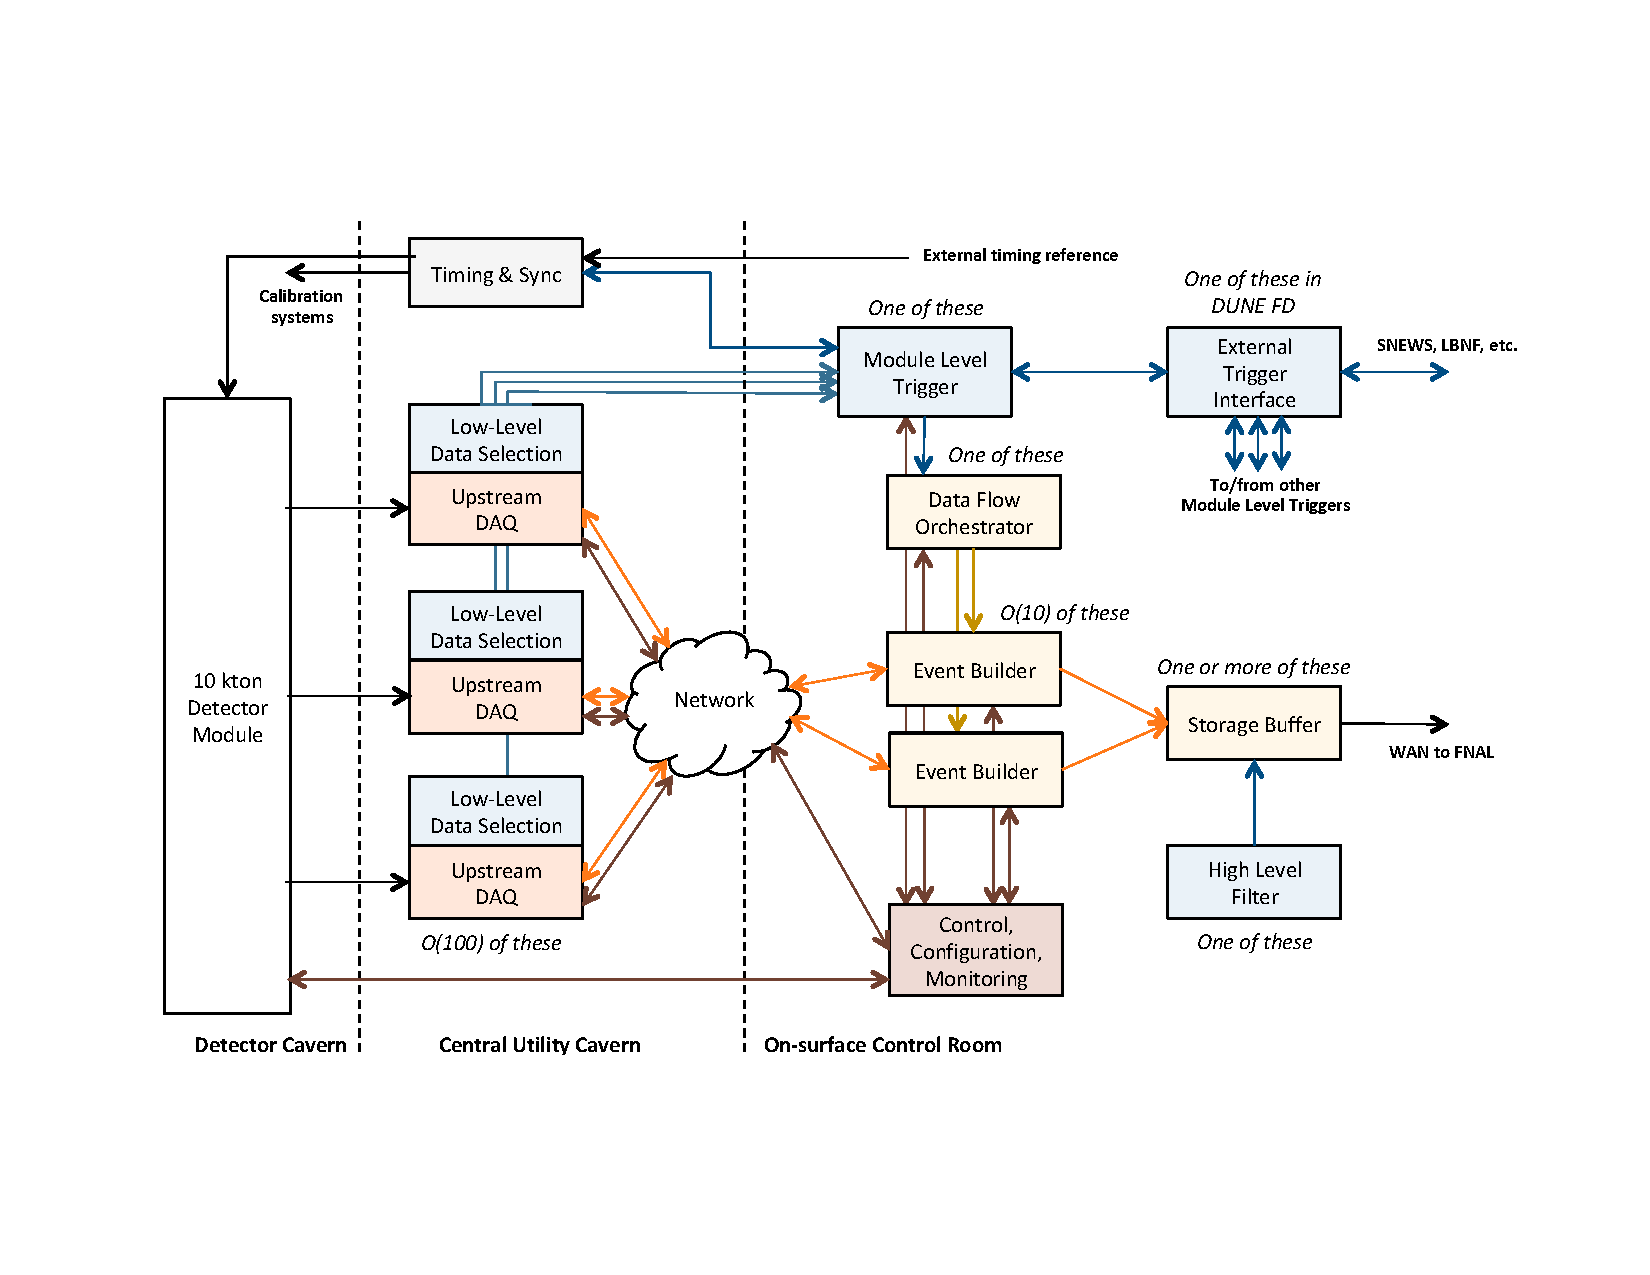
\includegraphics[width=0.8\textwidth,trim=4cm 3cm 4cm 3cm]{daq-layout-2.pdf}
\end{dunefigure}


\subsection{Requirements and Specifications}
\label{sec:daq:requirements}

The \dword{dune} \dword{fd} \dword{daq} system is designed to meet the
\dword{dune} top-level as well as \dword{daq}-level requirements
summarized in Table~\ref{tab:rec-specs:SP-DAQ}. The \dword{daq}-level requirements are
imposed to ensure that the 
system %is capable of 
can record all necessary information for offline 
analysis of data that is associated with on- and off-beam physics events, as directed
by the \dword{dune} physics mission, and with minimal compromise to
\dword{dune}'s physics sensitivity. The requirements must be met by following the 
specifications provided in the same table. Those specifications are
associated with trigger functionality, readout considerations,
and operations considerations, and are motivated further in the following subsections.

\subsubsection{How DUNE's Physics Mission Drives the DAQ Design}

The DUNE Far Detector has three main physics drivers: neutrino \dword{cpv} and related
long baseline oscillation studies using the high intensity beam provided
by \fnal, off-beam measurements of atmospheric neutrinos and searches
for rare processes such baryon-number-violating decays,
and detection of neutrinos from a \dfirst{snb} occurring within our galaxy. The
\dword{dune} \dword{fd} \dword{daq} system must facilitate data
readout for delivering on these main physics drivers, while keeping
within physical (space, power) and resource constraints for
the system. In particular, the off-beam measurements require the
continuous readout of the detector, and the lack of external triggers for such
events requires real-time or online data processing, and
self-triggering capabilities. Since the
continuous raw data rate of the far detector module, as received by
the DAQ system, reaches multiple
terabits per second, significant data buffering and processing
resources are needed as part of the design.

The \dword{dune} \dword{fd} modules employ two active detector components from
which the DAQ system must acquire data: the \dfirst{tpc} and the
\dfirst{pds}. The two components access the physics %each
by sensing and collecting signals associated with very different sensing time
scales.
Ionization charge measurement by the \dword{tpc} for any given activity in the
detector requires a nominal recording of data over a time window of order
\SIrange{1}{10}{\milli\second}. 
This time scale is determined by the ionization electron drift speed in \lar and
the detector dimension along the drift direction. 
On the other hand, the \dword{pds} measures argon scintillation light emission,
which occurs and is detected over a timescale of multiple nanoseconds to
microseconds for any given event and/or subsequent subevent process.
Both the TPC and the PDS data are compressed by the front-end electronics prior
to input to the DAQ.
 
Figure \ref{fig:daq-rates} provides the expected activity rates in a
single far detector module as a function of true energy associated
with given types of signal.
At low energy ($<$10 MeV), activity is dominated by radiological backgrounds
intrinsic to the detector, and
low-energy solar neutrino interactions. Supernova burst neutrinos,
expected to arrive at a galactic \dword{snb} rate of once per century, 
would span the 10-30 MeV range. At higher energies (generally
above 100 MeV), rates are dominated by cosmic rays, beam neutrino interactions,
and atmospheric neutrino interactions. With the exception of supernova
burst neutrinos, the activity associated with any of these physics
signals is localized in space and particularly in time. Supernova burst
neutrinos on the other hand are characteristically different, as they arrive as multiple
signals of localized activity that extends over the entirety of the
detector and over multiple seconds.

The nature and rates of these signatures necessitates a data selection strategy
which handles two distinct cases: a localized high-energy activity trigger,
prompting an event record readout for activity associated with a minimum of 100
MeV of deposited energy; and an extended low-energy activity trigger, prompting
an event record readout when multiple localized low-energy activity candidates
with low deposited energy each are found over a short (less than 10 seconds)
time period and over the entirety of a 10 kton module. 
Because of the high granularity of the detector readout elements, a hierarchical
data selection subsystem is employed to provide data processing and triggering,
and facilitate optional data reduction and filtering.
The DAQ system is required to yield $>$99\% efficiency for particles depositing
$>$100 MeV of energy in the detector, for localized high-energy triggers; it is
also required to yield sufficient efficiency for low-energy deposition in the
detector as needed to yield $>$90\% galactic supernova burst trigger coverage,
for extended low-energy triggers.
Galactic coverage is defined as the supernova burst trigger efficiency, weighted
by the probability of a galactic supernova burst (which is galactic
distance-dependent).

By offline considerations, the DAQ is limited to sending no more than 30 PB per
year to offline.
As such, the steady state rate of localized triggers from the entire far
detector (including all four modules) is effectively limited to less than 0.1
Hz, otherwise more than 30 PB of data (uncompressed) would be generated per
year.
This assumes (conservatively) that each localized high-energy trigger prompts
\dpreadout of losslessly compressed TPC data plus lossy compressed PDS data over
the same duration from the entire module to be read out as part of the event
record.
The average rate of supernova burst triggers (the vast majority of which are
false-positive) is limited to 1 per month, per similar considerations; this
assumes that an extended low-energy trigger prompts 100 s of losslessly
compressed data from the entire module to be read out as part of the event
record.
The average monthly SNB trigger would amount to a 7\% addition to the total data
volume generated by a 0.1 Hz localized trigger rate.

The capability of recording data losslessly is built into the design as a
conservative measure; a particular concern is charge collection efficiency in
the case of zero suppression. 
MicroBooNE is currently investigating the impact of zero suppression on
reconstruction efficiency and energy resolution for low-energy events. 
Expected data rates from physics signals of interest, which fit the 30 PB yearly
generated volume and trigger rate requirements, are summarized in
Table~\ref{tab:daq:rates}.

\begin{dunefigure}{fig:daq-rates}{Expected physics-related activity
    rates in a single \SI{10}{\kilo\tonne} module. \label{sec:daq:rates}
}
  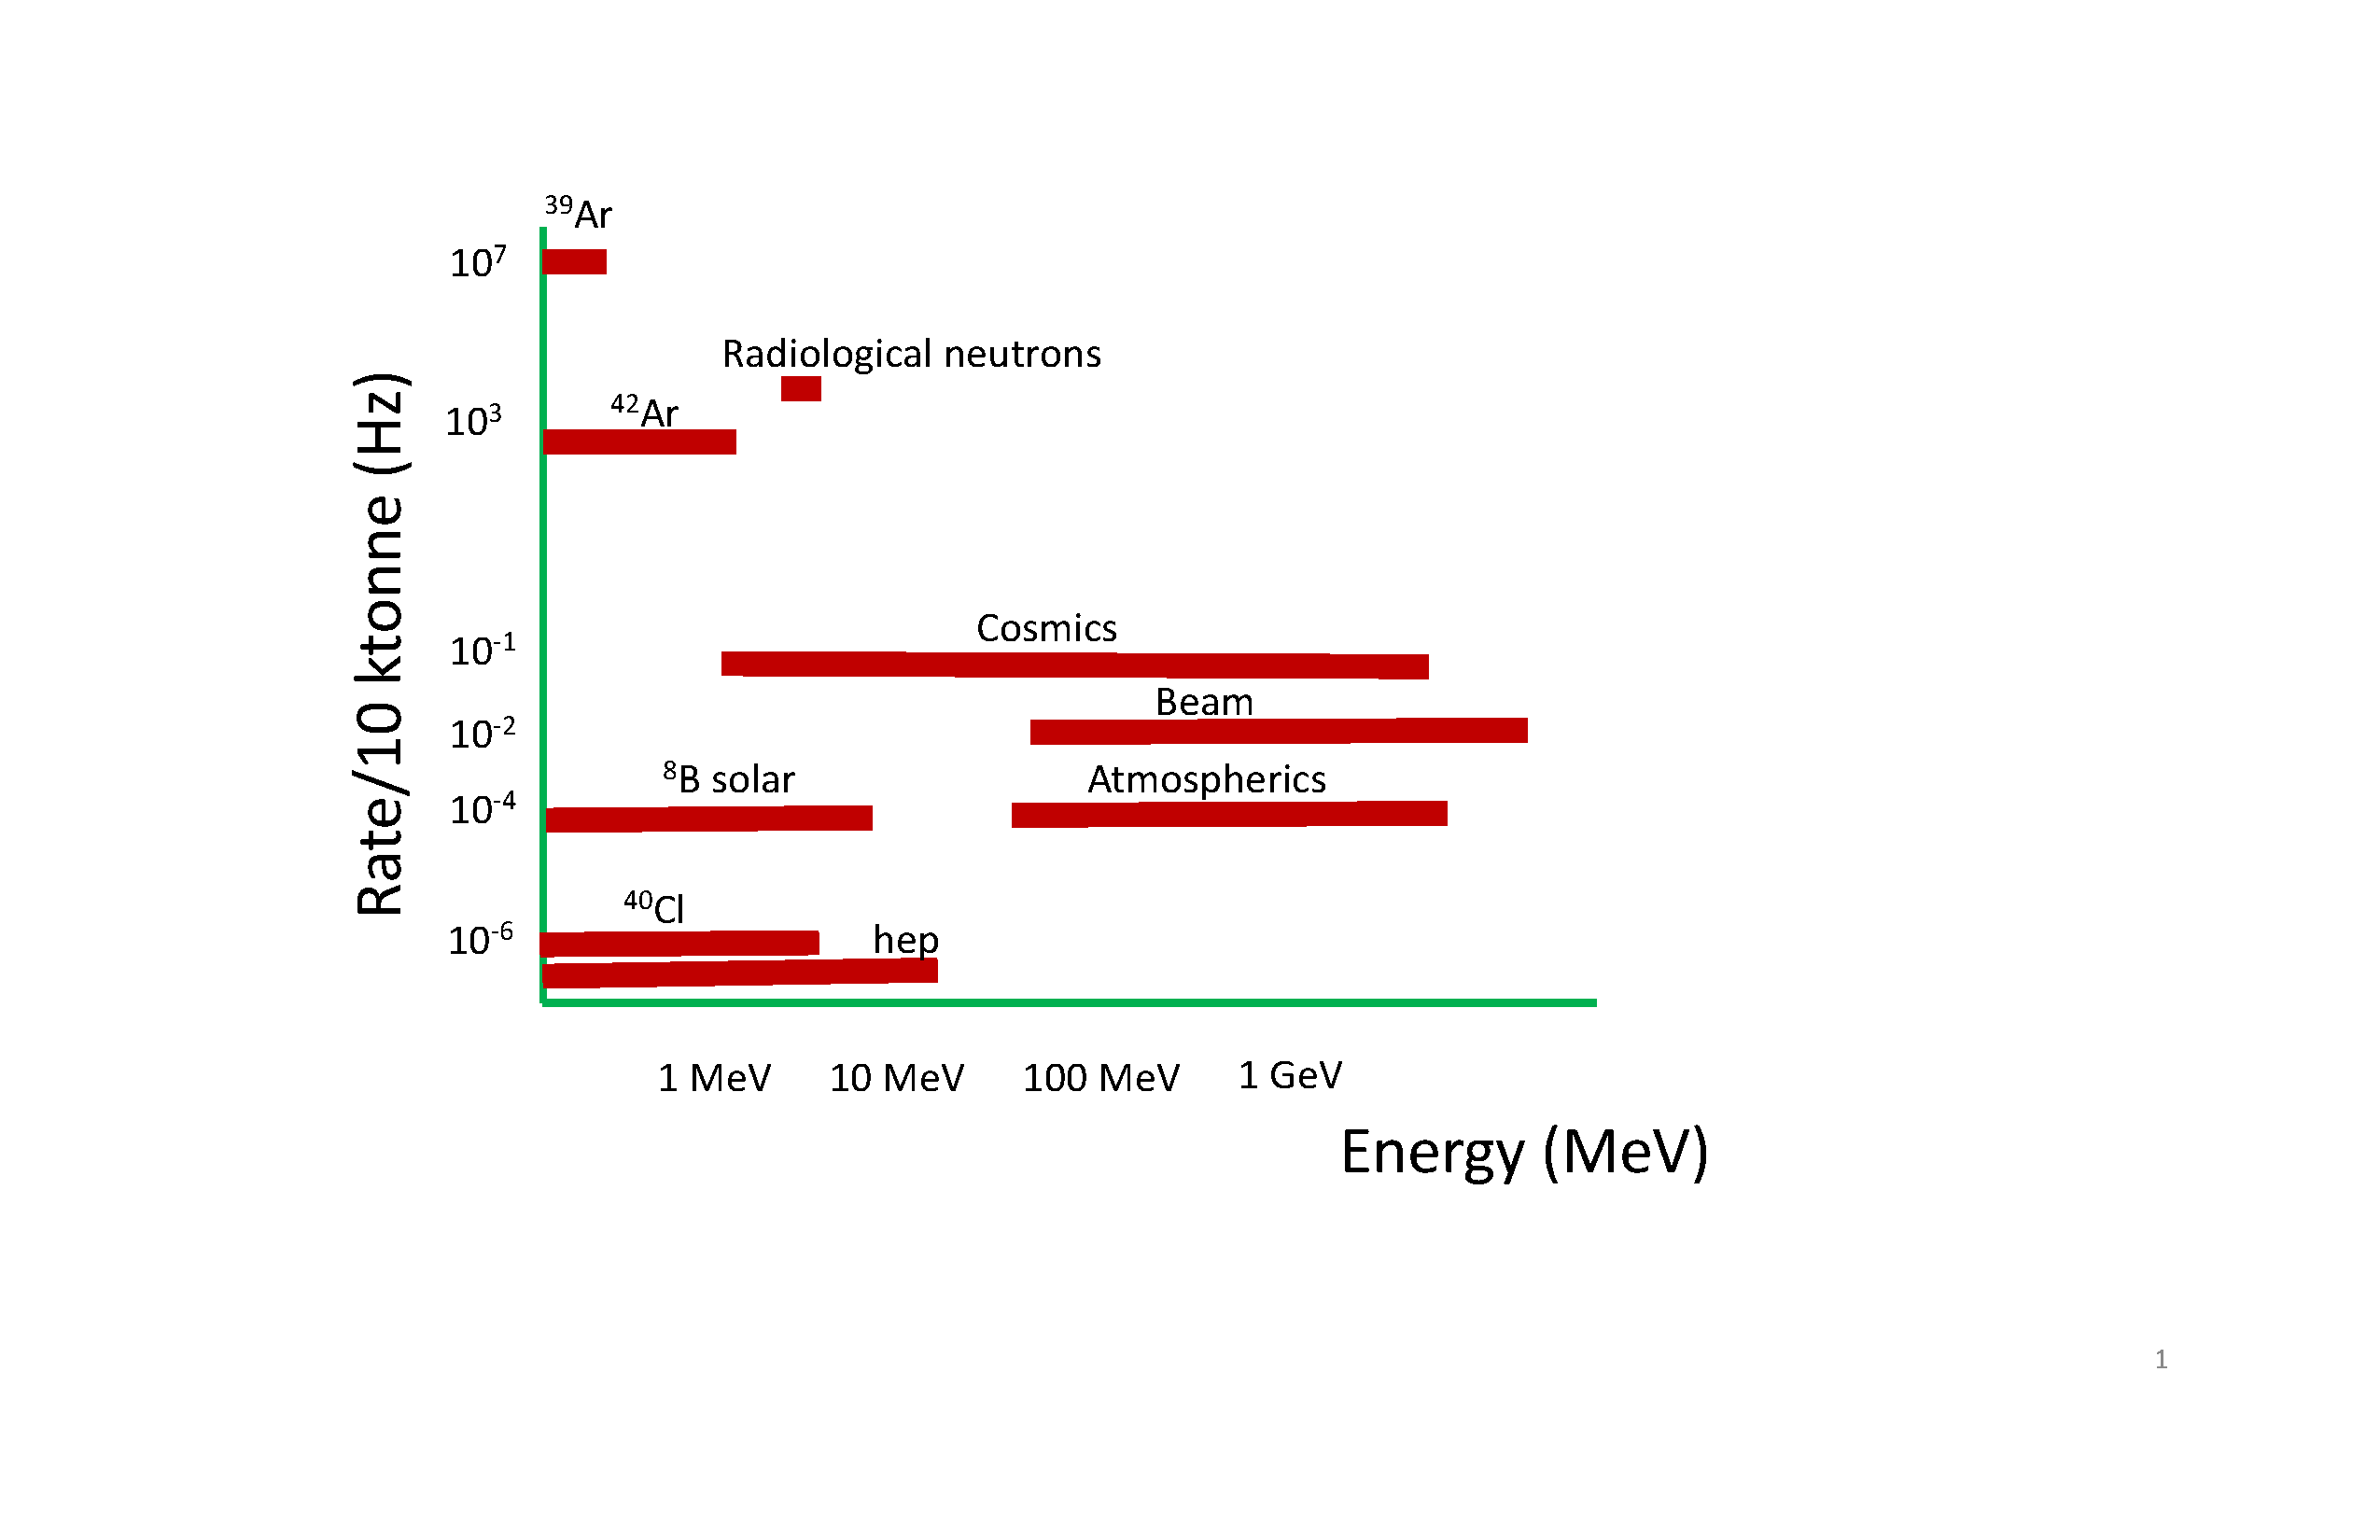
\includegraphics[width=0.7\textwidth,clip,trim=6cm 6cm 10cm 2cm]{daq-event-type-rates-vs-energy.pdf}
\end{dunefigure}

\begin{dunetable}
[Expected DAQ Yearly Data Rates]
{p{0.25\textwidth}p{0.1\textwidth}p{0.5\textwidth}}
{tab:daq:rates}{Summary
    of expected data rates. The rates assume no compression, and are
    given for a single \SI{10}{\kilo\tonne} module. Trigger primitives
    (see Section~\ref{sec:daq:design-data-selection})
  are not kept permanently; they are temporarily stored for 1-2 months
  at a time.  
%  \fixme{These numbers are for SP and must be replaced with DP numbers.}
}
Source  & Annual Data Volume & Assumptions \\\toprowrule
Beam interactions & 7 TB & 10 MeV threshold in coincidence with beam
time, including cosmic coincidence; \SI{7.5}{\milli\second} readout \\\colhline
Cosmics and atmospheric neutrinos & 2.33 PB & \SI{7.5}{\milli\second} readout \\\colhline
Radiological backgrounds & $<0.72$ PB & $<1$ per month fake rate for SNB
trigger\\\colhline
Cold Electronics calibration & 200 TB & \\\colhline
Radioactive source calibration & 100 TB & $<10$ Hz source rate; single
CRP readout; \SI{7.5}{\milli\second} readout \\\colhline
Laser calibration & 200 TB & 10$^6$ total laser pulses; half the
TPC channels illuminated per pulse; lossy
compression (zero-suppression) on all channels\\\colhline
Random triggers & 60 TB & 45 per day\\\colhline
Trigger primitives & $15.3$ PB & Dominated by $^{39}$Ar (150~kHz per CRP); two collection
views; 20 bytes per trigger primitive \\\colhline
\end{dunetable}

Self-triggering on \dword{snb} activity is a unique challenge for the DUNE FD,
and an aspect of the design which has never been demonstrated in a LArTPC.
The challenge with \dword{snb} triggering is two-fold. 
First, the activity of the individual \dword{snb} neutrino interactions is
expected to be of relatively low energy (\SIrange{10}{30}{\mega\electronvolt}),
sometimes indistinguishable from pile-up of radiological background activity in
the detector.
Triggering on an ensemble of \bigo{100} events expected on average in the case
of a galactic supernova burst is therefore advantageous; however, since this
ensemble of events is expected to occur sparsely over the entire detector and
over an extended period of \bigo{10}\si{s}, sufficient buffering capability must
be designed into the system to capture the corresponding signals. 
Furthermore, to ensure high efficiency in collecting \dword{snb} interactions
that, individually, are below low-energy activity threshold, data from all
channels in the detector will be recorded over an extended and contiguous period
of time \bigo{100}\si{s} around every \dword{snb} trigger.

% % This file is generated, any edits may be lost.
\begin{footnotesize}
%\begin{longtable}{p{0.14\textwidth}p{0.13\textwidth}p{0.18\textwidth}p{0.22\textwidth}p{0.20\textwidth}}
\begin{longtable}{p{0.12\textwidth}p{0.18\textwidth}p{0.17\textwidth}p{0.25\textwidth}p{0.16\textwidth}}
\caption{Specifications for DP-DAQ \fixmehl{ref \texttt{tab:spec:DP-DAQ}}} \\
  \rowcolor{dunesky}
       Label & Description  & Specification \newline (Goal) & Rationale & Validation \\  \colhline


   
  \newtag{DP-DAQ-1}{ spec:DAQ-readout }  & DAQ readout throughput: The DAQ shall be able to accept the continuous, compressed data stream from the TPC and Photon detectors.  &  \SI{65}{GB/s} per dual phase detector module &  Specification from TPC and PDS electronics &  Modular test on test bench; overall throughput scales linearly with the number of electronics crates.  \\ \colhline
    
   
  \newtag{DP-DAQ-2}{ spec:DAQ-throughput }  & DAQ storage throughput: The DAQ shall be able to store selected data at an average throughput of 2 Gb/s, with temporary peak throughput of 100 Gb/s.  &  \SI{2}{GB/s} average storage throughput; \SI{100}{GB/s} peak temporary storage throughput per dual phase detector module &  Average throughput estimated from physics and calibration requirements; peak throughput allowing for fast storage of SNB data.  &  ProtoDUNE demonstrated steady storage at $\sim$ 40 Gb/s for a storage volume of 700 TB. Laboratory tests will allow to demonstrate the performance reach. \\ \colhline
    


\label{tab:specs:DP-DAQ}
\end{longtable}
\end{footnotesize} 
\fixme{Need DP-DAQ reqs/specs spreadsheed and generated table.}


\subsubsection{Practical Considerations for Design}

The DAQ system is designed as a single, scalable system which can service all FD
modules.
It is also designed on the principle that the system should be able to record
and store full detector data with zero dead time; and that it should be
evolutionary, taking advantage of the staged construction for the DUNE FD, and
thus beginning very conservatively for the first DUNE FD module, and agressively
reducing the design conservatism as further experience is gained with detector
operations.
At the same time, it is designed to preserve the possibility of additional
capacity as required.
The bulk of processing and buffering of raw detector data is done underground,
in the upstream DAQ part of the system (see Figure~\ref{fig:daq:layout}), in
order to minimize data traffic to surface.
Power, cooling, and space constraints in the CUC are limited to 600 kW total and
52 racks for all four FD modules.

There are three key challenges for the DUNE FD DAQ system: 
\begin{itemize}
\item First, the system must accommodate a long (``permanent'') commissioning
  state for the far detector, and must therefore be a fully ``partitionable''
  system. 

  Given operational considerations, and in particular based on the need to
  minimize \dword{snb} dead time, partitioning the \dword{daq} system allows a
  significant portion of the detector to remain physics-operational even if a
  fault interrupts data collection in some part of the detector. 
  This partitionable operation mode also permits detector development and
  specialized runs (e.g.,~calibrations) to run in parallel with normal physics
  data taking, for small subsets of the detector.

\item Secondly, the \dword{snb} physics requirements necessitate large buffering
  in the upstream DAQ and low fake supernova burst trigger rates. 

  The implementation of a continuous storage element in the data flow
  architecture allows for the formation and capture of delayed, data-driven
  trigger decisions with minimal loss of physics information.
  The specification for this look-back buffer is set in consultation with
  physics groups.
  The buffer size is driven primarily by the need to record up to ten seconds of
  unbiased data preceding a \dword{snb} (with the neutronization time taken as
  the time of the burst), and it is specified to be greater than four seconds.
  This four-second buffering provision works in tandem with a trigger latency
  specification of less than one second.
  This aspect remains to be validated with simulation, to ensure that high
  coverage (greater than 90\%) for galactic \dwords{snb} is achieved by the
  \dword{snb} trigger.

  The \dword{daq} system is also designed so as to be able to apply lossless
  compression to these records, as well as filter them to remove unnecessary
  data regions in an intelligent way, i.e.~without compromising physics
  performance.

  A programmable trigger priority scheme ensures that the readout for the main
  physics triggers is never or rarely inhibited so as to enable easy
  determination of the live-time of these triggers. 
  At the same time, generation of overlapping triggers will be possible, and
  ordering and prioritization will prevent data readout duplication. 

\item Finally, the difficult-to-access underground location requires that the
  DAQ operates with high reliability and fully remote operation.

  Furthermore, to ensure minimal impact to overall detector live-time, the
  \dword{daq} system is fully configurable, controllable, and operable from
  remote locations, with authentication implemented to allow exclusive control.
  The DAQ furthermore facilitates online monitoring of the detector and of
  itself.

\end{itemize}

\subsection{Summary of Key Parameters}
\label{sec:daq:parameters}

Table~\ref{tab:daq:parameters} summarizes the important parameters driving the
\dword{daq} design. 
These parameters set the scale of data buffering,
processing, and transferring resources which must be built into the design of
each \dword{fd} module. 

\begin{dunetable}
[Key \dword{daq} Parameters]
{ll}
{tab:daq:parameters}
{Summary of important parameters driving the \dword{daq} design.  
%\fixme{These   are SP numbers and must be replaced with DP equivalents.  Note, many of
%    these numbers are already in or should be added to \texttt{common/defs.tex}}
}
Parameter & Value \\ \toprowrule
TPC Channel Count per Module & 153,600\\ \colhline
TPC Collection Channel Count per Subdetector (CRP) & 1920\\ \colhline
PDS Channel Count per Module & 720\\ \colhline
TPC \dword{adc} Sampling Rate & 2,5 MHz\\ \colhline
TPC \dword{adc} Dynamic Range& 12 bits\\ \colhline
PDS \dword{adc} Sampling Rate & TBD \\ \colhline
PDS \dword{adc} Dynamic Range & TBD \\ \colhline
PDS \dword{adc} Readout Length & TBD \\ \colhline
Localized Event Record Window & \SI{7.5}{\milli\second}\\  \colhline
Extended Event Record Window &  100 s\\  \colhline
Full size of TPC Localized Event Record per Module (uncompressed) & 4.2 GB \\  \colhline
Full size of TPC Extended Event Record per Module (uncompressed) & 56 TB\\  \colhline
Full size of PDS Localized Event Record per Module & TBD \\  \colhline
Full size of PDS Extended Event Record per Module & TBD \\  \colhline
\end{dunetable}


\subsection{Interfaces}
\label{sec:daq:interfaces}

The \dword{daq} system scope begins at the optical fibers streaming compressed
digital data from the electronics servicing the active detector components (TPC
and PDS), and ends at a wide area network (WAN) interface that distributes the
data from on site at \surf to offline centers off site.
The \dword{daq} also provides common computing and network services for other
\dword{dune} systems, although slow control and safety functions fall outside
\dword{daq} scope.

Consequently, the \dword{dune} \dword{fd} \dword{daq} system interfaces with the dual-phase TPC electronics, computing, \dword{cisc}, and calibration systems of the %\dword{dune}
\dword{fd}, as well as with facilities and underground installation. The
 interface agreements with the \dword{fd} systems 
are listed in Table~\ref{tab:daq:interfaces}, and described
briefly in the following subsections. Interface agreements with
facilities and underground installation are described in Section~\ref{sec:daq:production}.

\fixme{Add summaries in table. Georgia}
\begin{dunetable}
[\dword{daq} System Interface Links]
{p{0.3\textwidth}p{0.3\textwidth}p{0.2\textwidth}}
{tab:daq:interfaces}
{Data Acquisition System Interface Links.

% \fixme{Some of these are SP interface   documents and need to be replaced with DP versions.}
}
Interfacing System & Description & Reference \\ \toprowrule
DP Electronics  & & \citedocdb{6778}\\ \colhline
PDS Readout & &  \citedocdb{6727}{v2} \\ \colhline
Computing &&  \citedocdb{7123} \\ \colhline
CISC & & \citedocdb{6790}{v1} \\ \colhline
Calibration & Constraint on total volume of the calibration data;
trigger and timing distribution from the DAQ & \citedocdb{7069} \\ \colhline
Timing and Synchronization &&  \citedocdb{11224} \\ \colhline
Integration Facility & & \citedocdb{7042}{v0} \\
Facilities &&  \citedocdb{6988}{v1} \\ \colhline
\end{dunetable}

\begin{description}
\item[TPC Electronics] The \dword{daq} and TPC Electronics interface is
  described in \citedocdb{6778}.
  The physical interface is in the \dword{cuc}, where optical links from the
  \dword{cro} and \dword{lro} microTCA crates which transfer their compressed data to the
  \dword{daq} \dword{fe} readout (\dword{felix}; see
  Section~\ref{sec:daq:design-upstream}).
  This ensures the \dword{daq} is electically decoupled from the detector
  cryostat.
  One \SI{10}{Gbps} link per each electronics readout is expected, and has been
  specified as 300m OM4 multi-mode fibers from sfp+ at the
    crate 
%{This is what WIBs use, what about DP crates?}
  to \dword{minipod} on \dword{felix}.

The data format employs for the charge readout lossless compression, achieved with an optimized version of the Huffman algorithm.  Compression on average reduces by a factor 10 the data volume.  The typical occupancy of a 10 Gbit/s data link is then around 2 Gbit/s. The communication protocol is UDP. Data are organized in jumbo frames with MTU 9000 bytes. Each charge readout crate includes ten AMC cards, each digitizing 64 channels. The data on the AMC are compressed on the fly, stored on a local memory buffer and continuously streamed to the DAQ.  Data are transmitted by the AMCs to the DAQ, organized in contiguous time-windows. Time-windows are exactly synchronized on the entire detector front-end, thanks to the fact  that the sampling on all AMC is absolutely aligned with respect to the UTC via the White-Rabbit system.  At the beginning of each time window the data compression sequence is reinitialized on all AMC channels starting from the absolute ADC values and the UTC time-stamp of the first sample of the frame is trasmitted in a window-header packet to the DAQ. Then each AMC performs, sequencially for its 64 channels, the transmission of the data packets corresponding to the continuous streaming of the  time-window. Given compression, the number of bytes used to transmit the time-window may change dynamically from channel to channel. An example of possible data format is described in the following, assuming a time-window lasting 3 ms and containing 4k samples per channel. The definition of the time-window lenght is flexible and may be further optimized.  In the given time window the AMC trasmits sequencially its data from channel 1 to channel 64 by exploiting multiple data frames. In order to achieve maximum packing per frame, data from several channels are transmitted in the same frame.  Each data frame starts with a header containing the AMC identifier, the frame number, the number of channels included in the frame, including the last transmitted channel  which may be truncated and have its data sequence overflowing in the next frame. Then the frame header provides the list of channel numbers included in the frame and the corresponding number of bytes to be read for each one of them.  For instance in case of a frame containing compressed data from 3 contiguous channels  (n,n+1,n+2) starting from channel number n : n,n+1,n+2,N1,N2,N3.  Where n+2 is the last channel of the frame which may have its data overflowing in the next frame. Immediately after the header the rest of the frame contains the raw compressed data:  N1 bytes for channel n,  N2 bytes for channel n+1, N3 bytes for channel n+2.  The number of channels treated in a frame may vary depending on the compression efficiency. The data format aims at the maximal  occupancy of the data frames, independently of the instantaneous compression fluctuations.


\item[Computing] The \dword{daq} and computing interface is described in
  \citedocdb{7123}.
  \metainfo{Buffer disk. 
    Agreement on system administration support and computer procurement, ssh
    gateways, non data networks. 
    Address reference how the data model described above is acceptable.}
  The computing consortium is responsible for the online areas of WAN connection
  between \surf and \fnal, while the \dword{daq} consortium is responsible for
  disk buffering to handle any temporary WAN disconnects and the infrastructure
  needed for real-time data quality monitoring. 
  The computing consortium is also responsible for the offline development and
  operation of the tools for data transfers to \fnal.
  The primary constraint in defining the \dword{daq} and offline computing
  interface is the requirement to produce less than \SI{30}{PB/year} for
  transfer to \fnal.
  \dword{daq} and computing consortia are jointly responsible for data format
  definition and data access libraries, as well as real-time data quality
  monitoring software.
  The former is specified in the form of a data model documented in
  \citedocdb{??}.

\item[CISC] The \dword{daq} and \dword{cisc} interface is described in
  \citedocdb{6790}. 
  The \dword{daq} provides a network in the \dword{cuc} for \dword{cisc},
  operation information and hardware monitoring information to \dword{cisc}, and
  power distribution and rack status units in \dword{daq} racks. 
  The information from \dword{cisc} feeds back into the \dword{daq} for run
  control operations.

\item[Calibration] The \dword{daq} and calibration interface is described in
  \citedocdb{7069}.
 Two calibration systems are envisioned 
%{Are these consistent with DP?}
  for the \dword{fd}: a laser calibration
  system and a neutron generator.
  Calibration pulses will be issued by the calibration systems themselves, upon
  receipt of time stamps from the DAQ system; %, and those
  the latter will be issued by the data selection system and distributed through
  the \dword{daq} timing system.

\item[Timing and Synchronization] The timing system of the \dword{dune}
  \dword{fd} connects with almost all detector systems and with the calibration
  system and has a uniform interface to each of them. 
  A single interface document, \citedocdb{11224}, describes all these timing
  interfaces. 
  In particular, the DAQ timing system will interface with the White Rabbit
  implementation of IEEE1588-2008 utilized by the \dword{dpmod} electronics by providing the analog signals
1PPS and  10MHz clock derived from the GPS disciplined oscillator.

  Accuracy of timestamps delivered to detector endpoints will be
  $\pm$\SI{500}{\nano\second} with respect to UTC.
  Synchronization between any two endpoints in the detector will be better than
  \SI{10}{\nano\second} on average.
  Between detector modules, synchronization will be better than
  \SI{25}{\nano\second} on average.
  The timing system will also provide a synchronized clock source by which DAQ
  computer system clocks may be synchronized using standard network time
  protocols.
  System clocks are expected to be synchronized to within a ms using NTP and
  \si{\micro\second} using PTP standards.

\end{description}

\section{Data Acquisition System Design}
\label{sec:daq:design}

This section begins with an overview of the \dword{daq} design followed by
descriptions of the subsystem designs and implementation specifics.
The implementation details are evolving rapidly; as such, more information is
provided in technical notes as listed in Table~\ref{tab:daq:tech-notes}. 

\begin{dunetable}{p{0.7\textwidth}p{0.2\textwidth}}{tab:daq:tech-notes}{Summary of detailed \dword{daq} technical notes on DUNE DAQ subsystem design.}
  Title & Reference \\ \toprowrule
  \dword{dune} \dword{fd} Data Volumes & \citedocdb{9240}\\ \colhline
  The \dword{daq} for the \dword{dune} prototype at CERN &
  \citedocdb{8708}\\ \colhline
 A System for Communication Between \dword{daq} Elements & \citedocdb{10482}\\\colhline
  Data Selection for \dword{dune} Beam and Atmospheric Events & \citedocdb{11215}\\\colhline
  Data orchestrator and event building for \dword{dune} \dword{fd}
  \dword{daq} & t.b.d. \\\colhline
ML-based Data Selecion for DUNE Far Detector & \citedocdb{11311} \\\colhline
 High Level ProtoDUNE tests & \citedocdb{14062} \\ \colhline
  \dword{dune} Run Control, Configuration \& Monitoring (CCM) & t.b.d. \\\colhline
  \dword{dune} \dword{daq} Readout & t.b.d. \\\colhline
  DUNE FD Timing and Synchronization System & \citedocdb{11233} \\\colhline
  What are the DUNE FD \dword{daq} Bottlenecks? & \citedocdb{11461}
  \\\colhline
\end{dunetable}


\subsection{Overview}
\label{sec:daq:design-overview}

The DAQ system is composed of six distinct subsystems: (1) Upstream DAQ
(Section~\ref{sec:daq:design-upstream}), (2) Data Selection
(Section~\ref{sec:daq:design-data-selection}), (3) Back-end DAQ
(Section~\ref{sec:daq:design-backend}), (4) Control, Configration, and
Monitoring (CCM) (Section~\ref{sec:daq:design-run-control}), (5) Timing and
Synchronization (Section~\ref{sec:daq:design-timing}), and (6) Infrastructure
Software.
The physical extent the first five of the DAQ subsystems can be specified in
reference to Figure~\ref{fig:daq:layout}: the Upstream DAQ and Timing and
Synchronization live underground in the CUC; Data Selection occupies both
underground and above-ground spaces; Back-end DAQ is above-ground and includes
data flow orchestration, event building and buffering, before distribution of
data to offline; and CCM extends throughout the entire physical layout of the
system, supported on a private network throughout the DAQ system.
Each of these subsystems is described in further detail in the following
subsections.
To first order, the DAQ system is implemented as an online data processing and
data flow system.
As such, Inter-process Communication (IPC) is an additional, central component
to the FD DAQ, which spans across multiple subsystems, as do other
Infrastructure Software components, e.g.~databases.
Due to its central role, IPC is described below in a separate subsection
(Section~\ref{sec:daq:design-ipc}).

\begin{dunefigure}{fig:daq-conceptual-overview}{\dword{daq} Conceptual
   Overview of DAQ System Functionality for a single 10 kton module}
  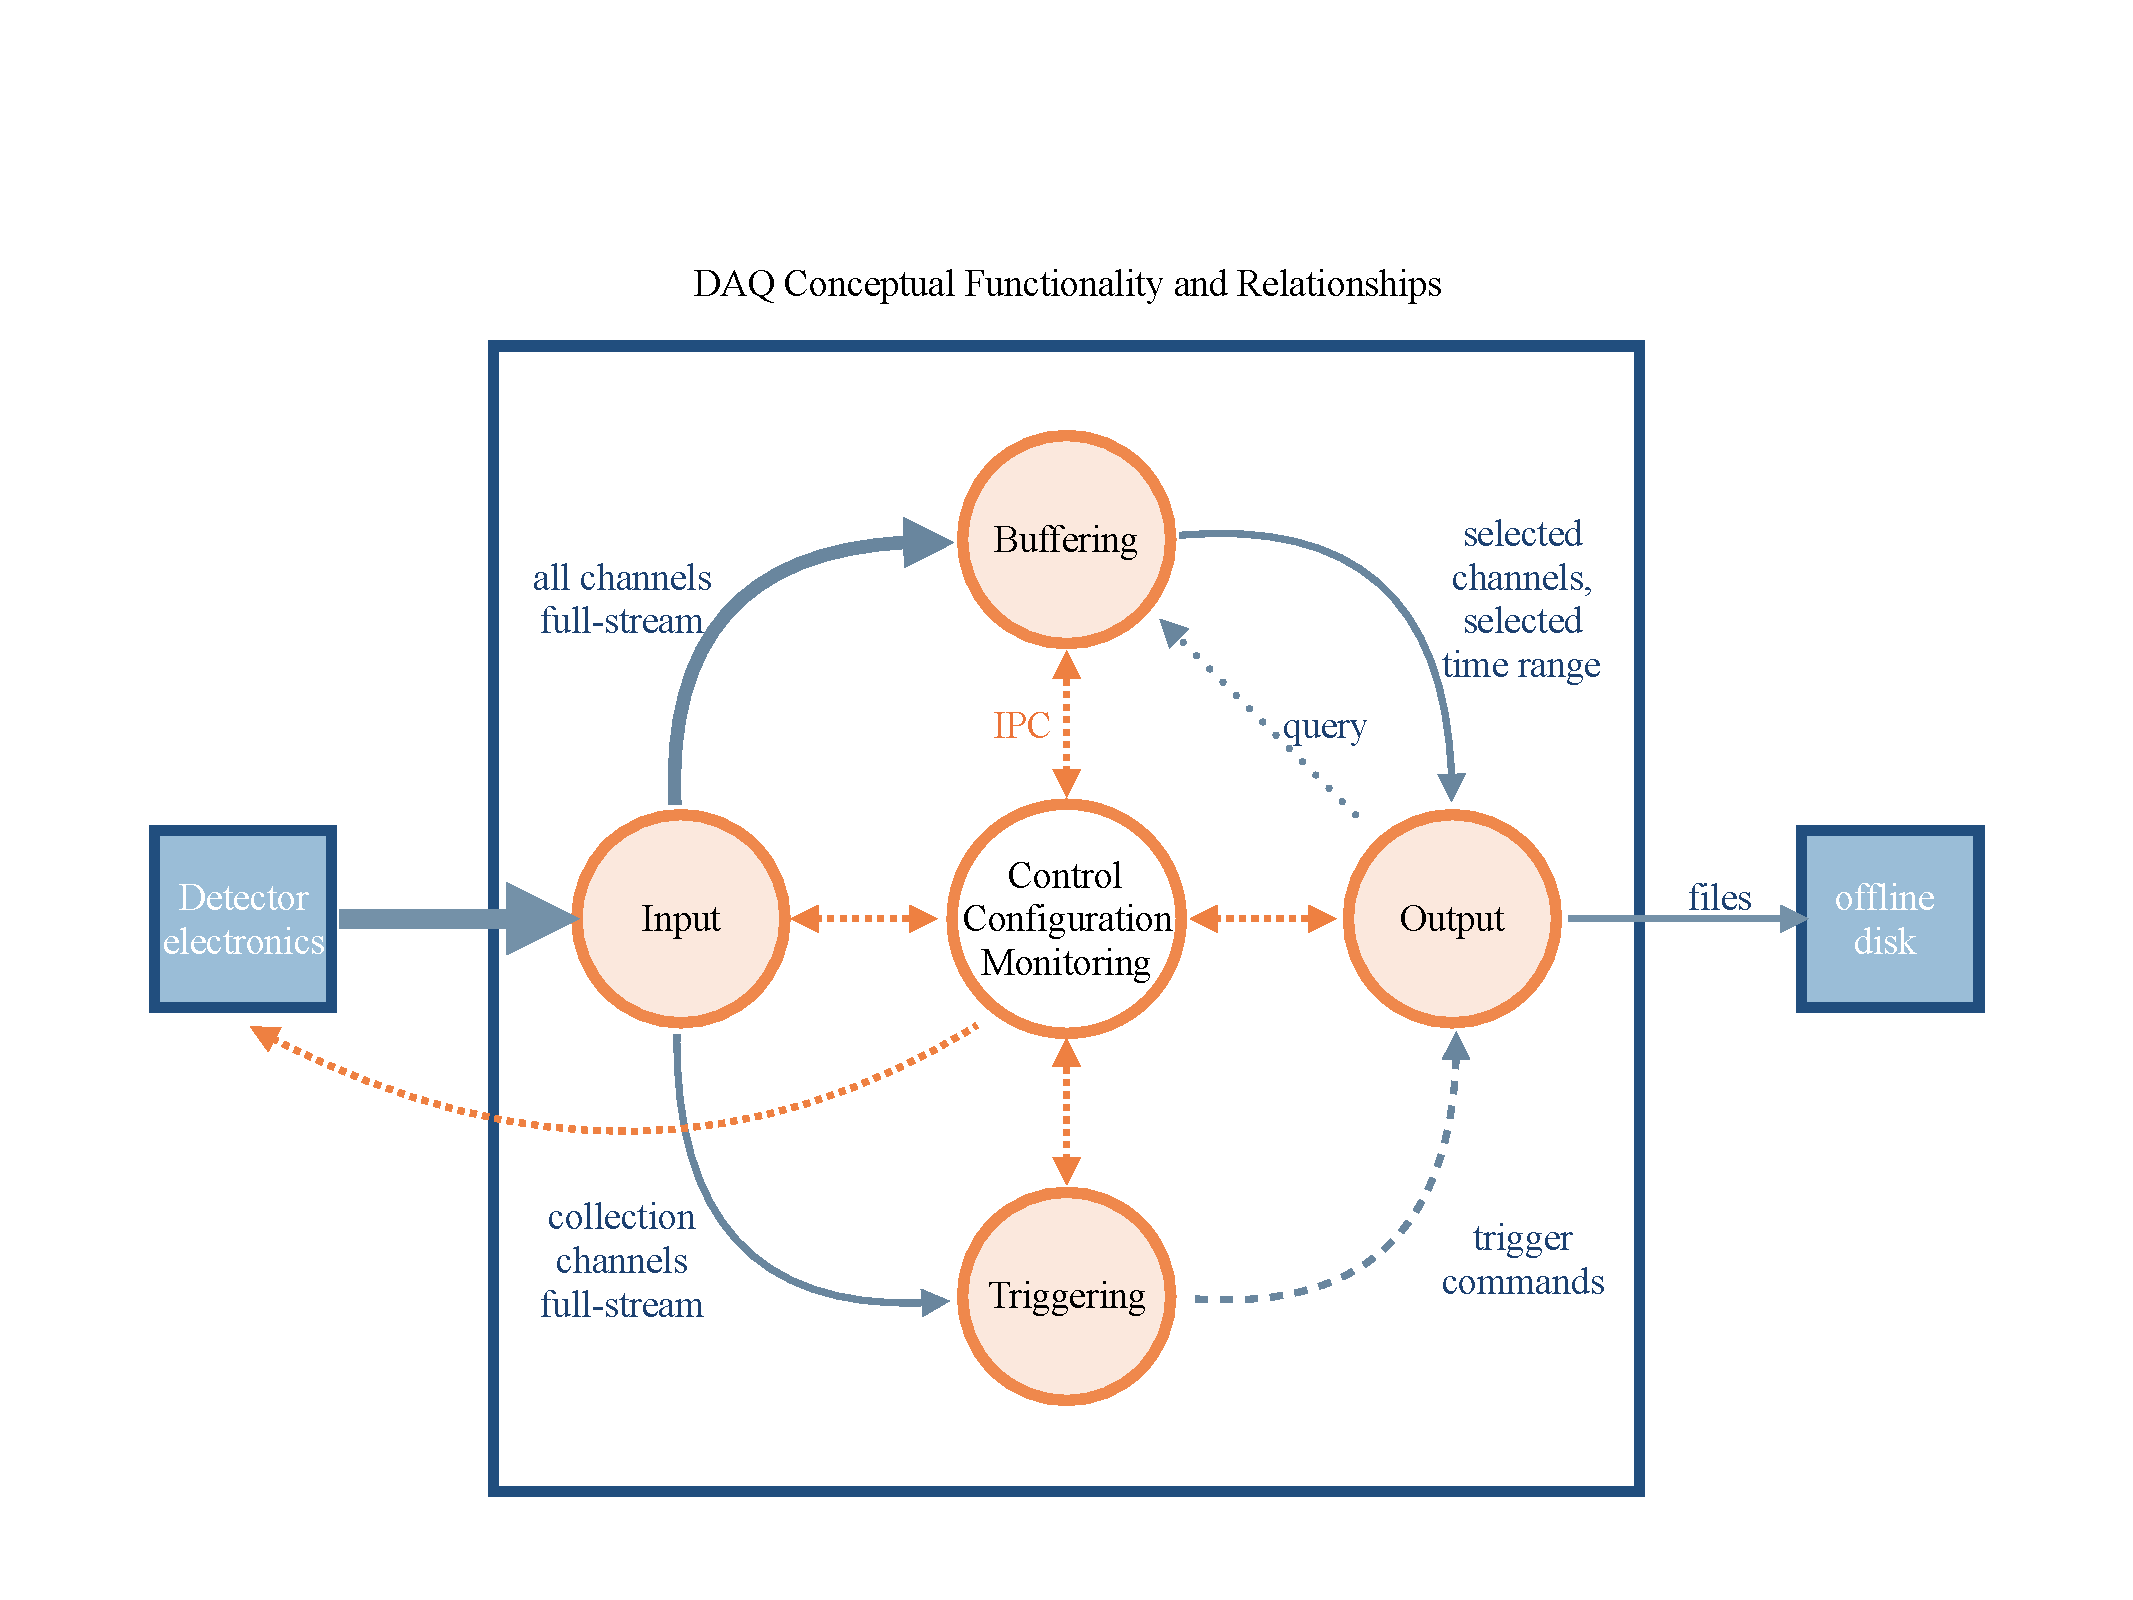
\includegraphics[width=0.8\textwidth]{daq-toplevel-conceptual-nebot.pdf}
\end{dunefigure}


Front-end readout is carried out by the Upstream DAQ, using custom data receiver
and co-processing FPGA/CPU hardware, all of which is hosted in O(100) servers in
the CUC.
A similar number of additional servers is responsible for the execution of
subsequent software-based low-level processing of ``trigger primitives''
generated in the upstream DAQ for the purposes of data selection; the collective
low-level information (trigger primitives and ``trigger candidates'' constructed
from trigger primitives) is propagated to a central server responsible for
further processing and module-level triggering; the module level trigger also
interfaces to a second server which is responsible for receiving and propagating
cross-module and external trigger and timing information.
The module level trigger considers trigger candidates and external trigger
inputs in issuing a ``trigger command'' to the back-end DAQ subsystem.
The Back-end DAQ subsystem facilitates event building in O(10) servers and
buffering for built events on non-volatile storage; upon receiving a trigger
command, the back-end DAQ queries data from the upstream DAQ buffers and builds
that into an ``event record'', which is temporarily stored as (a number of)
files.
Event records can be optionally processed in a high-level filter/data reduction
stage, which is part of overall data selection, prior to event records being
shipped to DUNE offline.
Pervasively, the \dfirst{daqccm} subsystem provides the central orchestration
(Section~\ref{sec:daq:design-run-control}), \dfirst{ipc} provides overall
communication (Section~\ref{sec:daq:design-ipc}), and the \dfirst{daqtss}
provides synchronization (Section~\ref{sec:daq:design-timing}).
Figure~\ref{fig:daq-conceptual-overview} provides a conceptual illustration of
the overal DAQ system functionality, while Figure~\ref{fig:daq-design} specifies
the design implementation. 

\begin{dunefigure}{fig:daq-design}{\dword{daq} DAQ Design Implementation for a
    single 10 kton module}
  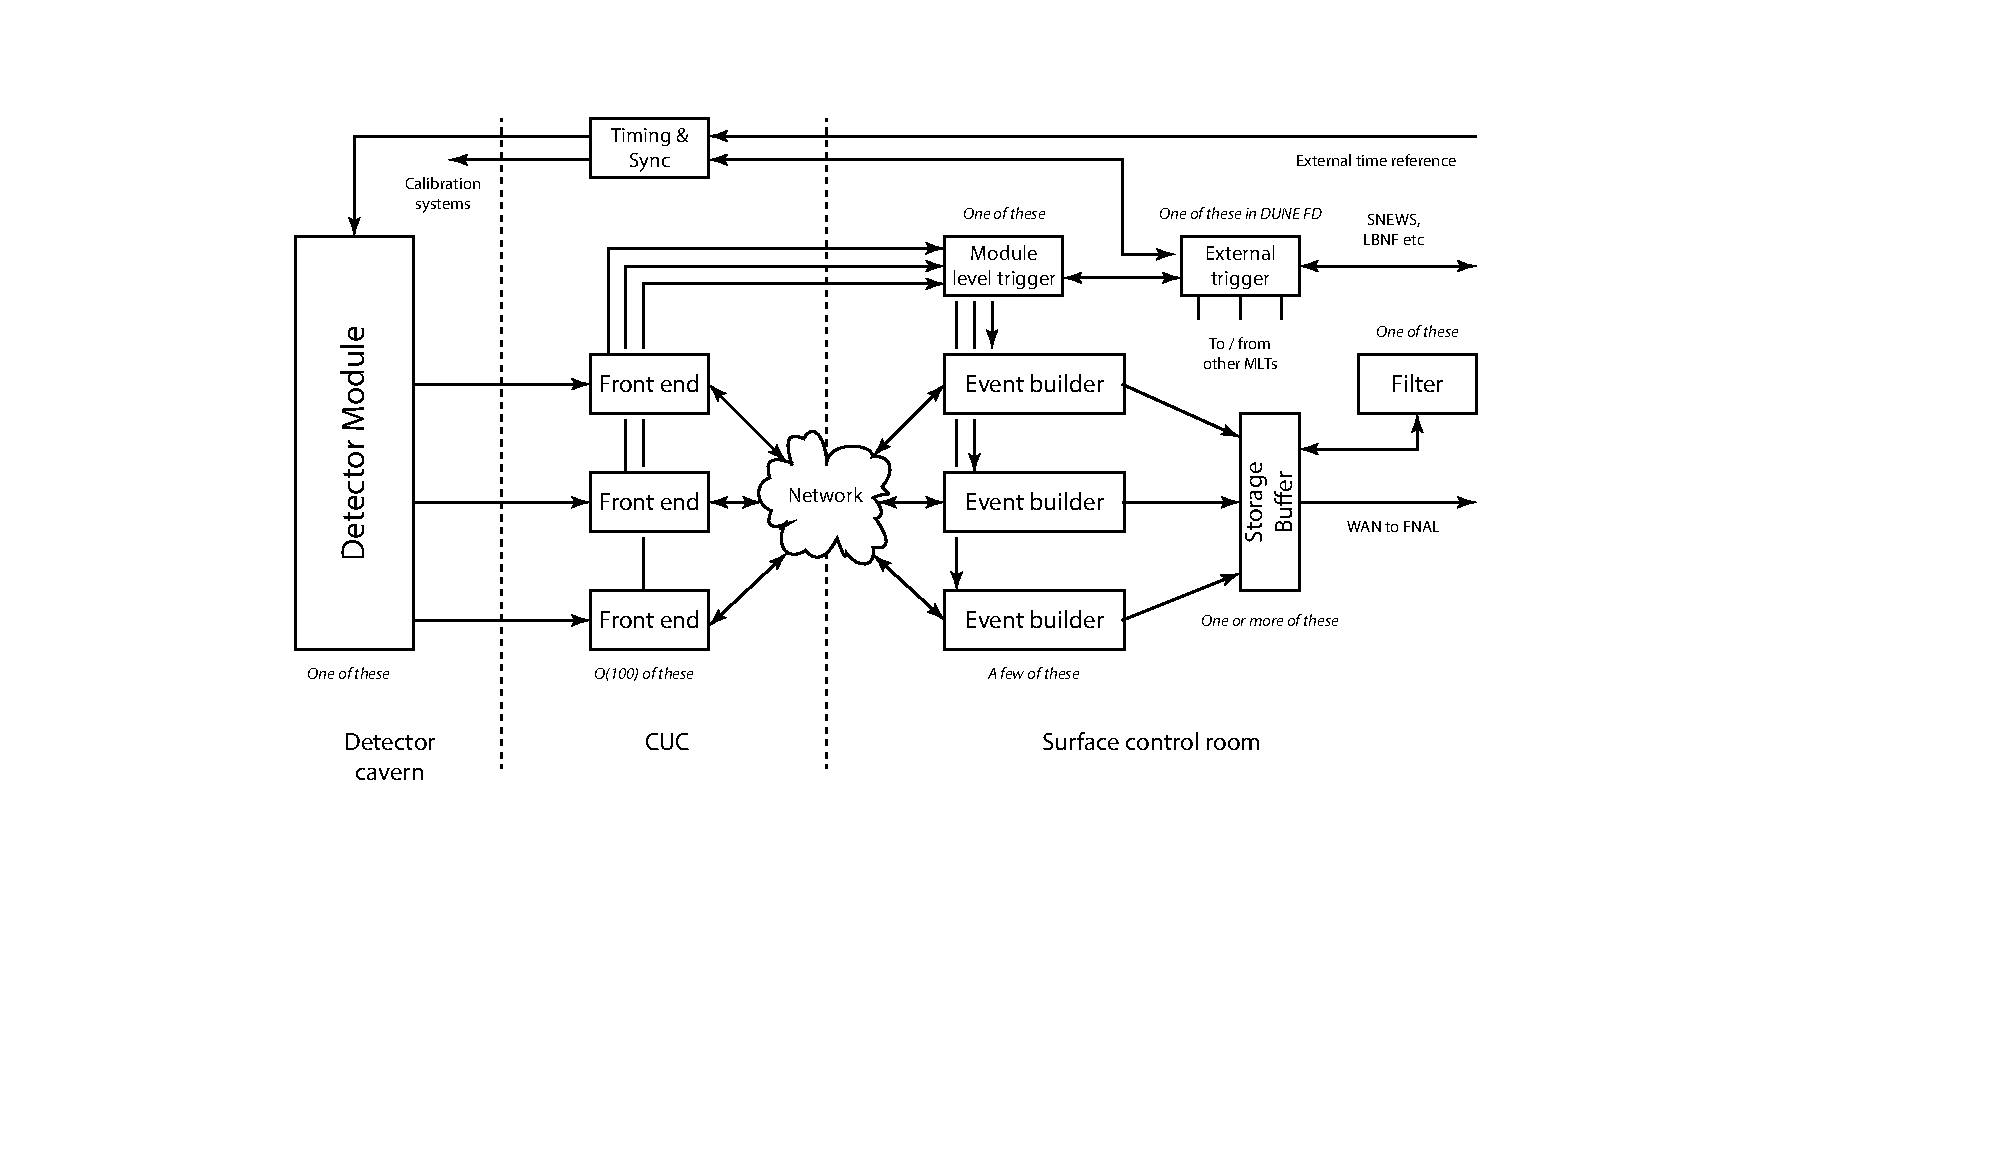
\includegraphics[width=0.8\textwidth]{daq-overview.pdf}
\end{dunefigure}

Key to the implementation of the DAQ design is the requirement that the system
is partitionable.
Specifically, the system can operate in the form of multiple independent DAQ
instances, each executed across all DAQ subsystems and uniquely mapped among
subsystem components. 
More specifically, a given partition may span the entire \dword{detmodule} or
some subset of it; its extent is configurable at run start.
This ensures continual readout of the majority of the detector in normal physics
data-taking run mode, while enabling simultaneous calibration or test runs of
small portion(s) of the detector without interruption of normal data-taking. 

\subsection{Upstream DAQ}
\label{sec:daq:design-upstream}

The Upstream DAQ provides the first link in the data flow chain of the
\dword{daq} system and is where raw data from detector electronics is received
by the DAQ.
It implements a receiver, buffer, and a portion of low-level data selection
(trigger primitive generation; see Section~\ref{sec:daq:design-data-selection})
as detailed in Figure~\ref{fig:daq:readout}.
It is physically connected to the detector electronics via optical fiber(s) and
buffers and serves data to other \dword{daq} subsystems, namely the
\dword{daqdsn} and the back-end DAQ.

\begin{dunefigure}{fig:daq:readout}{\dword{dune} upstream \dword{daq} subsystem and its connections.}
  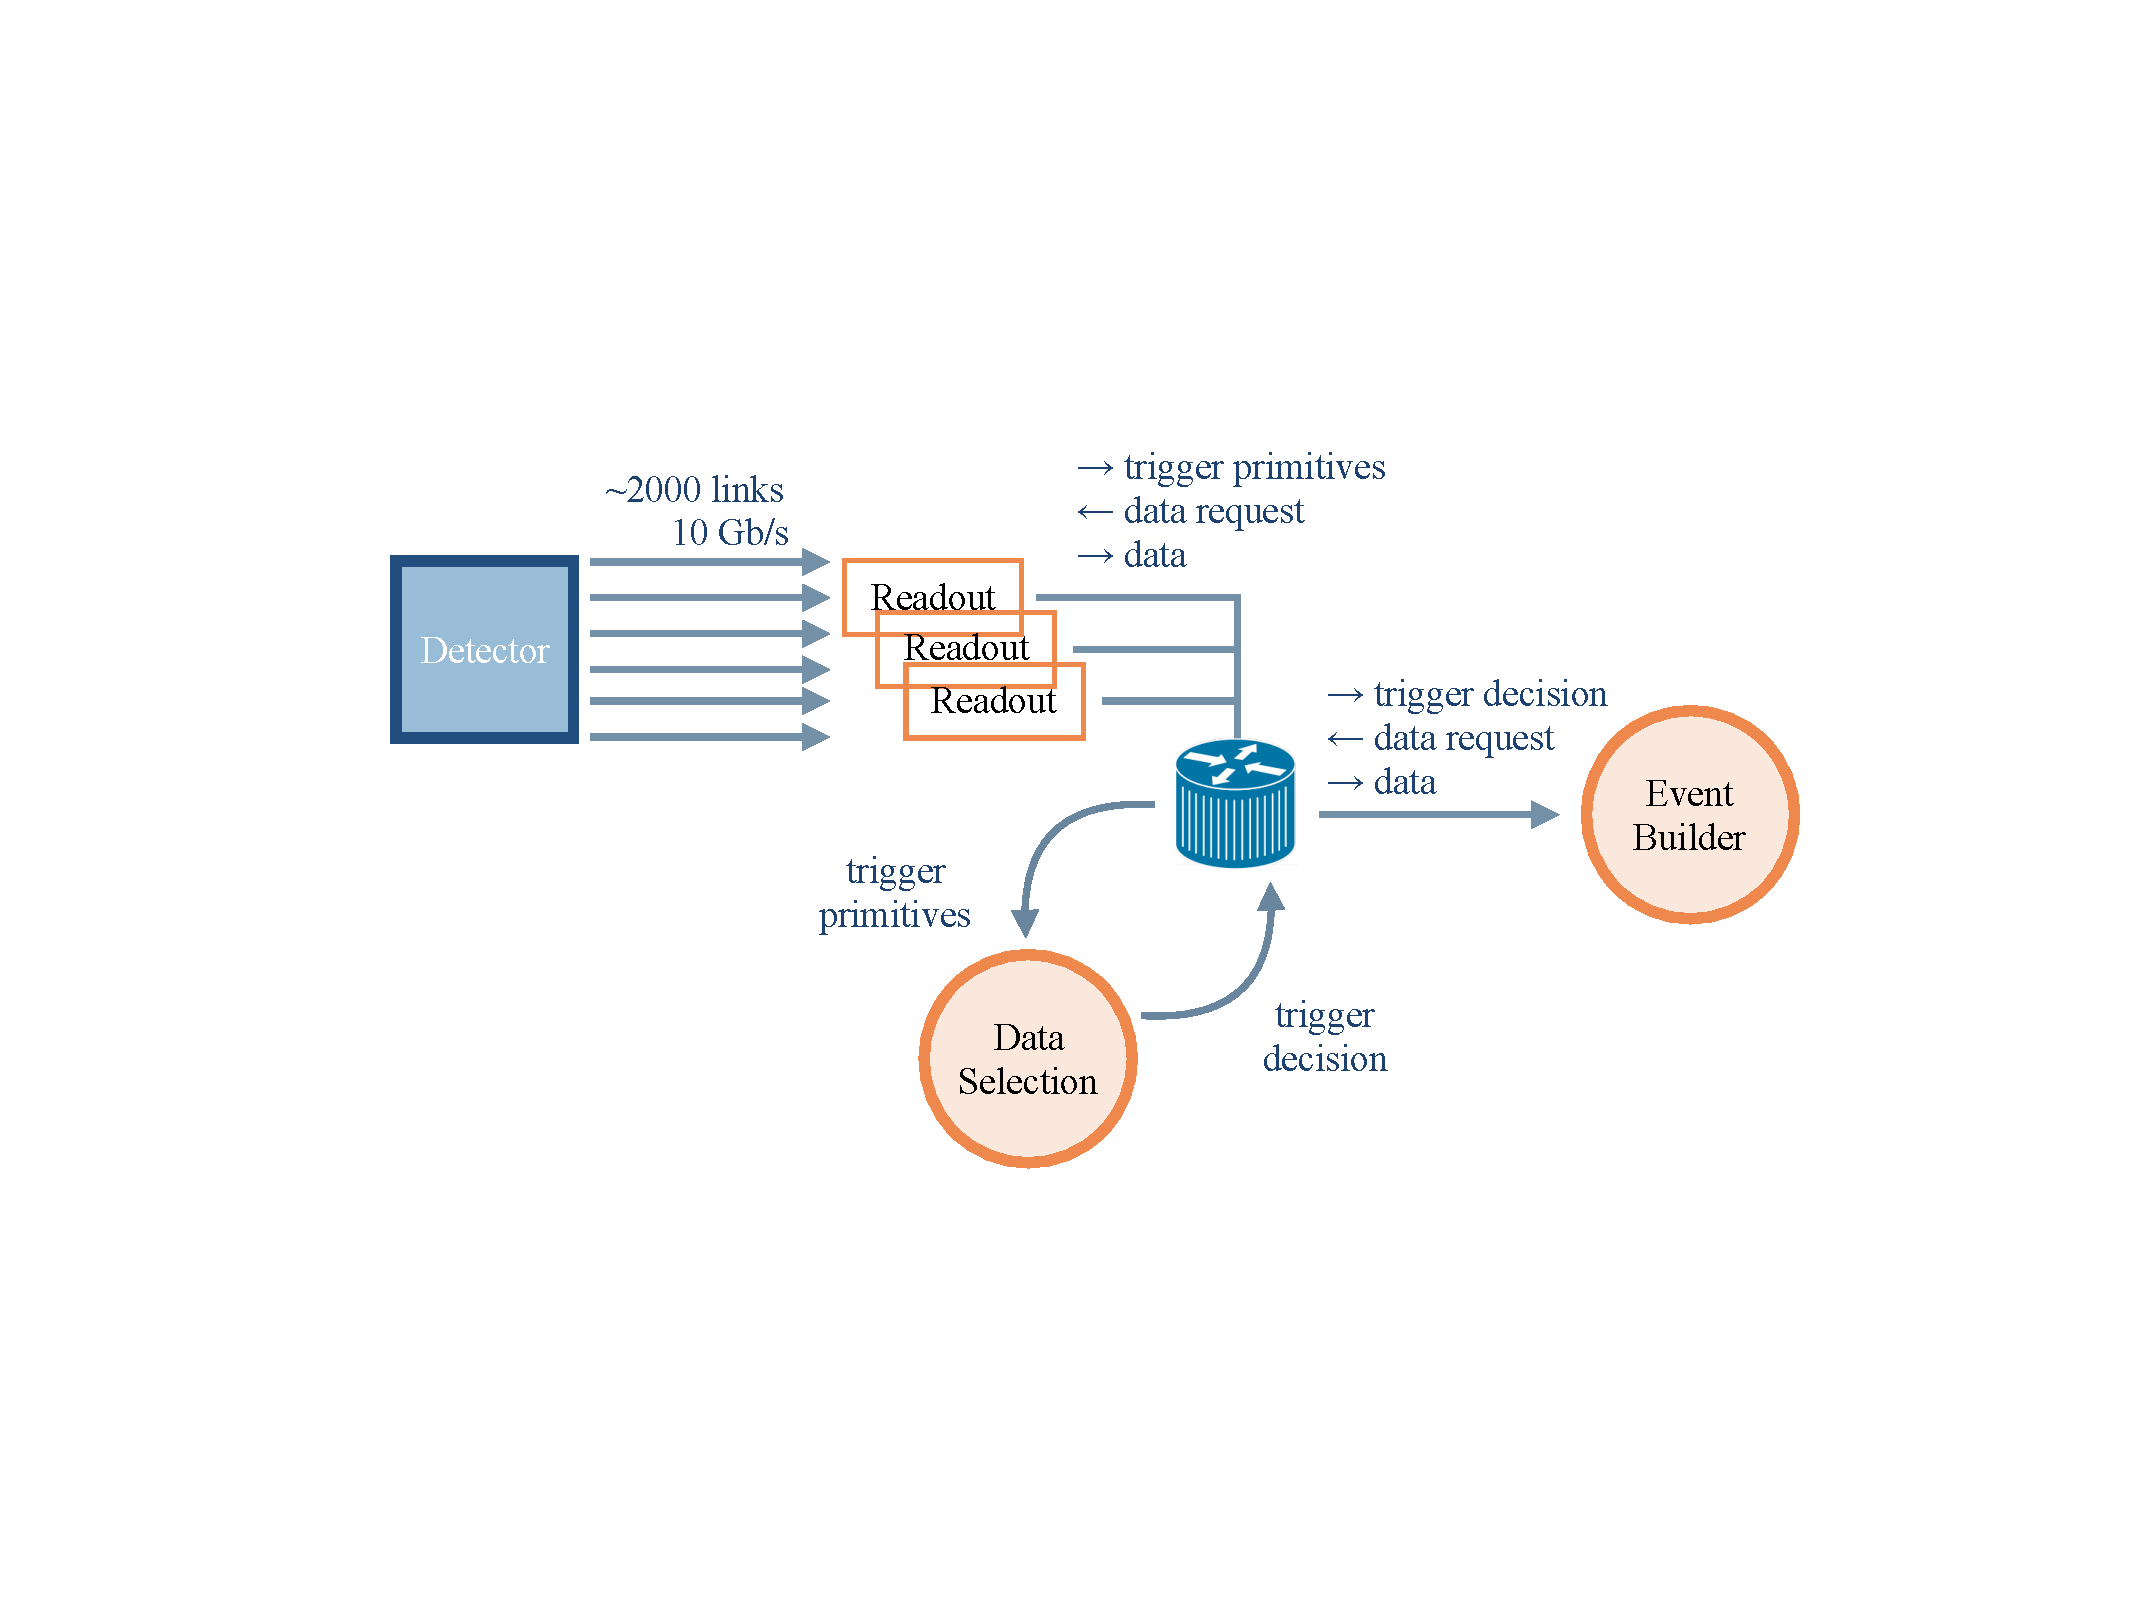
\includegraphics[width=0.8\textwidth]{daq-readout.pdf}
\end{dunefigure}

\begin{dunefigure}{fig:daq:readout-blocks}{\dword{dune} upstream
    \dword{daq} subsystem functional blocks.}
  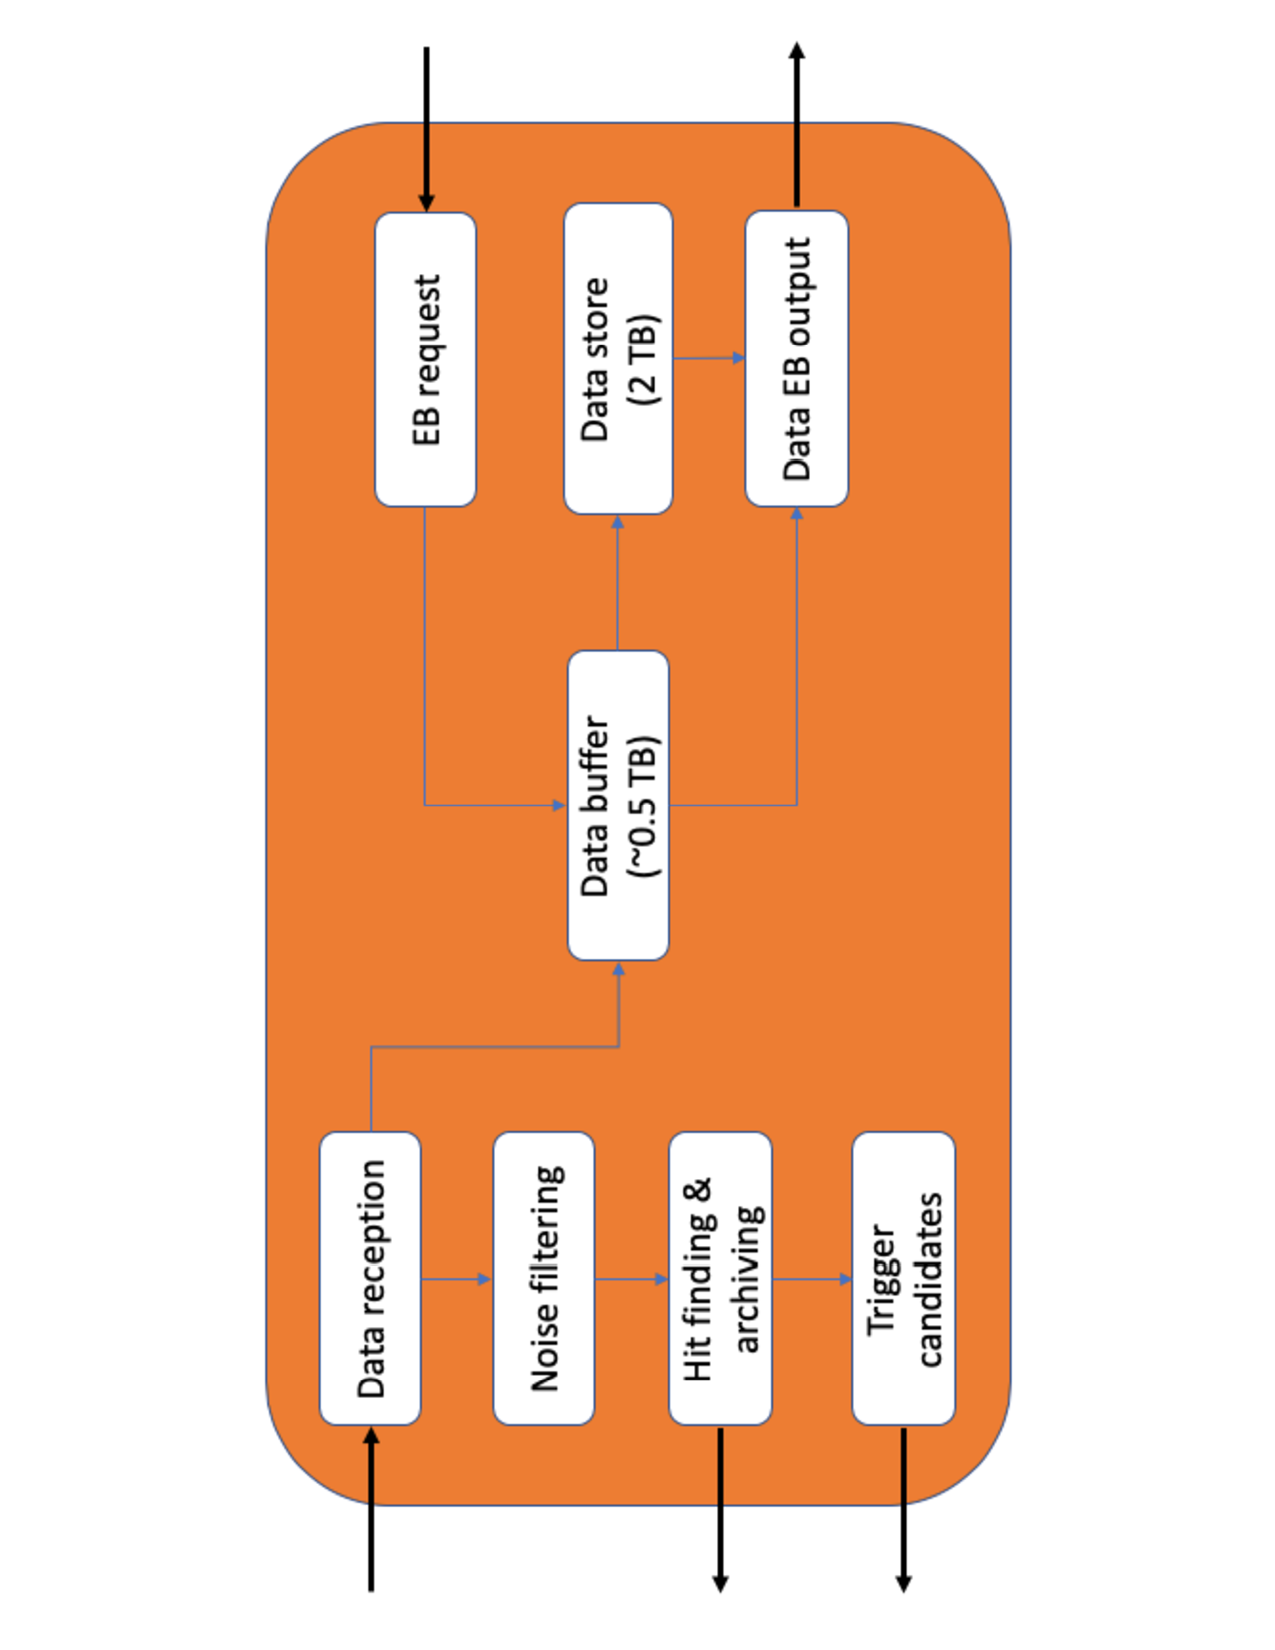
\includegraphics[angle=-90,width=0.8\textwidth]{daq_functional_blocks_upstream.pdf}
\end{dunefigure}

The upstream DAQ system comprises many similar \dword{daqrou}, each connected to
a subset of electronics from a detector module and interfacing with the
\dword{daq} switched network. 
On order one hundred \dword{daqrou} are employed per \dword{detmodule}.
Within one \dword{detmodule}, each are functionally identical and are
responsible receiving the compressed data from the detector electronics,
buffering, decompressing, forming trigger primitives and servicing queries for
portions of the buffered data.
Each RU encompasses a commercial off-the-shelf server that hosts FELIX boards,
and software that collectively form four functional blocks, which work together
as illustrated in Figure~\ref{fig:daq:readout-blocks}, and are itemized below:

\begin{enumerate}
\item Data reception (Section~\ref{sec:daq:upstream-receiver}), facilitated by a FELIX card in the host server
\item Network based I/O (Section~\ref{sec:daq:upstream-io}), facilitated by a commercial off-the-shelf network card
\item Data processing (Section~\ref{sec:daq:upstream-proc}), facilitated by FPGA resources on the FELIX
  card and/or on-host CPU resources, or, in the case of the TPC RU only,
  additional FPGA resources in the form of two dedicated co-processing
  boards (interfacing directly with the FELIX card)
\item Buffering (Section~\ref{sec:daq:upstream-buf}), facilitated by host RAM and SSD, or, in
  the case of the TPC RU only, RAM
  and SSD available on the co-processing boards
\end{enumerate}

Each of these blocks is described below. 
In addition, and like all other \dword{daq} subsystems, the upstream DAQ makes
use of the common software framework for control, configuration, and monitoring
as described in Section~\ref{sec:daq:design-run-control}.

\subsubsection{Data reception}
\label{sec:daq:upstream-receiver}
The physical interface between the dual-phase detector electronics and the \dword{daq} to
transmit data consists of 10 Gbps point-to-point optical links
% {Confirm there is no intervening switch}, yes, there is no switch
carrying messages via standard \dword{udp}.
The number of links per dual-phase  \dword{dune} module is 240 for the charge readout system and 5 for the
the ligh readout system.

To minimize the space and power consumption footprint of the \dword{daq}, 10-20
links are aggregated into \dword{felix} boards hosted in commercial,
off-the-shelf RU computers.
\dword{felix} is an \dword{fpga}-based PCIe board developed initially for ATLAS
and now proposed or already used in several experiments, including
\dword{protodune}. 
Existing firmware has been adopted and is being adapted to ensure
decoding, format checking of incoming data and online decompression and generation of the trigger primitives
%}{What do we say about the required decompression?}
and then to marshal the trigger primitives and compressed data to other blocks of
the upstream DAQ subsystem.

\subsubsection{Network based I/O}
\label{sec:daq:upstream-io}

The upstream DAQ subsystem provides access to the \dword{daqdsn} and \dword{daqbes} through a commercial, off-the-shelf switched network as illustrated in Figure~\ref{fig:daq:readout}).
The network communication protocol is as described in Section~\ref{sec:daq:design-ipc}.
The network I/O is handled by the \dwords{daqrou} via software; dedicated hardware or firmware development is not required.

\subsubsection{Data processing}
\label{sec:daq:upstream-proc}

The data processing functional block consist either as firmware running on the
FPGAs of the FELIX boards or as software running on the RU host computers.
Compression functionality may be offloaded to accelerators such as QAT.
This functional block is ultimately responsible for identifying regions of
interest in the detector at the per-channel level as a function of time (trigger
primitives).

As a preliminary step, data is uncompressed and reformatted to facilitate the
identification of trigger primitives.
The reformatting produces output which retains a data locality matching that of
the detector.
If any digital signal processing is required, such as to suppress excess noise,
it is applied to the sample of channels that provide data for the formation of
trigger primitives.
Finally these regions of interest are located using software algorithms that
maintain a dynamically calculated baseline and noise threshold and search for
periods where the waveform makes an excursion due to signal activity. 
The resulting \dwords{trigprimitive} information packets are made available to
the network by the a service running on the RU.
The primary consumer is the \dword{daqdss} which makes correlations of activity
across the \dword{detmodule} (in channel and time) and ultimately decides
whether and which data is to be saved.


\subsubsection{Buffering}
\label{sec:daq:upstream-buf}

The upstream DAQ system must buffer all detector data for a time sufficient for
the nominal latency for the \dword{daqdss} to issue a trigger command (see
Section~\ref{sec:daq:design-data-selection}) and the \dword{daqbes}
(Section~\ref{sec:daq:design-backend}) to request and receive the corresponding
selected data. 
For the special case of servicing a \dword{snb} trigger, received data must be
continuously buffered for to retain pre-trigger data and a special system must
buffer the extended readout time called for. 
This latter is required to avoid loss of data due to downstream bottlenecks that
would otherwise occur when trying to flow the full data stream for such extended
duration.
Theese two \textit{localized} and \textit{extended} trigger activity patterns
are associated with two rather different time scales and data throughput
metrics, and those collectively dictate the temporary storage technology and
scale. 

The buffering time required to select data associated with a localized trigger
is dominated by processing speed, pipeline depths and network latency.
Some studies must still be performed but initial estimates indicate that the
time buffering time required should not exceed approximately one second. 
When a nominal trigger is used, a \dpreadout block of data must be copied from
the buffer in order to fully capture interesting localized activity without bias
beyond that introduced by the trigger itself.
As the full stream of data must constantly be buffered, a RAM technology is
selected based on providing sufficient throughput, endurance, and capacity. 

Extended triggers present a far more challenging set of buffering requirements.  
Low-energy activity that is associated with a \dword{snb} trigger decision may
exist for as much as \snbpretime prior to the issuing of \dword{snb} trigger
(trigger time).
A second challenge in recording data containing extended activity is that all
channels must be recorded for 100 seconds around the trigger time, and requires
extracting as much as 56 TB 
%}{SP number} 
from the TPC upstream DAQ.
It is not cost effective to design the \dword{daq} to extract such extended data
record in a fully online or streamed fashion.
Thus, additional buffering is provided to catch the temporary backlog of data
that an extended trigger will produce.

The technology and scale of this additional buffering must satisfy several
requirements.  It must accept the full data rate of the detector module (as much as 0.1 TB/s).
%}{SP number} 0.1TB/s is the flux of compressed data from DP (exact number 0.06TB:s)
The data must then reside on nonvolatile media. 
The media must have sufficient capacity and allow for the required extraction
throughput so that it is unlikely to become too occupied to accept yet another
extended data record that arrives before the first can be safely purged.
In terms of capacity, it should be capable of containing several successive
extended data records.
Furthermore, assuming that, on average, a \dword{snb} trigger condition will be
satisfied once per month, the most optimal technology is solid-state devices,
which at the scale required to provide suitable input bandwidth, can provide a
capacity to write the data from several extended activity triggers.
Providing only a modest overhead to normal operations, this data can be
extracted from such storage from the \dword{daq} in well under one hour.
% {More SP'ism.   DP data is substantially smaller}. yes indeed is more than a factor 20 smaller

The data is input to the DAQ in (losslessly) compressed form. 
Although some portion of it much be decompressed prior to having trigger
primitive located, its compressed form will be what is buffered. 
This requires extra complexity in maintaining indices into the buffer that are
``compression aware'' but provides substantial benefits in terms of bandwidths
and capacities given the expected lossless compression factor of ten (for TPC
waveform).
Effort is currently underway to understand the costs and technology involved in
exploiting this benefit.

\subsection{Data Selection}
\label{sec:daq:design-data-selection}

The \dfirst{daqdsn} subsystem is a hierarchical, online, software-based system.
It is responsible for immediate and continuous processing of a substantial
fraction of the entire input data stream from both \dword{cro} and \dword{lro}
sources.
From that input, as well as external inputs provided, for example, by the
accelerator or detector calibration systems, the \dword{daqdss} must form a
\dword{trigdecision} in the form of a \dword{trigcommand} message.
This command summarizes the observed activity that led to the decision. 
The message provides upstream DAQ buffer addresses that are defined in terms of
channel identifiers and time periods.
This command is sent to and then consumed and executed by the back-end DAQ as
described in Section~\ref{sec:daq:design-backend}. 
It is also propagated to the External Trigger Interface and from there it may be
distributed to other \dwords{detmodule} or other detector systems
(e.g. calibration) for consideration.

The \dword{daqdss} must select data associated with calibration signals, as well
as beam interactions, atmospheric neutrinos, rare baryon-number-violating
events, and cosmic ray events that deposit visible energy in excess of 100 MeV
with high efficiency ($>$99\%). 
It must also select data associated with potential galactic \dwords{snb}, with
galactic coverage\footnote{Galactic coverage is defined as efficiency-weighted
  probability of galactic \dword{snb}.} of $>$90\%.
To meet the requirement that the \dword{dune} \dword{fd} maintain
$<$\SI{30}{\peta\byte/\year} to permanent storage, the \dword{daqdss} subsystem
must make \dword{daqdsn} decisions in a way that allows the \dword{daq} system
to reduce its input data by almost three orders of magnitude 
%}{SP number}
without jeopardizing
the above efficiencies.

To meet its requirements, the \dword{daqdss} subsystem design follows a
hierarchical data selection strategy, where low-level decisions are fed forward
into higher-level ones until a module-level trigger is activated. 
The hierarchy is illustrated in Figure~\ref{fig:daq:data-selection-hierarchy}. 
At the lowest level, trigger primitives are formed on a per-channel basis, and
represent, for the baseline design, a ``hit on channel'' activity summary.
Trigger primitives are aggregated into Trigger Candidates, which represent
information associated with higher-level constructs derived from trigger
primitives, for example ``clusters of hits''.
Trigger Candidate information is subsequently used to inform a module-level
trigger decision, which generates a Trigger Command; this takes the form of
either a localized high energy trigger or an extended SNB trigger, and each
prompts readout of an event record.
Post-event-building, further data selection is carried out in the form of
down-selection of event records, through a high level filter.
The data selection strategy is applicable to both \dword{cro} and \dword{lro}
data independently, up to the module level trigger stage, this information can
be combined to form a module level trigger decision.
Data selection design efforts have taken the approach of validating and
demonstrating a solely \dword{cro}-based data selection, with the expectation that
optical data selection can only augment data selection capabilities and efficiencies.

The subsystem structure is illustrated in Figure~\ref{fig:daq:data-selection}.
The structure reflects the three stages of \dword{daqdsn}: (1) low level
trigger, which consists of \dword{trigprimitive} generation and subsequent
\dword{trigcandidate} generation; (2) module level trigger; and (3) high level
filter.
Each stage is described in subsequent sections.
An additional subsystem component is the external trigger interface, which
serves as a common interface for the module level trigger of each of the FD
\dwords{detmodule} and between the module level trigger and other systems
(e.g.,~calibration, accelerator and timing system) within a single
\dword{detmodule}.
After sufficient confirmation of quality the external trigger interface also
sends \dword{snb} triggers to global coincidence trigger recipients such as
\dword{snews}~\cite{snews}.

\begin{dunefigure}{fig:daq:data-selection-hierarchy}{Data Selection
    strategy and hierarchy.}
  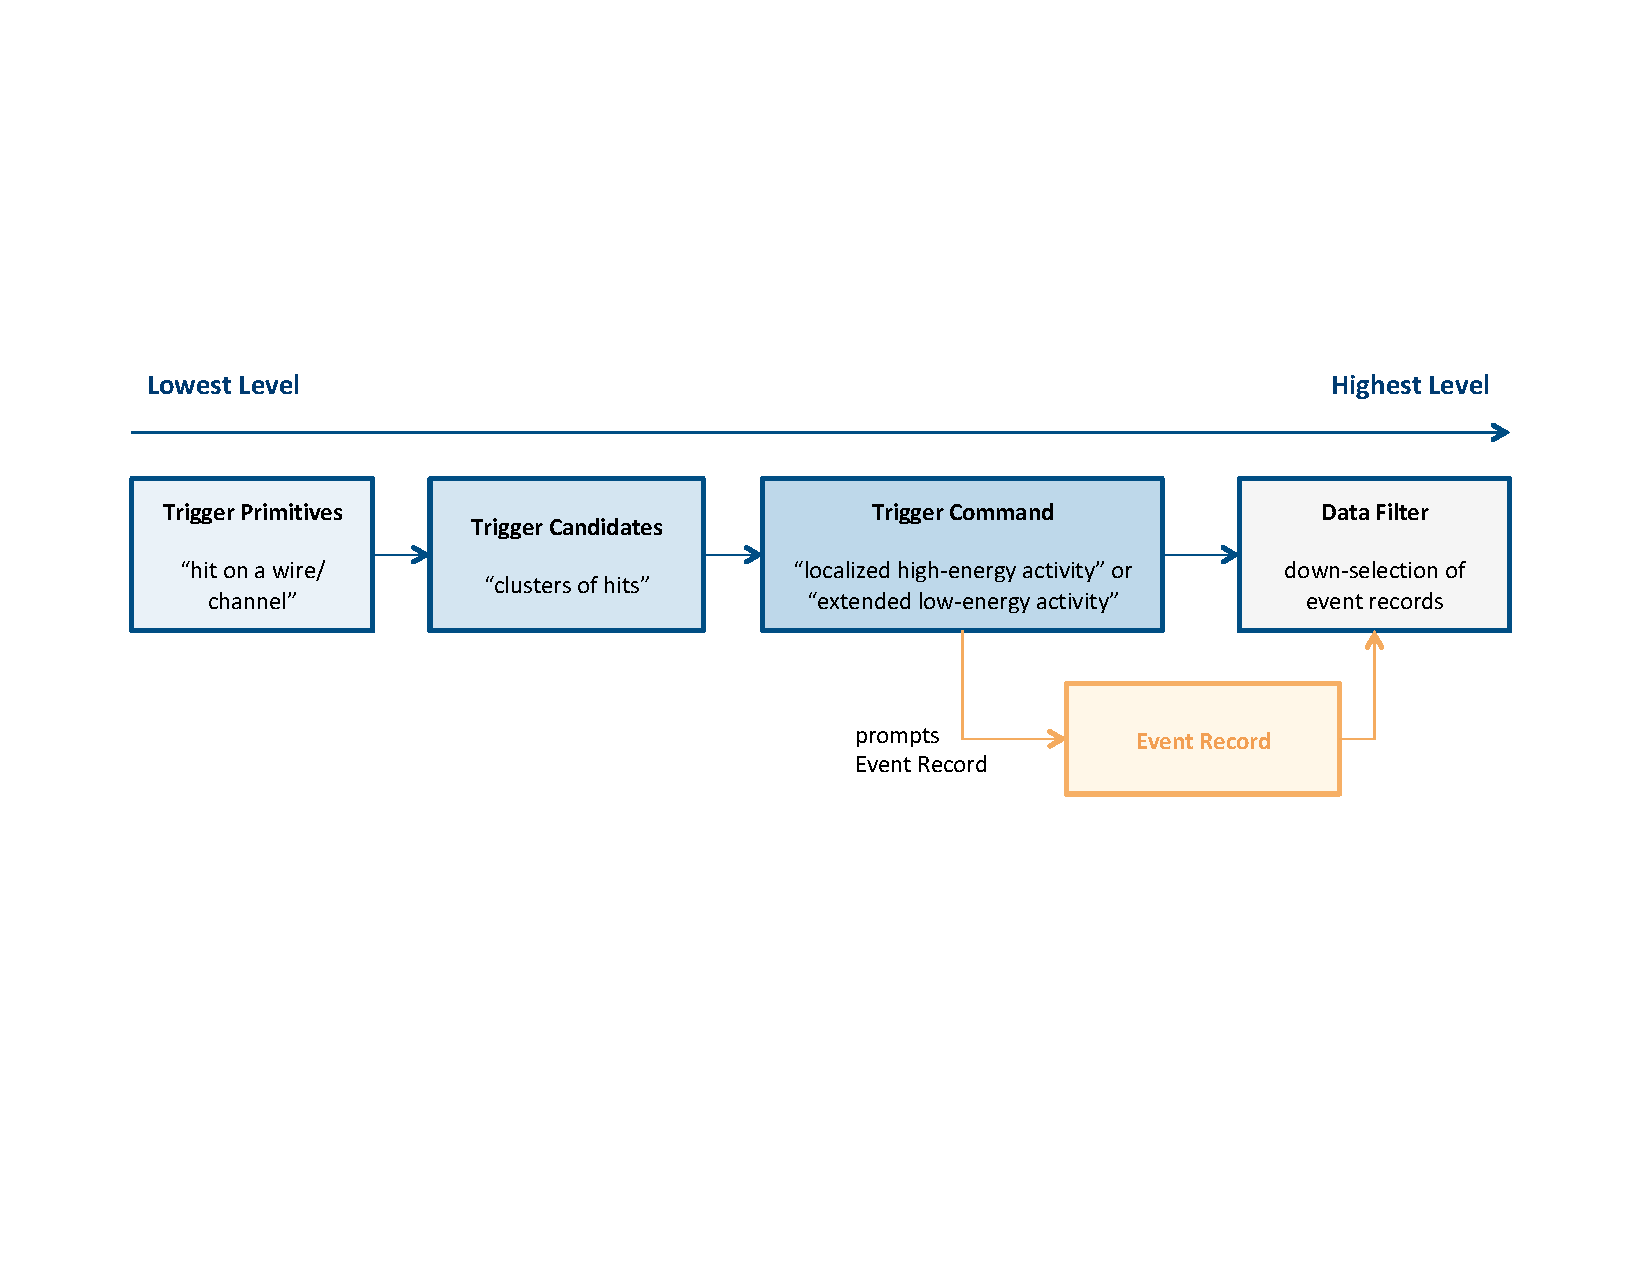
\includegraphics[width=0.9\textwidth, clip, trim=0cm 7cm 0cm 6cm]{DS_hierarchy.pdf}
\end{dunefigure}

\begin{dunefigure}{fig:daq:data-selection}{Block diagram of \dword{dune} \dword{daq}
    \dword{daqdsn} subsystem, illustrating hierarchical structure of
    subsystem design, and subsystem functionality.}
  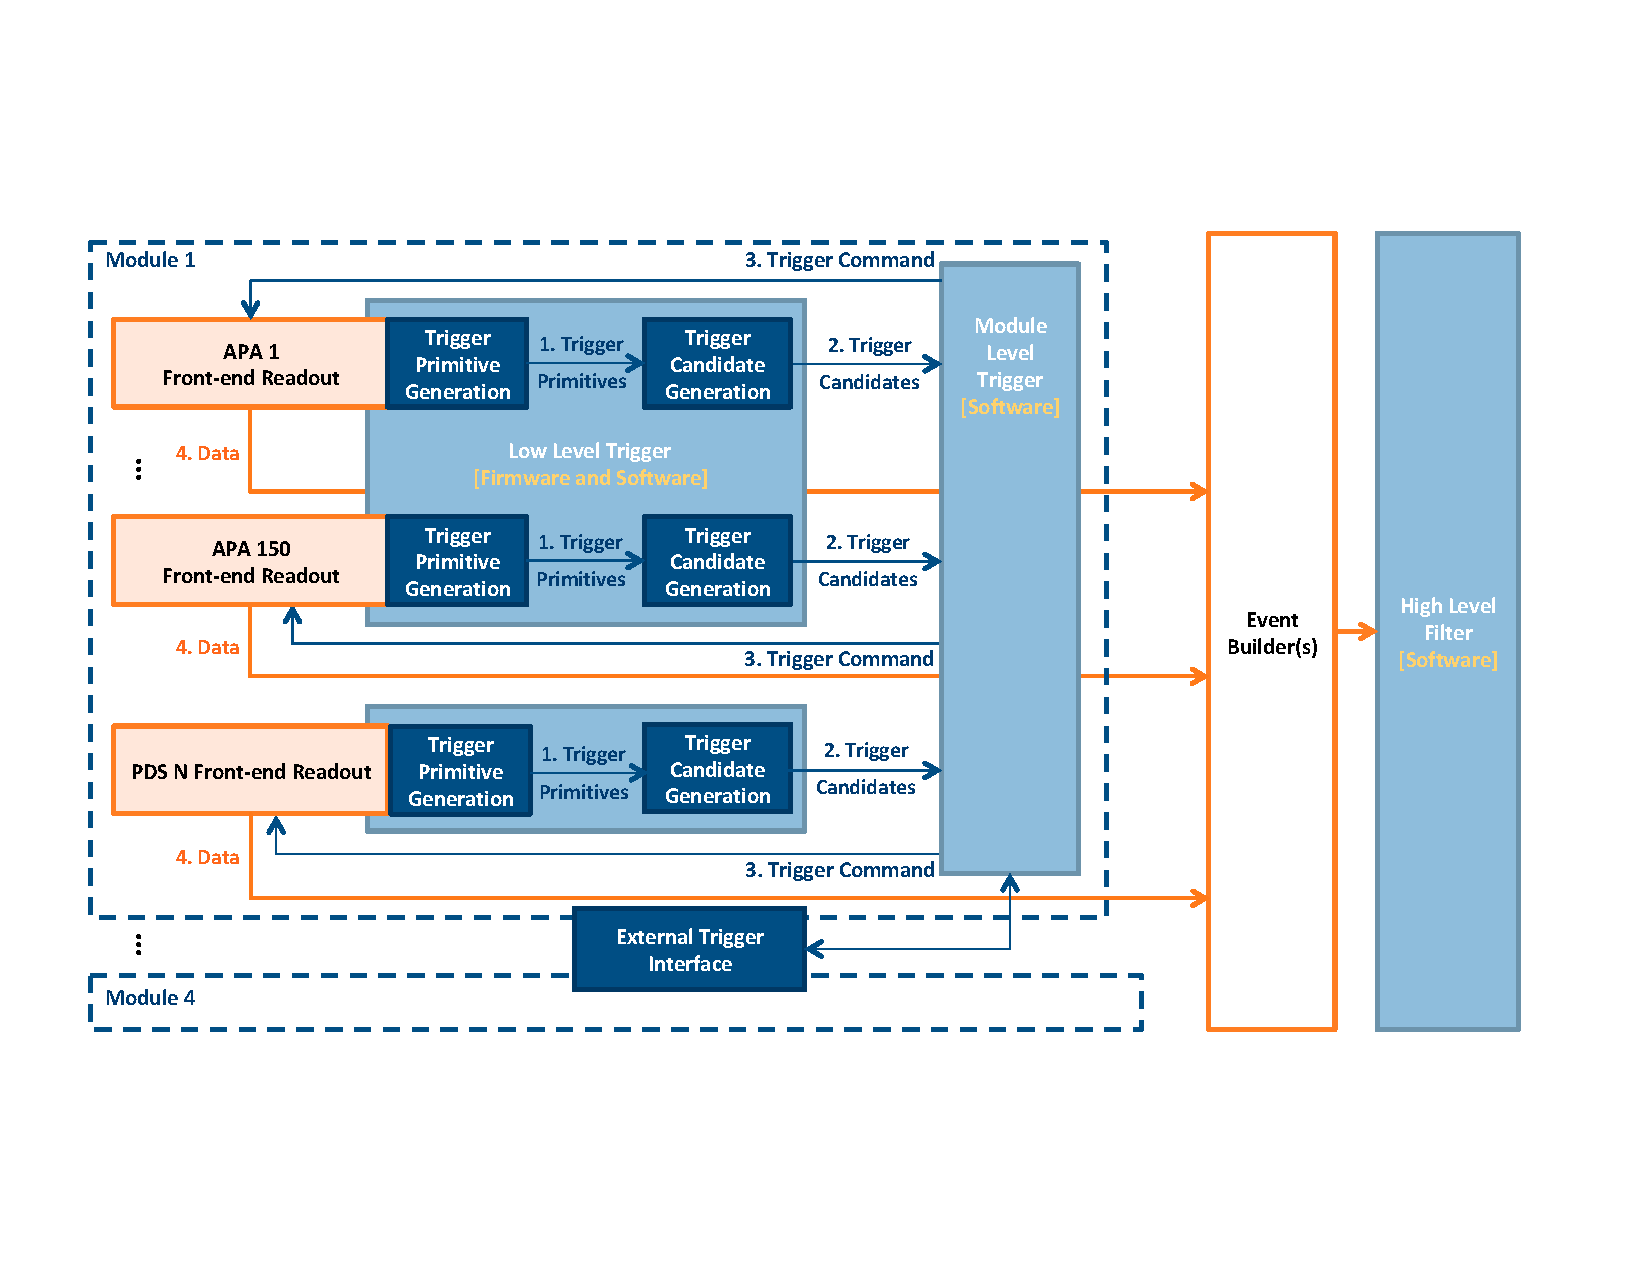
\includegraphics[width=0.95\textwidth, trim=0 2cm 0 0]{DS_summary_2.pdf}
\end{dunefigure}

To facilitate partitioning, the \dword{daqdsn} subsystem will be able to be
instantiated multiple times, and multiple instances will be able to operate in
parallel.
Within any given partition, the \dword{daqdsn} subsystem will also be informed
and aware of current detector configuration and conditions and apply certain
masks and mapping on subdetectors or their fragments in its decision making.
This information is delivered to the \dword{daqdss} from the \dword{daqccm}
system.

Ultimately, each \dword{trigdecision} culminates in a command executed by the
\dword{daqbes}. 
This command contains all the logical detector addresses and time ranges
required such that an \dword{eb} may properly query the \dword{daqfbi} and
finally collect and output the corresponding detector and trigger data.
To avoid duplication of data records associated with trigger commands that
overlap in readout record ``space'', the \dword{daqdsn} system must also
time-order and prioritize trigger decisions.
The details for forming this command are described next and the operation of the
\dword{daqbes} is described in Section~\ref{sec:daq:design-backend}.

The first stage of DUNE FD operations will have two general classes of trigger
decisions that are categorized in terms of the distribution of activity
in time and channel (mapped to physical) space from which they are derived: 
\begin{itemize}
\item Any given far detector module will make a trigger decision with $>$99\%
  efficiency for any given particle type (electron, muon, photon, etc.) 
  which deposits more than 100 MeV of visible energy in a locally confined
  region (e.g.~a single or two neighboring \dwords{cro}). To achieve this goal,
  data selection algorithms are targeting a trigger threshold of \hlfix{10 MeV
  }{This has not yet been studied for DP} in visible energy, ensuring $>99$\%
  efficiency or better at 100 MeV. 
  This type of trigger is referred to as localized high energy trigger.
\item Localized activity associated with low deposited energy (as low as below
  10 MeV) serves as input to a different type of trigger, referred to as
  extended low energy trigger, which is intended for capturing supernova
  neutrino bursts.
  It differs from localized high energy triggers in that it considers the
  coincidence of localized activity across the entire module, and over an
  integration period of up to 10 seconds.
\end{itemize}
Each trigger type furthermore prompts readout of the entire module but over
significantly different time ranges: localized triggers prompt readout of
\dpreadout; extended triggers prompt readout of \snbtime. 

Viable algorithms for the low level and module level trigger already exist,
including algorithms for a module level supernova burst trigger, and it has been
demonstrated offline that the resulting efficiencies meet the DUNE  requirements
%{Strictly speaking, only with SP.    Is it acceptable to stretch this to DP?}, yes since the algorithms for the collection view can be applied similarly 
~\cite{xx}.
On the other hand, the pipelines of processing required for \dword{daqdsn} can
be executed using different firmware and software implementations.
Development is actively ongoing to demonstrate and compare performance of
different implementations.
In satisfying the philosophy and strategies of the \dword{daq} design, there is
built-in flexibility in defining whether each element of a pipeline executes on
FPGA
%}{Does this still hold true for DP?}, yes, the decompression and search for trigger primitives should preferably happen in the FPGA of the felix card
CPU, GPU, or, in principle, some other future hardware architecture.
A purely CPU implementation of data selection has been the subject of
successful, ongoing demonstration tests at ProtoDUNE.
An FPGA implementation of the lowest level of data selection (specifically,
trigger primitive generation), however, is possible within the upstream DAQ
design, and offers an opportunity to reduce CPU costs as well as costs
associated with power consumption during detector operations.
It is therefore the subject of ongoing development at ProtoDUNE.

\subsubsection{Low Level Trigger: Trigger Primitive Generation}
\label{sec:daq:design-trigger-primitives}

A \dword{trigprimitive} is defined nominally on a per-channel basis.
In the case of \dword{cro} input, it is identified as a waveform rising above
some noise-driven threshold for some minimum period of time (here called a
``hit'').
A \dword{trigprimitive} takes the form of an information packet that summarizes
the above-threshold waveform information in terms of its threshold crossing
times and statistical measures of its \dword{adc} samples. 
In addition, these packets carry a flag indicating the occurrence of any
failures or other exceptional behavior during \dword{trigprimitive} processing.
\Dwords{trigprimitive} are produced via software running in the upstream DAQ RUs
as described in Section~\ref{sec:daq:design-upstream}.

Algorithms for generating \dwords{trigprimitive} are under continual
\hlfix{development}{Technically, SP only, but should be easier for
  DP.}~\cite{docid-11275}.
Nominally, trigger primitive generation proceeds by establishing a waveform
baseline for a given channel, subtracting this baseline from each sample,
maintaining a measure of the noise, and searching for the waveform to cross a
threshold defined in terms of the noise level.
This thredhold crossing represents a ``hit''. 
Such algorithms (see, e.g.~\cite{docid-11236}) have been validated using both
Monte Carlo simulations and real data from \dword{protodune}. 
Trigger primitive generation performance is summarized in
Section~\ref{sec:daq:design-validation}.

The format and schema of \dwords{trigprimitive} are subject to further
optimization, as they are further tightly coupled with the generation of trigger
candidates, discussed in the following subsection.
Nominally, each trigger primitive comprises the channel address (32 bit), hit
start time (64 bit), the time over threshold (16 bit), the integral ADC value
(32 bit), an error flag (16 bit), and possibly also the waveform peak (12 bit)
associated with the hit. 
As such, 20-22 bytes provides a generous data representation of
\dword{trigprimitive} information. 
The \dword{trigprimitive} rate will be dominated by the rate of decay of
naturally occurring $^{39}$Ar, which is about \SI{10}{\mega\hertz} per module.
This leads to a detector module aggregate rate of \SI{200}{\mega\byte/\second}.
The subsequent stage of the \dword{daqdsn} must continuously absorb and process
this rate providing trigger candidates as described next.

\subsubsection{Low Level Trigger: Trigger Candidate Generation}

At the trigger candidate generation stage of the low level trigger,
\dwords{trigprimitive} from individual, contiguous fragments of the detector
module are cross-channel and -time correlated, and further selection criteria
are applied.
This may result in the output of trigger candidates. 
More specifically, once activity is localized in time and channel (``space'') it
is possible to apply a rough energy-based threshold based on the combined
metrics carried by the cross-correlated \dwords{trigprimitive}; satisfying this
criteria defines a trigger candidate. 

A trigger candidate packet carries information about all the trigger
primitives that were used in its formation. 
In particular, it provides a measure of the total activity represented
by these primitives, as well as a measure of their collective time and channel
location and extent within the module.
These measures are used downstream by the module level trigger, 
as described more in the next section.

While the selection applied in the previous stage (trigger primitive generation)
is driven by a measure of noise, at trigger candidate generation stage it is
driven by background activity.  
In particular, the very high rate, low energy $^{39}$Ar decays are expected to
dominate trigger candidate rates, followed by activity from the $^{42}$Ar decay
chain.
Nominally, individual candidates, or groups of candidates nearby in detector
space in time, with measures of energy greater than these two types of decays,
will be passed to the module level trigger. 

This stage of data selection is implemented in O(100) CPU servers, which receive
the trigger primitive stream from the upstream DAQ and distribute trigger
candidates to the module level trigger stage, described next, via the 10 Gbps
DAQ network.
Studies are underway to demonstrate CPU resource utilization and latency, as are
efforts to demonstrate online trigger candidate generation at
ProtoDUNE.
%{True for DP?}. yes, see discussion with Giovanna at the May 2019 DUNE meeting and text in next paragraphs
Trigger candidate generation performance is summarized in
Section~\ref{sec:daq:design-validation}. 


\subsubsection{Module Level Trigger}

Data selection is further facilitated as trigger candidates are consumed by the
module level trigger in order to form the ultimate trigger decision which
prompts the readout of event records. 
The physical (channel and time) location, extent as well as the energy measure
of the candidates are used at this stage to categorize the activity in terms of
a localized high energy trigger or an extended low energy trigger. 
Specifically, $\mathcal{N}$ isolated, low energy candidates found in coincidence
over the integration period of up to 10 seconds across the full
\dword{detmodule} indicate the latter; individual high energy candidates, found
otherwise, indicate the former.

When a particular condition in a category is satisfied, the trigger decision is
made and a trigger command is formed. 
The trigger command packet includes information of the candidates (and
primitives) that were used to form it. 
The decision also provides direction as to what set of detector subcomponents
are to be read out and over what time period. 
As described at the start of this section, localized triggers will instruct the
readout of the entire detector module for a period equal to \dpreadout.
Extended triggers (\dword{snb}) will instruct the readout of much longer period
of \snbtime.

The module level trigger provides its produced trigger commands to the
\dfirst{daqbes} for the detector module, specifically the \dword{daqdfo} is
their receiver.
This in turn dispatches the command to an \dword{eb} for execution as described
in Section~\ref{sec:daq:design-backend}.
The entire data selection chain as well as resulting query for data from the
\dword{daqfbi} must be accomplished promptly compared to the depth of the
upstream DAQ buffer.

The module level trigger is implemented in O(1) CPU server (with 100\%
redundancy), which receives the trigger candidate stream from the lower level
trigger stage of the data selection and distributes trigger commands to the
backend DAQ via the 10 Gbps DAQ network.
Studies are underway to demonstrate CPU resource utilization and latency, as are
efforts to demonstrate online trigger command generation at ProtoDUNE.
Trigger command generation performance is summarized in
Section~\ref{sec:daq:design-validation}.

\subsubsection{External Trigger Interface}

The external trigger interface provides proxy to exchange messages between
module level triggers of the far detector modules, elements of the calibration
system, and sources and sinks of trigger information in the outside world
(external to the far detector).
\hlfix{It is also responsible for correlating system timing with trigger
  information.}{What does this mean?}

Trigger commands generated by the module level trigger are also sent, via the
external trigger interface, to other detector modules, and vice versa.
This is needed in order to allow for cross-module coincidences to be formed and
thus produce an overall lower threshold for capturing potential \dword{snb}
occurrences. 
The external trigger interface also forwards \dword{snb} trigger commands, after
suitable quality confirmation, to external recipients such as \dword{snews}.

In addition to accepting cross-module triggers via the external trigger logic
unit, the module level trigger must take inputs from out-of-band sources such as
needed for beam, calibration, or random triggering. \hlfix{These inputs are all
  received via the external trigger interface, where they are correlated against
  the global clock (derived from the timing system); the global timestamp of
  each input is forwarded to the module level trigger.}{This seems to confuse
  real and data time. 
  It needs more clarity (also in SP section).}
The module level trigger may also issue timestamps (in anticipation of beam
triggers, for example) for calibration signals.
Those are forwarded to the timing subsystem via the external trigger interface,
and get further distributed to calibration systems by the timing subsystem (see
Section~\ref{sec:daq:design-timing}). 

% The external trigger interface is implemented in O(1) CPU server (with 100\%
% redundancy), which hosts a number of White Rabbit node cards for
% receiving accelerator and other timing inputs.

\subsubsection{High Level Filter}
\label{sec:daq:design-data-reduction}

The last processing stage in the \dword{daqdsn} subsystem is the
high level filter, which resides in the back-end part of the \dword{daq}.
The high level filter acts on triggered, read out, and aggregated data,
produced by an \dword{eb}. 
It therefore serves primarily to down-select and thus
limit the total triggered data rate to offline, thereby keeping %. This allows to keep
efficiency high in collecting information on activities of interest
while minimizing selection and content bias, and reducing the output data
rate. It may do so via 
further filtering, lossy data reduction, and/or further event
classification. As it benefits from a longer latency (time between
$\sim$Hz-level built event records), it can accommodate a higher level of
sophistication in algorithms for \dword{daqdsn} decisions.

More specifically, the high level filter may further reduce the rate of data
saved to final output storage by applying refined selection criteria which may
otherwise be prohibitive to apply to the pre-trigger data stream.
For example, instrumentally-generated signals (e.g.~correlated noise) may
produce trigger candidates that can not be rejected by the module level trigger
and if left unmitigated may lead to an undesirably high output data rate. 
Post processing the triggered data may allow reducing this unwanted
contamination.
Furthermore, it can also reduce the triggered data set by further identifying
and localizing interesting activity.
A likely candidate hardware implementation of this level of \dword{daqdsn} is a
GPU-based system residing on surface at SURF.

To fully understand how much and what type of data reduction may be beneficial,
simulation studies are ongoing \citedocdb{xx} and will necessarily have to be
validated with initial data analysis after first DUNE \dword{fd} operation.
Development efforts are also being carried out to determine the scale of
processing required by the \dword{fd}.


\subsection{Back-end DAQ}
\label{sec:daq:design-backend}

The functionality of the \dfirst{daqbes} is represented by the ``Event Builder''
and ``Data Flow Orchestrator'' in Figure~\ref{fig:daq:layout} or the ``Output''
circle in Figure~\ref{fig:daq-conceptual-overview}. 
It accepts trigger commands produced by the \dfirst{daqdss} as described in
Section~\ref{sec:daq:design-data-selection}. 
It queries the upstream DAQ buffers and accepts returned data as described in
Section~\ref{sec:daq:design-upstream}. 
Finally, it records trigger commands and the corresponding data in the form of
``event records'' to the output storage buffer, from which the data is
transferred to offline.

\subsubsection{Dataflow Orchestration}

To minimize the latency in the readout of the data from the Upstream DAQ
buffers, the back-end DAQ will support parallel readout of event records into a
pool of Event Builder processes. 
This asynchronous, parallel readout will be coordinated by a dataflow
orchestrator (DFO). 
Its operation is illustrated in Figure~\ref{fig:daq:backend} and is discussed
here:

\begin{dunefigure}{fig:daq:backend}{Illustration of \dword{dune} \dword{daq} back-end operation.}
  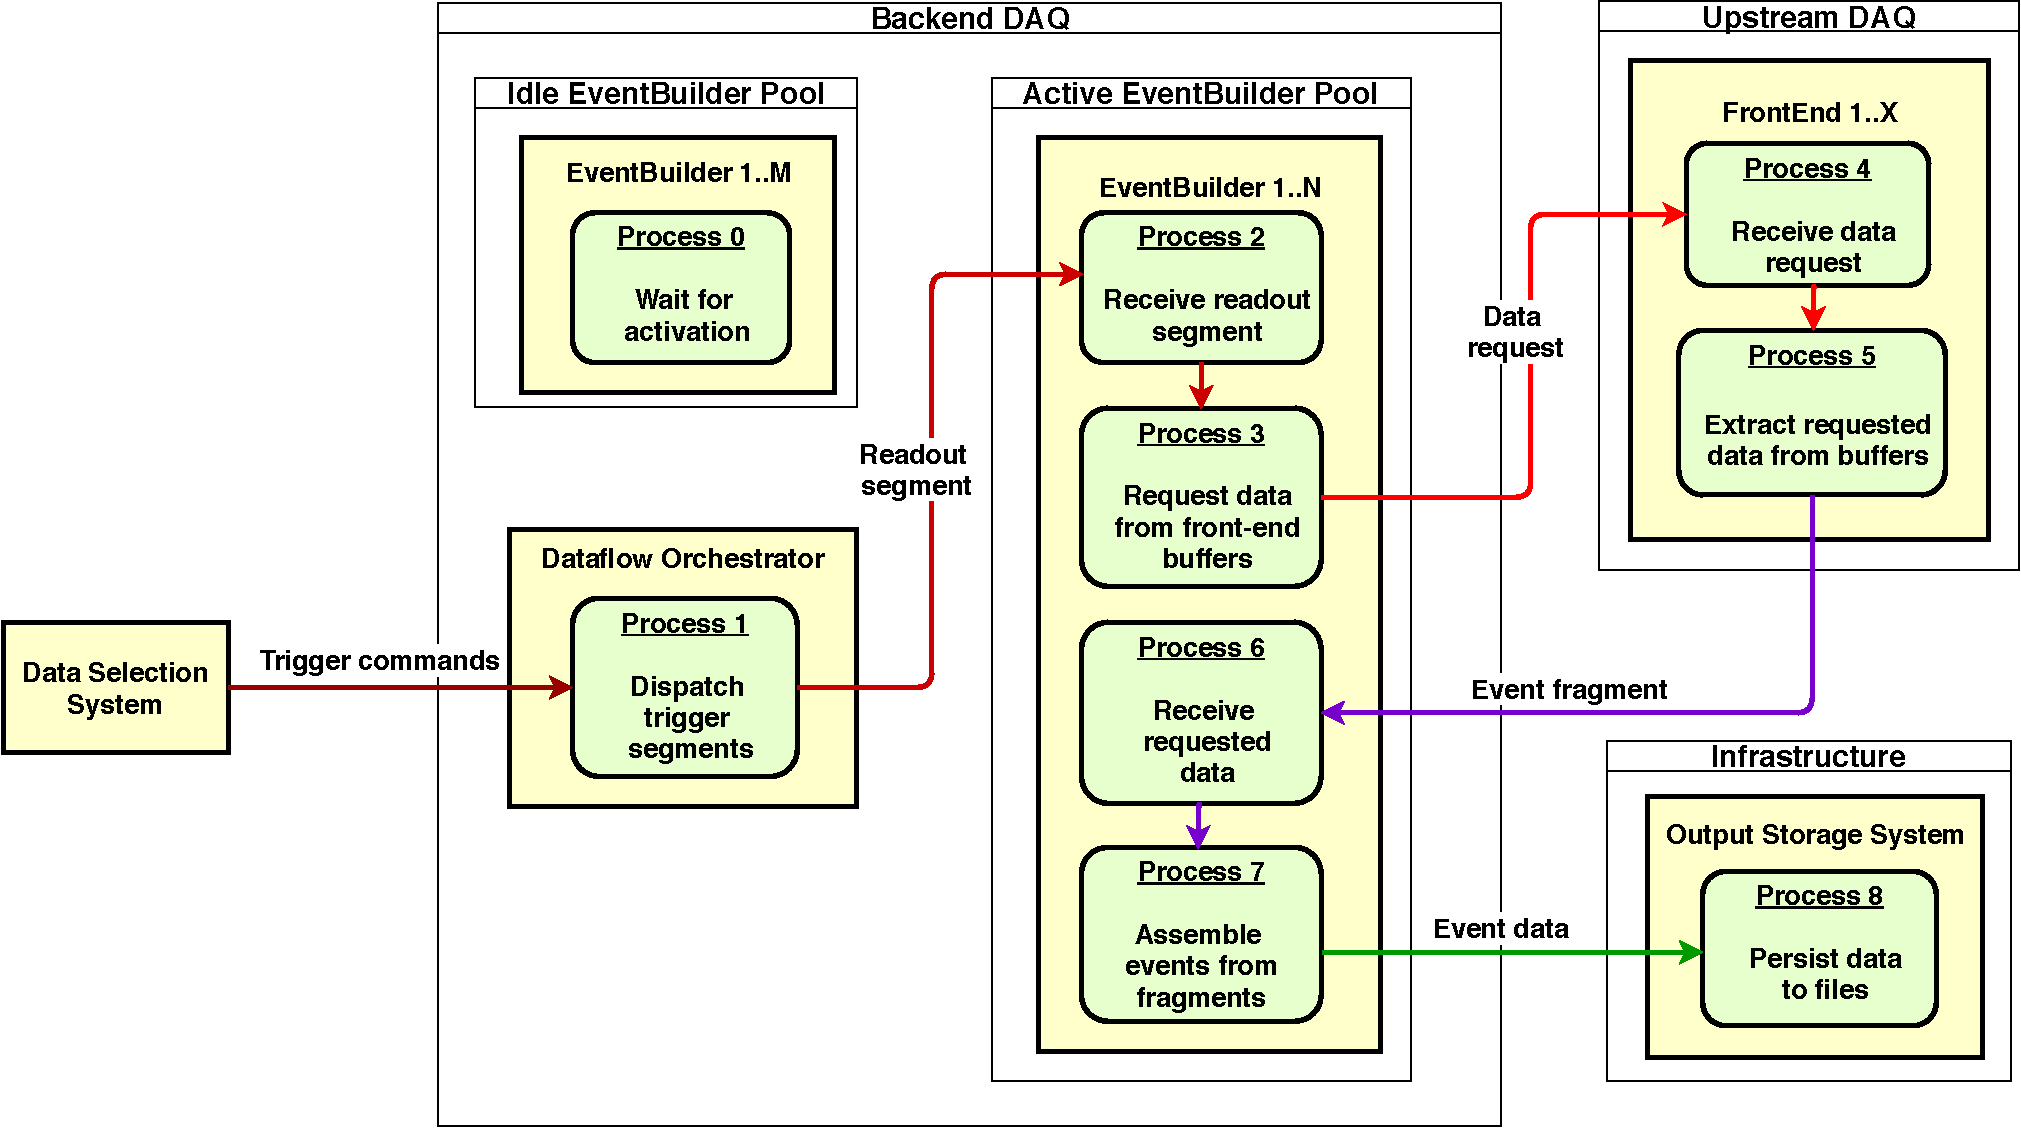
\includegraphics[width=0.8\textwidth]{daq-backend.pdf}
\end{dunefigure}

\begin{itemize}
\item \dword{daqdfo} accepts a time ordered stream of \dwords{trigcommand} and
  dispatches each for execution possibly by first splitting up each command into
  one or more contiguous segments.
\item Each segment will then be dispatched to an \dword{eb} process as described
  in Section~\ref{sec:daq:design-event-builder} for execution.
\item Execution entails interpreting the trigger command segment and querying
  the appropriate \dword{fe} buffer interfaces to request data from the period
  of time. 
\item Requests and their replies may be sent synchronously, and replies are
  expected even if data has already been purged from the \dword{fe} buffer.
  (In that case, an error message would be sent out.)
\item The data received may then undergo processing and aggregation
  until finally it is saved to one or more files on the output storage
  system before it is transferred offline.
\end{itemize}


\subsubsection{Event builder}
\label{sec:daq:design-event-builder}

The \dword{daq} back-end subsystem will provide the instances of the \dfirst{eb}
most likely as \textit{artDAQ}~\cite{artdaq} components of the same name.
As described above, each EB instance will request selected data from the
appropriate \dfirst{daqfbi}, as addressed by a received trigger command. 
An \dword{eb} will aggregate the selected data and potentially apply processing
and reduction (Section~\ref{sec:daq:design-data-reduction}) as well as monitor
its quality while in flight.
Finally it will record the resulting data to the output storage system.
The final output files shall use data schema and file formats as described in
Section~\ref{sec:daq:design-data-model}.


\subsubsection{Data Quality Monitoring}
\label{sec:daq:design-data-quality}

Section~\ref{sec:daq:design:ccm:monitoring} describes a monitoring system for
the \dword{daqccm} subsystems. 
Monitoring the quality of the information held in the detector data itself is
critical to promptly responding to unexpected conditions and maximizing the
quality of acquired data. 
A \dword{daq} \dfirst{dqm} will be developed (including necessary
infrastructure, visualization, and algorithms), which will process a subset of
detector data in order to provide prompt feedback to the detector operators. 
This system will be designed to allow it to evolve as the detector and its data
is understood during commissioning and early operation and to cope with any
evolution of detector conditions.
It is likely that many of the software modules developed by the offline effort
will be reused in the DQM.

\subsubsection{Output Buffer}

The output buffer system is a hardware resource provided by \dword{daq} and used
offline by \dword{dune}. 
It has two primary purposes. 
First, the buffer decouples the production of event data from the transfer of
that data from the far site to archival storage.
Second, it provides local storage sufficient for uninterrupted \dword{daq}
operation in the unlikely event that the connection between the \dword{fd} and
the Internet is lost. 
A capacity of approximately \SI{0.5}{\peta\byte} is envisioned, sufficient to
service the entire \dword{fd}.
This corresponds to one week's worth of data at nominal data rates.
Based on prior experience of the consortium with unusual losses of connectivity
at other far detector experiment sites, this is a conservative storage capacity
value.

\subsubsection{Data Model}
\label{sec:daq:design-data-model}
\fixme{Add reference to live document. Georgia}

\metainfo{Describe the data model. 
  This isn't a strict schema just things like how various parts of the
  detector readout map to files, etc.}



\subsection{Control, Configuration, and Monitoring}
\label{sec:daq:design-run-control}

The \dfirst{daqccm} subsystem, illustrated in Figure~\ref{fig:daq-ccm-subsys},
encompasses, as its name suggests, the software needed to control, configure,
and monitor the rest of the \dword{daq}, as well as itself. 
It provides a center for the highly distributed \dword{daq} components, allowing
them to be treated and managed as a single, coherent system. 
Figure~\ref{fig:daq-conceptual-overview} shows the central role of the
\dword{daqccm} within the complete \dword{daq} system.
The following sections describe each of the three \dword{daqccm} subsystems. 

\begin{dunefigure}{fig:daq-ccm-subsys}{Main interaction among the three \dword{daqccm} subsystems.}
  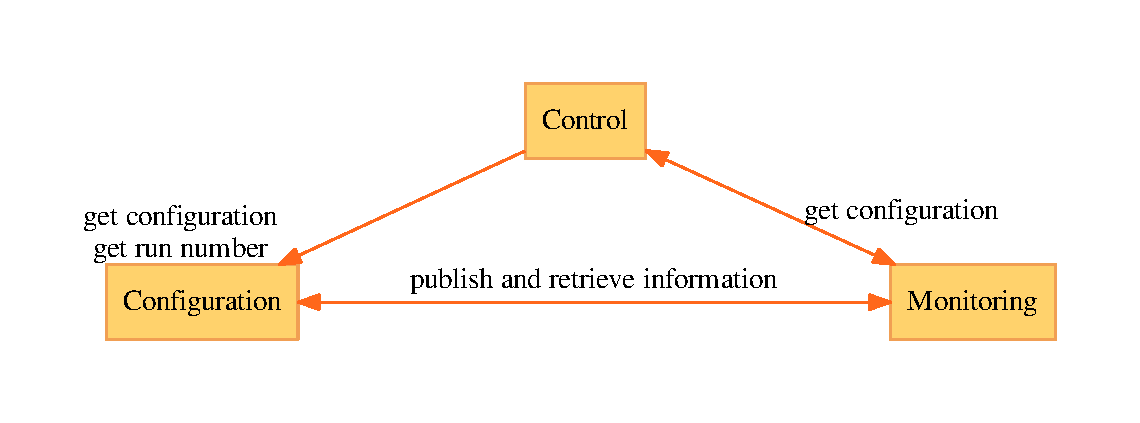
\includegraphics[width=0.8\textwidth]{daq-ccm-subsys.pdf}
\end{dunefigure}

\subsubsection{Control}
\label{sec:daq:design:ccm:control}


The \dword{daq} control subsystem actively manages \dword{daq} software process
lifetimes, asserts access control policies, executes commands, initiates
configuration changes, detects and handles exceptions, and provides an interface
for human operators.

\begin{dunefigure}{fig:daq-ccm-control}{Roles and services that compose the \dword{daq} control subsystem.}
  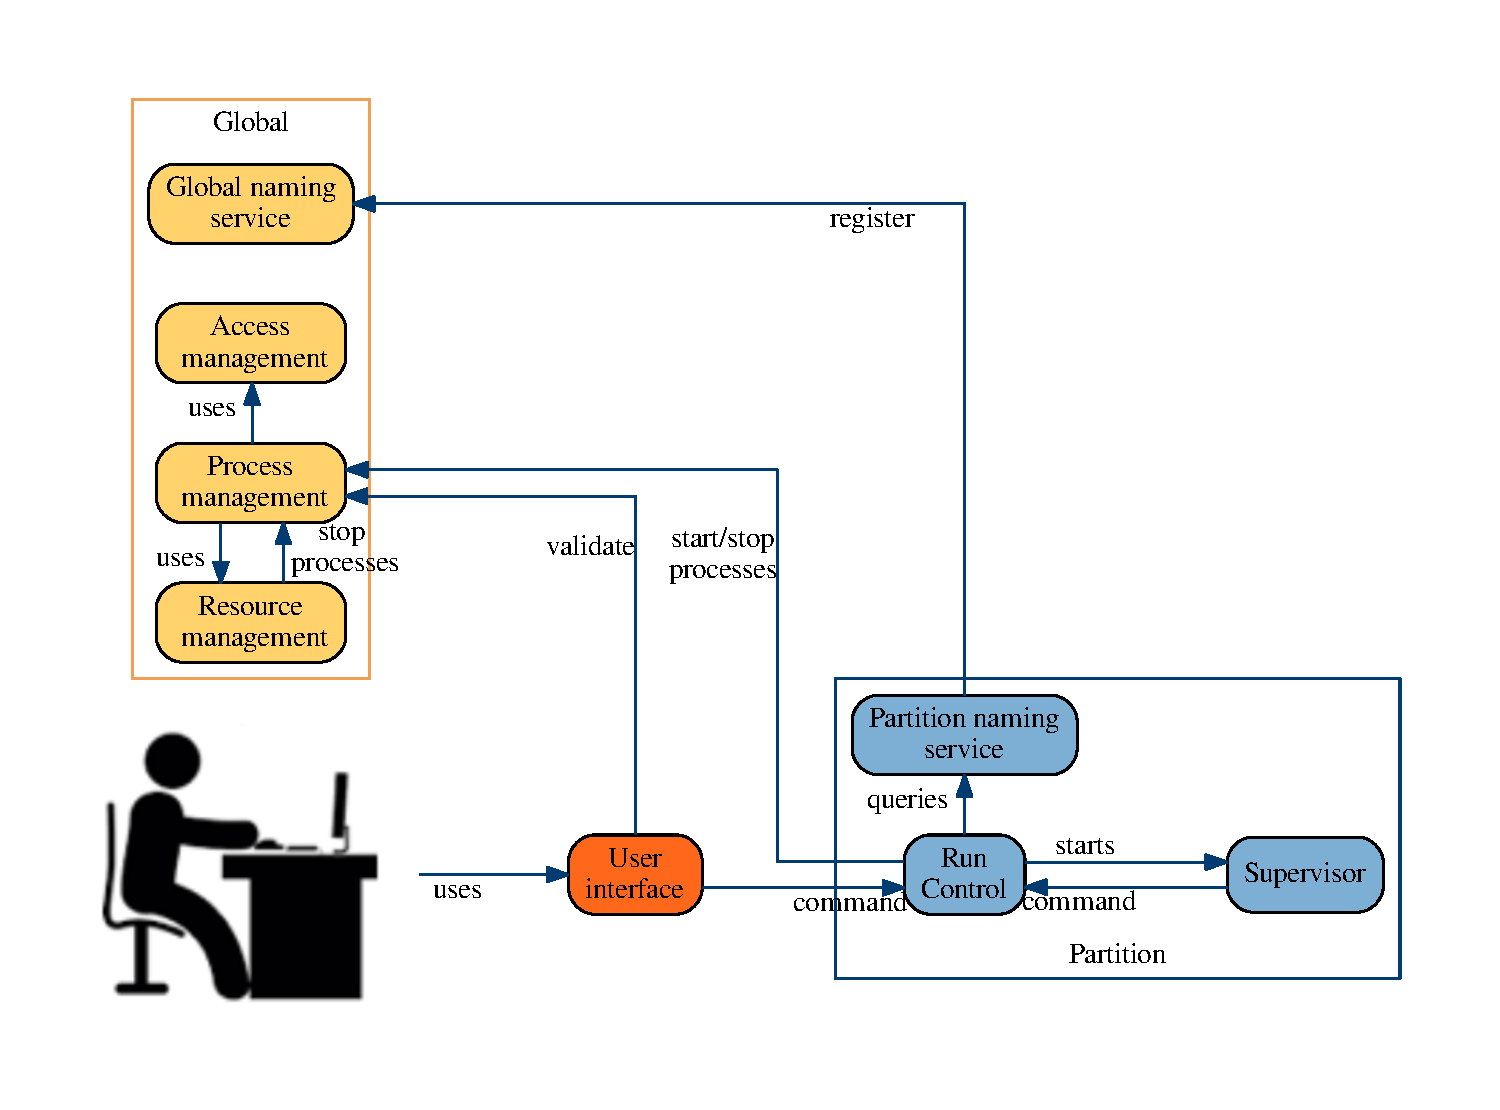
\includegraphics[width=0.8\textwidth]{daq-ccm-control.pdf}
\end{dunefigure}

The control subsystem comprises a number of functional blocks of either global
or partition scope as illustrated in Figure~\ref{fig:daq-ccm-control}. 
In the figure, ``partition'' refers to a logical segmentation of the \dword{daq}
where each segment operates to some extent independently from others. 
The segmentation applies to the portion of detector electronics that provides
input to the partition's \dword{daqdsn} and readout. 
The largest partition %would be
is that of one \dword{detmodule}. 
The functional blocks in the figure represent one or more semi-autonomous
agents, each with defined roles, capabilities, and access. 
Although drawn as single blocks, they typically are implemented as multiple peer
agents to assure redundancy and fail-over. 
The blocks at partition scope are first described.

\begin{itemize}
\item Partition naming service provides \dword{daqdispre} for the components of
  a \dword{daqpart}. 
  That is, it allows one component to be made aware of the creation and
  continued operation of other components (discovery) or that others have
  recently become unresponsive (presence). 

\item Run control provides a central director; its creation is the first step in
  initiating a \dword{daqpart}. 
  The \dword{rc} accepts, interprets, and validates input commands that may come
  either from a human via a user interface, or from other blocks (expert
  systems). 
  The commands describe a desired state of the \dword{daqpart}. 
  \dword{rc} will query other blocks to validate commands and then execute the
  commands by allocating processes through process management. 
  Once successfully allocated, their lifetimes are managed by \dword{rc}. 
  Throughout its lifetime, \dword{rc} will reconfigure an existing process,
  destroy it, or allocate additional processes. 

\item Supervisor provides a locus of expert system automation. 
  This block is instantiated by the \dword{rc} in order to augment or facilitate
  human commands with automated ones. 
  For example, it is expected that some set of commonly occurring exceptions or
  errors will be cataloged as the operators gain experience with the DAQ. 
  Where possible, appropriate responses to these will be codified in the form of
  \dword{rc} commands. 
  The supervisor then will be charged with issuing these commands when one of
  the known exceptions are raised.

\end{itemize}

Global scope controls \dword{daq} components for all \dwords{daqpart} across all
\dwords{detmodule}. 
It consists of the following blocks:


\begin{itemize}
\item Global naming service aggregates the \dword{daqdispre} information across
  partitions.  

\item Process management allocates and may reclaim sets of processes on behalf
  of a requesting component (specifically \dword{rc} and resource management). 
  Process management only allocates processes if their requester has appropriate
  access privileges as determined by access management and if resource
  management determines sufficient resources exist. 
  
\item Resource management determines whether any process allocation can proceed.
  It also enacts process garbage collection to reap any processes which have
  outlived a controlled shutdown command.

\item Access management is responsible for providing authentication and
  authorization for all \dword{daq} functions which require some level of access
  control. 

\end{itemize}

The last block in Figure~\ref{fig:daq-ccm-control} represents a number of
different applications which provide a Human-Machine Interface (UI) to the
control subsystem.
At least one UI will be developed to allow a trained operator to construct and
issue commands required to initiate, configure, potentially reconfigure, and
finally terminate \dwords{daqpart}. 
UIs may enact access control in issuing commands but this does not replace
access control inside the RC when accepting commands.
Any UI used for nominal operation or monitoring of the DUNE FD DAQ (``shift
work'') will be usable remotely from any DUNE institution and from a variety of
personal computing platforms.  
Additional UI elements will be developed as described in
sections~\ref{sec:daq:design:ccm:configuration}
and~\ref{sec:daq:design:ccm:monitoring}.


\subsubsection{Configuration}
\label{sec:daq:design:ccm:configuration}

The \dword{daq} configuration subsystem provides persistent data storage for all
historic, current, and future configuration information applicable to the
\dword{daq}.
It provides a singular point (via high-availability, redundant services) for the
allocation of unique and monotonically increasing \dwords{daqrunnum}.
The configuration data stores operate in an ``insert-only'' mode so that no
prior information may be overwritten. 
The following types of information will be managed:

\begin{itemize}

\item Partition structure contains descriptions of the multiplicity and
  connectivity of \dword{daq} components for any partition. 
  Eg, this describes the overall connectivity of ``nodes'' in the DAQ ``graph''.

\item Component parameters comprise configuration information associated with
  any given \dword{daq} component. 
  Eg, thresholds in a trigger candidate processor or gains and peaking times of
  a FE amplifier.

\item Run number provides a monotonically increasing sequence of
  \dwords{daqrunnum} that are allocated upon request to assure that each is
  unique.

\item Partition instances associate a \dword{daqrunnum} and the set of component
  parameters that were used to initiate a \dword{daqpart} or which are used to
  reconfigure an existing \dword{daqpart}.  

\item Constraints define rules that must be held true by resource management
  servicing requests for process allocations. 
  This information store also includes which constraints were used by resource
  management over time.
\end{itemize}


Access to configuration information is via a service that hides the choice of
storage technology from any client queries.
This interface will also be used by editors run by human operators or by
generators run as part of an expert system.

\subsubsection{Monitoring}
\label{sec:daq:design:ccm:monitoring}

The \dword{daq} monitoring subsystem will help both humans and expert systems in
detecting, diagnosing, and correcting anomalous activity, observing intended
operation, and providing a historical record.
This subsystem will accept required information produced by any \dword{daq}
component (here called status).

The precise implementation of the production, acceptance, store,
post-processing, querying, and visualization of monitored status requires
additional work. 
However, a publish-subscribe (PUB/SUB) network communication pattern is expected
to be adopted for transport of monitoring messages. 
This will decouple production and consumption and facilitate development of a
variety of status viewers, expert systems, debugging tools, etc. 
The types of messages include but are not limited to the following:

\begin{itemize}
\item Common to all will be a ``header'' holding a message type indicator, a
  sender address and the associated detector data time and the recent host
  computer time.
 
\item Logging messages add an importance label (e.g., debug, info, warning,
  error) and a succinct, human-readable information string providing an
  explanation of what occurred.
  
\item Metrics will provide structured data carrying specific information about
  predefined aspects of the sender. 
  This is similar to logging, but the messages support automated consumption and
  reaction by expert systems.  

\item Quality messages summarize information derived from the detector data
  (e.g., from waveforms) or its metadata (e.g., timestamps, error codes) while
  that data is ``in flight'' through the \dword{daq}.

\end{itemize}

In general, the DAQ will retain all status records at least long enough to allow
for any offline data quality validation procedures to be performed. 
However, some status feeds may be processed prior to storage if their raw form
requires prohibitive amount of storage. 
In particular, the quality stream data rate may be too substantial for long term
storage. 
Such streams will be summarized into histograms or other statistical
representations prior to storing for longer term use.

In addition to this \dword{daq} \dword{daqccm} monitoring subsystem, a separate
system must be used to monitor in depth the quality of the detector data content
itself. 
See Section~\ref{sec:daq:design-data-quality} for the description of this data
quality monitoring system.

\subsection{Inter-Process Communication}
\label{sec:daq:design-ipc}

The DUNE FD DAQ is an asynchronous, parallel distributed data processing system. 
It is composed of many independent processes which ingest and produce messages. 
The mechanisms of such message passing are generally called \dword{ipc}. 
Referring to Figure~\ref{fig:daq:layout}, IPC is used for both in-band detector
data flow between Upstream DAQ and back-end Event Builders and for out-of-band
messages as part of Control, Configuration and Monitoring. 
The IPC used by the Data Selection spans both descriptions as it passes
derivations of a subset of detector data (trigger primitives, candidates) and
culminates in a source of out-of-band message (trigger commands) to direct the
readout by Event Builder and other components of detector data that is held in
the Upstream DAQ buffers.

The ZeroMQ~\cite{zeromq} smart socket library is the basis of a system being
developed and evaluated for parts of both in-band and out-of-band IPC. 
As part of the CCM, this include the issuing of control and reconfiguration
commands to and receiving of monitoring messages from essentially all DAQ
components. 
As part of Data Selection, this includes the transfer of trigger primitive,
candidate and command messages. 
In the Upstream DAQ this includes the Buffer Interface Service which provides
access to the Upstream DAQ primary buffers for queries by Event Builder and
other components. 
IPC must be implemented broadly across many DAQ systems and ZeroMQ allows their
problems to be solved in common, shared software. 
As CCM has the most complex IPC needs, this work is organizationally considered
part of this system.

One ZeroMQ facility in particular is worth additional description. 
Zyre will provide a decentralized implementation \dword{daqdispre} (see
Section~\ref{sec:daq:design:ccm:control}). 
It uses UDP broadcast beacons and a connected followup to provide peer discovery
on the local network. 
A heartbeat mechanism provides presence so that a compent may discover when a
peer has become unresponsive.  
As Zyre uses the network itself, there is no central point of failure. 
The network provides the naming service described above. 
Zyre also allows for more centralized, connection oriented, discovery which can
be used to allow the process to span networks.

As described in~\ref{sec:daq:design-backend}, \textit{artDAQ}~\cite{artdaq}
utilizes IPC between its back-end components. 
It has been well tested with ProtoDUNE and other experiments. 
ArtDAQ may be used for some portions of the IPC described above. 
For example, if the Buffer Interface Service is implemented as an artDAQ Board
Reader it would necessarily use artDAQ IPC. 
This would limit the types of clients that could query for data in the buffers
to be artDAQ modules. 
Understanding how to optimally select an IPC for such parts of the DAQ
connection graph is an area of ongoing R\&D effort.

\subsection{Timing and Synchronization}
\label{sec:daq:design-timing}

All components of the \dword{fd} use clocks derived from a single \dfirst{gps}
disciplined source, and all module components are synchronized to a common
\SI{62.5}{MHz} clock. 
To make full use of the information from the \dword{pds}, the common clock must
be aligned within a single detector module with an accuracy of
\bigo{\SI{1}{\nano\second}}. 
For a common trigger for a \dword{snb} between modules, the timing must have an
accuracy of \bigo{\SI{1}{\milli\second}}.
However, a tighter constraint is the need to calibrate the common clock to
universal time derived from \dword{gps} so the \dword{daqdsn} algorithm can be
adjusted inside an accelerator spill, which again requires an absolute accuracy
of \bigo{\SI{1}{\micro\second}}.

The \dword{dune} \dword{fd} uses a version of the \dword{protodune} timing
system, where a design principle is to transmit synchronization messages over a
serial data stream with the clock embedded in the data. The format is described
in \citedocdb{1651}. The timing system design is described in detail in
\citedocdb{11233}.

Central to the timing system are four types of signals:
\begin{itemize}
\item a \SI{10}{\mega\hertz} reference used to discipline a stable master clock,
\item a \dfirst{pps} from the GPS,
\item a \dword{ntp} signal providing an absolute time for each \dword{pps}, and
\item an \dfirst{irig} time code signal
  used to set the timing system 64-bit time stamp.
\end{itemize}

The timing system synchronization codes are distributed to the \dword{daq}
readout components in the \dfirst{cuc} and the readout components on the
cryostat via single mode fibers and passive splitters/combiners.
All custom electronic components of the timing system are contained in two
\dword{utca} shelves; at any time, one is active while the other serves as a hot
spare.
The \SI{10}{MHz} reference clock and the \dword{pps} signal are received through
a single-width \dword{amc} at the center of the \dword{utca} shelf.
This master timing \dword{amc} is a custom board and produces the timing system
signals, encoding them onto a serial data stream.
This serial data stream is distributed over a backplane to a number of fanout
\dwords{amc}.
The fanout \dword{amc} is an off-the-self board with two custom \dwords{fmc}.
Each \dword{fmc} has four \dword{sfp} cages where fibers connect the timing
system to each detector component or where direct attach
cables connect to other systems in the \dword{cuc}.

To provide redundancy, two independent GPS systems are used, one with an antenna
at the surface of the Ross shaft, and the other with an antenna at the surface
of the Yates shaft.
Signals from either GPS are fed through optical single mode fibers to the
\dword{cuc}, where either GPS signal can act as a hot spare while the other is
active. 
Differential delays between these two paths are resolved by a second pair of
fibers, one running back from the timing system to each antenna.
The GPS receiver at the  \dword{cuc} generated the 1PPS and 10MHz analog signals which are used to feed
the White Rabbit Grand Master switch of the DP electronics timing system.
%\fixme{Need we say something about the how the DAQ timing system connects to the DP electronics timing system?}


\section{Design Validation and Development Plans}
\label{sec:daq:validation}

\fixme{This section still needs a lot of work to add DP-specific validation.}

This section starts with a description of the generic DAQ validation
efforts and ends with those specific to interfacing the DAQ with DP
electronics. 
As described above, the majority of design elements of the DUNE FD DAQ
are intentionally independent from details of the detector, its
electronics and the form and content of the data they provide as input
to the DAQ. 
The differences are accommodated by the thin, custom hardware boundary
layer composed of FELIX boards. 
This boundary provides the first and primary translation or ``type
erasure'' so that more generic data forms may then by processed by the
DAQ internals.
As it happens, the \dword{pdsp} experiment has been used as a vehicle to
validate many solutions to challenges common to servicing both DP and SP
detector technology.

While FELIX absorbs technical differences in formats, rates, etc, some
validations described below are sensitive to the information content of
their input data. 
Specifically, the fraction, form and type of the data that is input to
self-triggering studies determines to some extent the performance of the
DAQ element being validated.
It can be argued in many cases that a successful validation performed
with SP data ensures a successful outcome with equivalent DP data.
The reasons for this become obvious given the following facts which
compare DP \dword{cro} data to SP TPC equivalents:
\begin{itemize}
\item larger signal-to-noise ratio allows thresholds used in
  self-triggering to be more effective.
\item all channels provide unipolar ``collection'' waveforms which may
  be compared immediately and without costly deconvolution to noise
  levels (although, it must be said that both DP and SP cover their
  entire sensitive area with ``collection'' electrodes).
\item the sensitive electrodes are grouped as to provide localized 2D
  segmentation which is at least as effective for self-triggering as
  that which is provided by SP ``collection wires''.
\end{itemize}


Given this practical adaptation of SP data in the validation of DAQ
elements for servicing DP detector technology, the following strategy
governs the general validation and development of the \dword{dune}
\dword{fd} \dword{daq} design:
\begin{itemize}
\item Use of \dword{protodune} as a design demonstration and
  development platform. 
\item Use of vertical slice teststands for further development and testing of
  individual \dword{daq} subsystems and for key aspects of the
  overall \dword{daq}
\item Use of horizontal slice tests to demonstrate scaling the design
  where the multiplicity of components in subsystem layers is important.
\item Use of \dword{fd} MonteCarlo simulations and emulations in order
  to augment actual hardware demonstrations at \dword{protodune} and teststands.
\item Benefit from developments and measurements from other ongoing
  LArTPC experiments, including MicroBooNE, SBND, and ICARUS.
\end{itemize}

This strategy reflects the current \dword{daq} project schedule,
provided in Section~\ref{sec:daq:schedule}, which
comprises several phases, including an intense development phase
through 2020 that culminates in an engineering design
review (EDR) in Q1 of 2021. At this milestone, the system design will be
finalized and demonstrated to be capable of meeting the requirements of the
final \dword{daq} system. After the development phase, a
pre-production phase will begin and will end with a production readiness
review (PRR). By then, final designs of all components
will be complete.

The following subsections summarize past, ongoing, and planned
development and validation studies and identify how anticipated outcomes
will be used to finalize the \dword{daq} design.

\subsection{Design Validation and Development at ProtoDUNE and Other
  LArTPC Experiments}


\label{sec:daq:protodune}

The \dword{fd} \dword{daq} consortium constructed and operated a
\dword{daq} system for \dword{protodune} based on \dword{felix},
develped by ATLAS~\cite{pdsp-felix} which largely represents the general
design for DUNE FD DAQ.
\dword{daq} design and construction for \dword{protodune} began in Q3 of
2016, and the system became operational at the start of the beam data
run in Q4 of 2018.
The detector is continuing to run as of the writing of this document,
recording cosmic ray activity, and providing further input for
\dword{daq} development toward \dword{dune}. 

Besides the differences in horizontal scale between \dword{protodune}
and \dword{dune} FD, their \dwords{daq} exhibit these key differences. 
\begin{itemize}
\item The \dword{protodune} \dword{daq} is externally triggered while
  DUNE FD must be. 
\item The \dword{protodune} detectors are on the surface of the Earth
  with minimal overburden. 
  Regardless of trigger mechanism, every readout contains substantially
  more signal activity than expected from an ``average'' readout of DUNE
  FD.
\item The trigger rate of \dword{protodune} detectors is more than two
  orders of magnitude larger than expected at DUNE FD.

\end{itemize}

The first difference illustrates that the production \dword{protodune}
DAQ does not test self-triggering thus validating this ability is of a
prime intereste.
As described in Section~\ref{sec:daq:design-data-selection}, it is the
\dword{daqdsn} which provides self triggering and is a central component
in validation and development plans.
 
On the other hand, the latter two items illustrate that
\dword{protodune} DAQ has in some ways solved harder challenges (at its
given horizontal scale) than will be seen in the DUNE FD. 
The instantaneous rate, per unit of detector is far higher in
\dword{protodune} than DUNE FD. 
The information (signal) content of the data is also higher. 
Thus, local validations on \dword{protodune} assures good performance at
DUNE FD. 
What remains is the relatively ``mechanical'' demonstration that the
required horizontal scaling can be achieved.  

\subsection{ProtoDUNE Outcomes}

Despite being designed for a much more limited horizontal scale than
DUNE, the successful operation of the \dword{protodune} \dword{daq} has
provided several key demonstrations for \dword{dune} FD \dword{daq}, in
particular data flow architecture, run configuration and control, and
back-end functionality.
More specifically, \dword{protodune} has demonstrated

\begin{itemize}
\item Front-end Readout: successful front-end readout hardware and data
  flow functionality for the readout of two out of the six APAs employed
  in protoDUNE.
  This was achieved with two TPC RU's, without co-processor boards, and
  only one APA read out per FELIX board.
  The \dword{dune} DAQ design will ultimately accommodate readout of two
  APAs per FELIX board.
  This readout poses a higher per-fiber data throughput challenge than
  needed for reading out DP crates. 
  However, this tests a synchronous, uncompressed data stream. 
  Testing the receiving of compressed data over UDP from DP crates by
  FELIX will be demonstrated in future validations.

  In addition to data flow functionality, ProtoDUNE Front-end readout
  has been demonstrated to interface to (SP) front-end electronics for
  the purpose of control and configuration. 
  Future validation effort will evaluate what elements need to be
  developed to likewise interface with DP electronics in an equivalent
  manner.

\item Back-end DAQ and Software Infrastructure: successful back-end
  DAQ implementation, including event builder farm and disk buffering.
  This has allowed the development and exercising of system
  partitioning, and provides a basis for scalability to DUNE.
  ProtoDUNE also serves as a platform for further system development

\item Data Selection and Timing: successful operation of the timing
  distribution system, and external trigger distribution to the
  front-end readout.
  Although protoDUNE was externally triggered, the system serves as a
  development platform for data-driven data selection.
\end{itemize}

Besides demonstrating end-to-end data flow, an important outcome of
\dword{protodune} DAQ has been the delineation of interfaces, i.e.~understanding
the exact \dword{daq} scope and the interfaces to TPC, \dword{pds}, and
offline.
The use of commercial off-the-shelf solutions where possible, and
leverage of professional support from CERN IT substantially expedited
the development and success of the project, as did the strong on-site
presence of experts from within the consortium during early installation
and commissioning. 

Outcomes specific to \dword{protodune} subsystems are discussed in
greater detail
in~\cite{talkfromCDR}. Figure~\ref{fig:sp-daq:protodunedaqpic} shows the
ProtoDUNE DAQ hardware as used during beam data taking.

\begin{dunefigure}{fig:daq-rates}{ProtoDUNE DAQ hardware as used during beam data taking. \label{fig:sp-daq:protodunedaqpic}}
  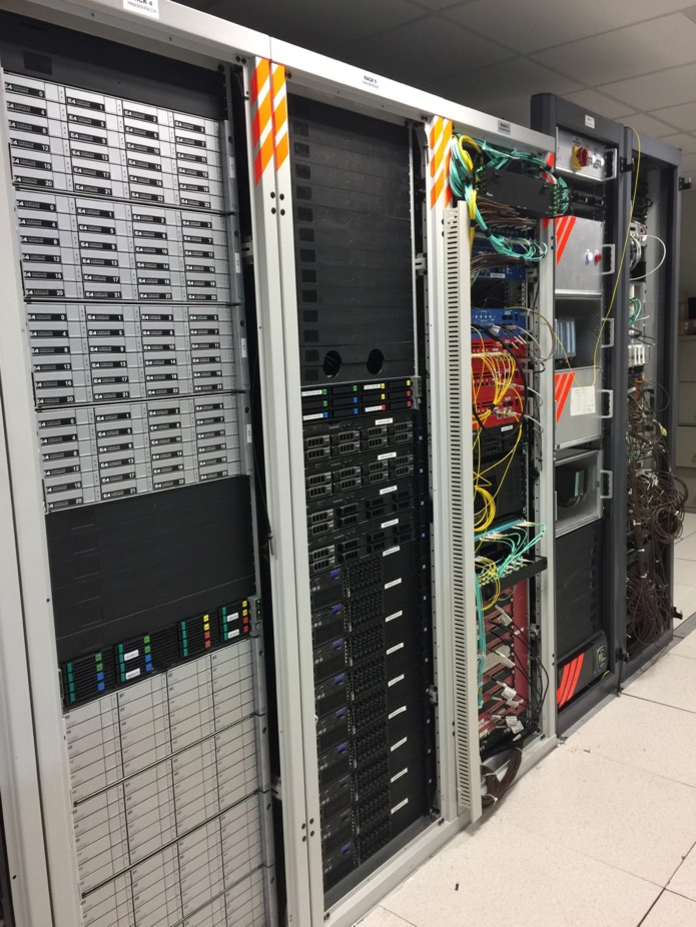
\includegraphics[height=0.5\textheight]{DAQ_hardware_NP04.pdf}
\end{dunefigure}


\subsection{Ongoing Development}
\label{sec:daq:design-validation}


Subsystem development is ongoing at ProtoDUNE at the time of the
writing of this document. A detailed schedule for 2019 is available
in \cite{referencedocdbfromgiovanna}. Major development plan milestones are:
\begin{itemize}
\item optimization and tuning of the Front-end readout
\item optimization and tuning of the artdaq based dataflow software
\item enhancement of monitoring and troubleshooting capabilities
\item introduction of basic self-triggering support mechanism
\item implementation self-triggering algorithms which are sensitive to
  particular signal activity 
\item prototyping of data flow patterns in front-end and back-end
  relevant to SNB triggering.
\end{itemize}

Below, we focus on ongoing developments related to upstream DAQ,
data selection, which is a key challenge for DUNE and new with respect
to ProtoDUNE (and other existing or planned LArTPC detectors),
and IPC, which is common across multiple DAQ subsystems.


\subsubsection{Upstream DAQ Development}

The use of FELIX as the front-end readout technology for DUNE was successfully
prototyped at ProtoDUNE, initially for the readout of one SP APA.
In ProtoDUNE, FELIX allows streaming of data coming over multiple 10 Gbps
optical point-to-point links into commercial host memory and, from there,
storing, dispatching or processing of the data via software. 


\begin{dunefigure}{fig:sp-daq:felix-pd-impl}{The topology of the FELIX based
    upstream DAQ of ProtoDUNE (from~\cite{pdsp-felix}). The FELIX host servers are publishing the data from the WIBs over 100Gb network interfaces. The BoardReader hosts are carrying out trigger matching, data compression and forwarding of fragments to the event builder.}
  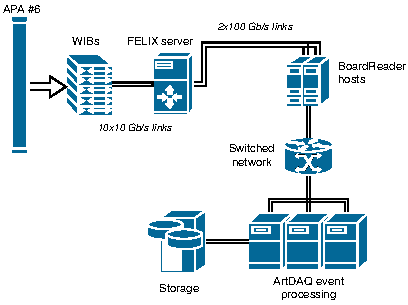
\includegraphics[width=0.7\textwidth]{daq-pdsp-felix-system.pdf}
\end{dunefigure}

The test utilized three host computers as illustrated in
Figure~\ref{fig:sp-daq:felix-pd-impl}.
One hosting the FELIX board is connected to two hosting software
applications over a 100 Gbps network.
The FELIX I/O card interfaces with its host through 16-lane PCIe Gen3.
This interfaces sees a bit less than half of the theoretical max
bandwidth of \SI{16}{GB/s}.
Over this, FELIX transfers its input data into the host PC memory via
continuous DMA transfer.
The FELIX host runs a software process which publishes data over the
network to subscribing clients.
Subscriptions are based on optical link identifiers.
The primary subscribers are \dword{artdaq} BoardReader processes.
In order to sustain the data rate, modest modifications of the firmware
(increased block size and chunk merging) and software (scatter-gather
publisher) were carried out specifically for ProtoDUNE: the FELIX host
receives and publishes data at ~75 Gbps.
The BoardReader hosts are equipped with embedded Intel QuickAssist (QAT)
\cite{qat} technology for hardware accelerated data compression.


Benchmarking and optimization of the FELIX firmware and software will also
continue, with the aim of further concentrating the number of \dwords{cro} and
\dwords{lro} per RU host computer.

\fixme{Give estimate of CRO/LRO per RU.}

\subsubsection{Data Selection Development}

\begin{dunefigure}{fig:daq-cpu-hf-speed}{CPU core-time (left) required
    to find primitives in simulated signal and noise data across 960
    channels.
    In this test the data has been pre-formatted to facilitate the use
    of SIMD hardware accelerated functions (AVX2). 
    CPU utilization in live data (right) for both reformatting and
    trigger primitive generation. 10 CPU at about 65\% utilization are
    required to keep up. 
    The initial peak is due to faster than nominal deliver of input due
    to startup buffering issues. 
    The system is able to catch up with the backlog.
    Importantly, neither of these two tests include the necessary data
    decompression step.}
  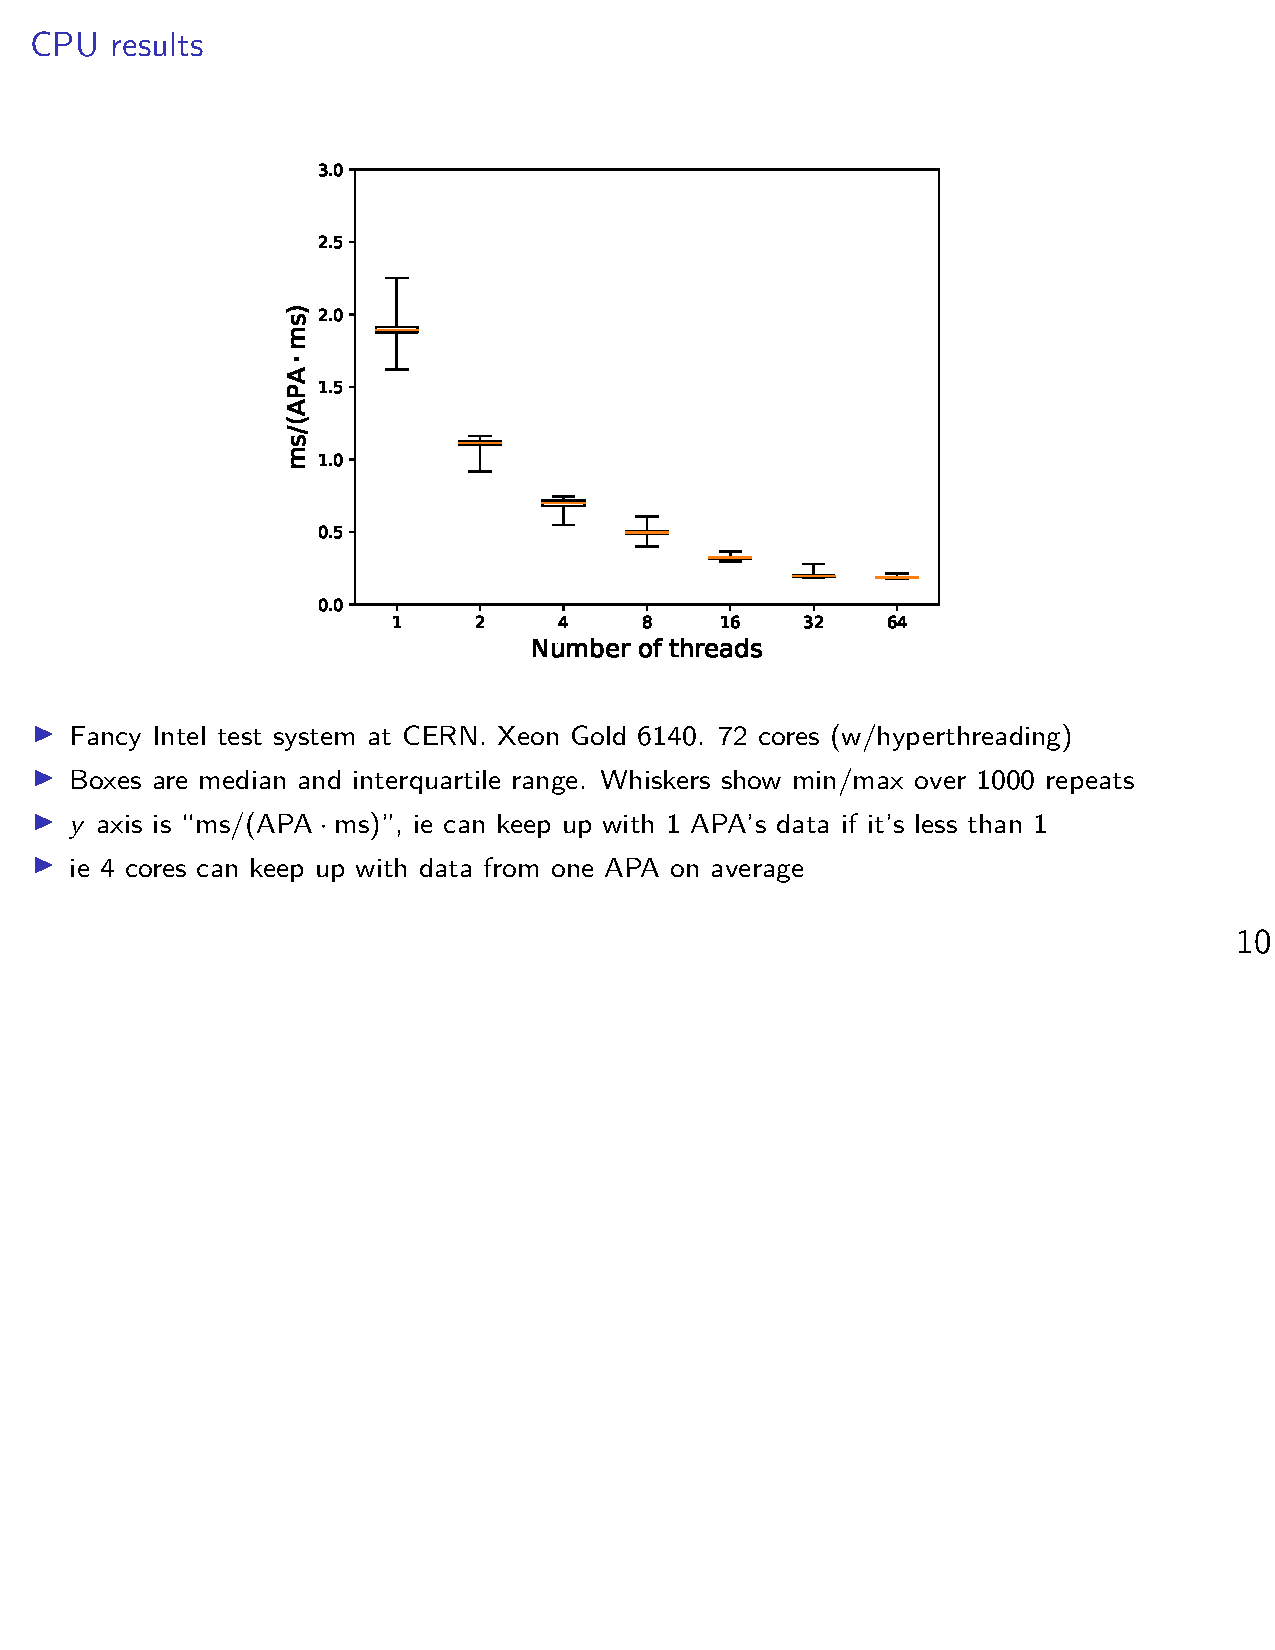
\includegraphics[height=5cm,clip,trim=4cm 16cm 4cm 2cm]{daq-primitive-cpu-speed.pdf}%
  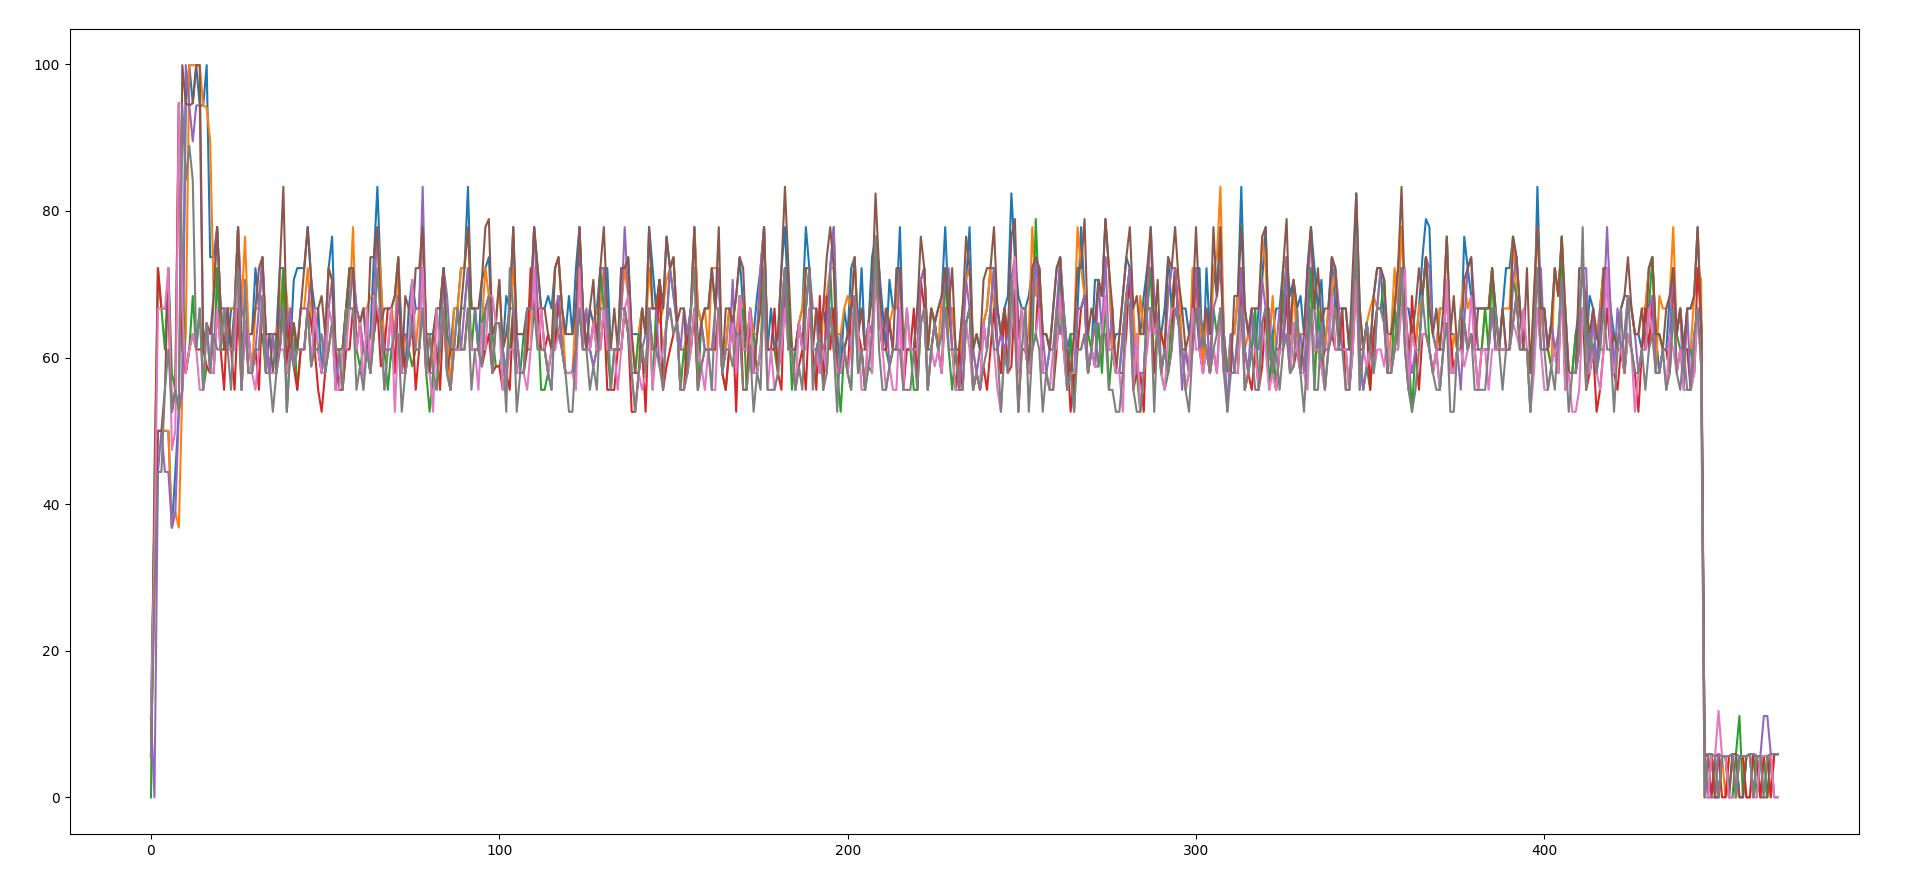
\includegraphics[height=5cm,clip,trim=0cm 0cm 0cm 0cm]{daq-hf-felix-sp-live.png}
\end{dunefigure}

\begin{dunefigure}{fig:daq-hitfinder}{Illustration of the trigger primitives
    found by the CPU algorithm in one nominal readout of one APA face in ProtoDUNE-SP
    data.  Although the data was ultimately recorded due to trigger, the
    algorithm ran in full-stream mode.  Similar algorithms will have an easier
    problem to solve with DP waveforms due to their higher signal/noise ratio
    compared to SP collection channels.}
    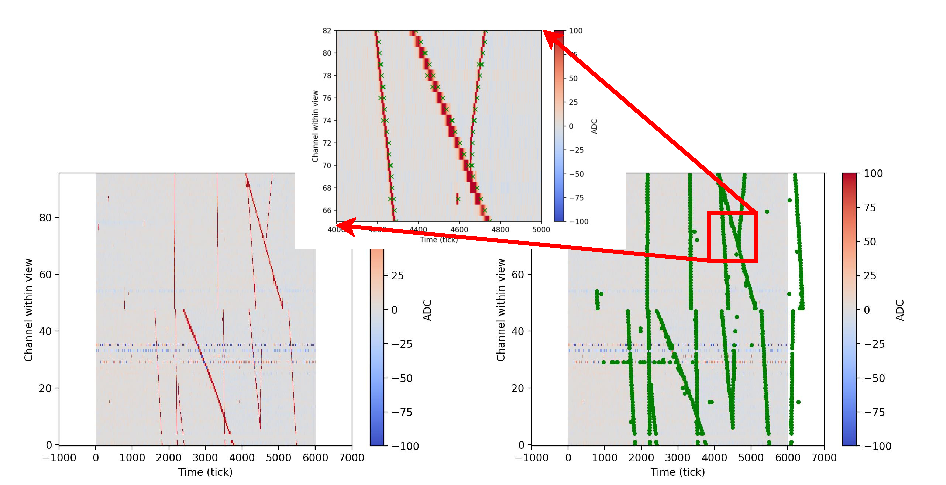
\includegraphics[width=0.9\textwidth]{daq-hitfinder-montage.pdf}
\end{dunefigure}

\begin{dunefigure}{fig:daq-tp-rates}{Trigger primitive rates in ProtoDUNE-SP as
    a function of threshold in four categories: all data (top left), after
    removal of particularly noisy channels (top right), with HV off so no
    contribution to signal (bottom left) and HV off and noisy channels excluded
    (bottom right). \fixme{These tests need to be redone or translated
      into implications for DP data.}}
  \begin{minipage}[b]{0.5\linewidth}
    \begin{center}
      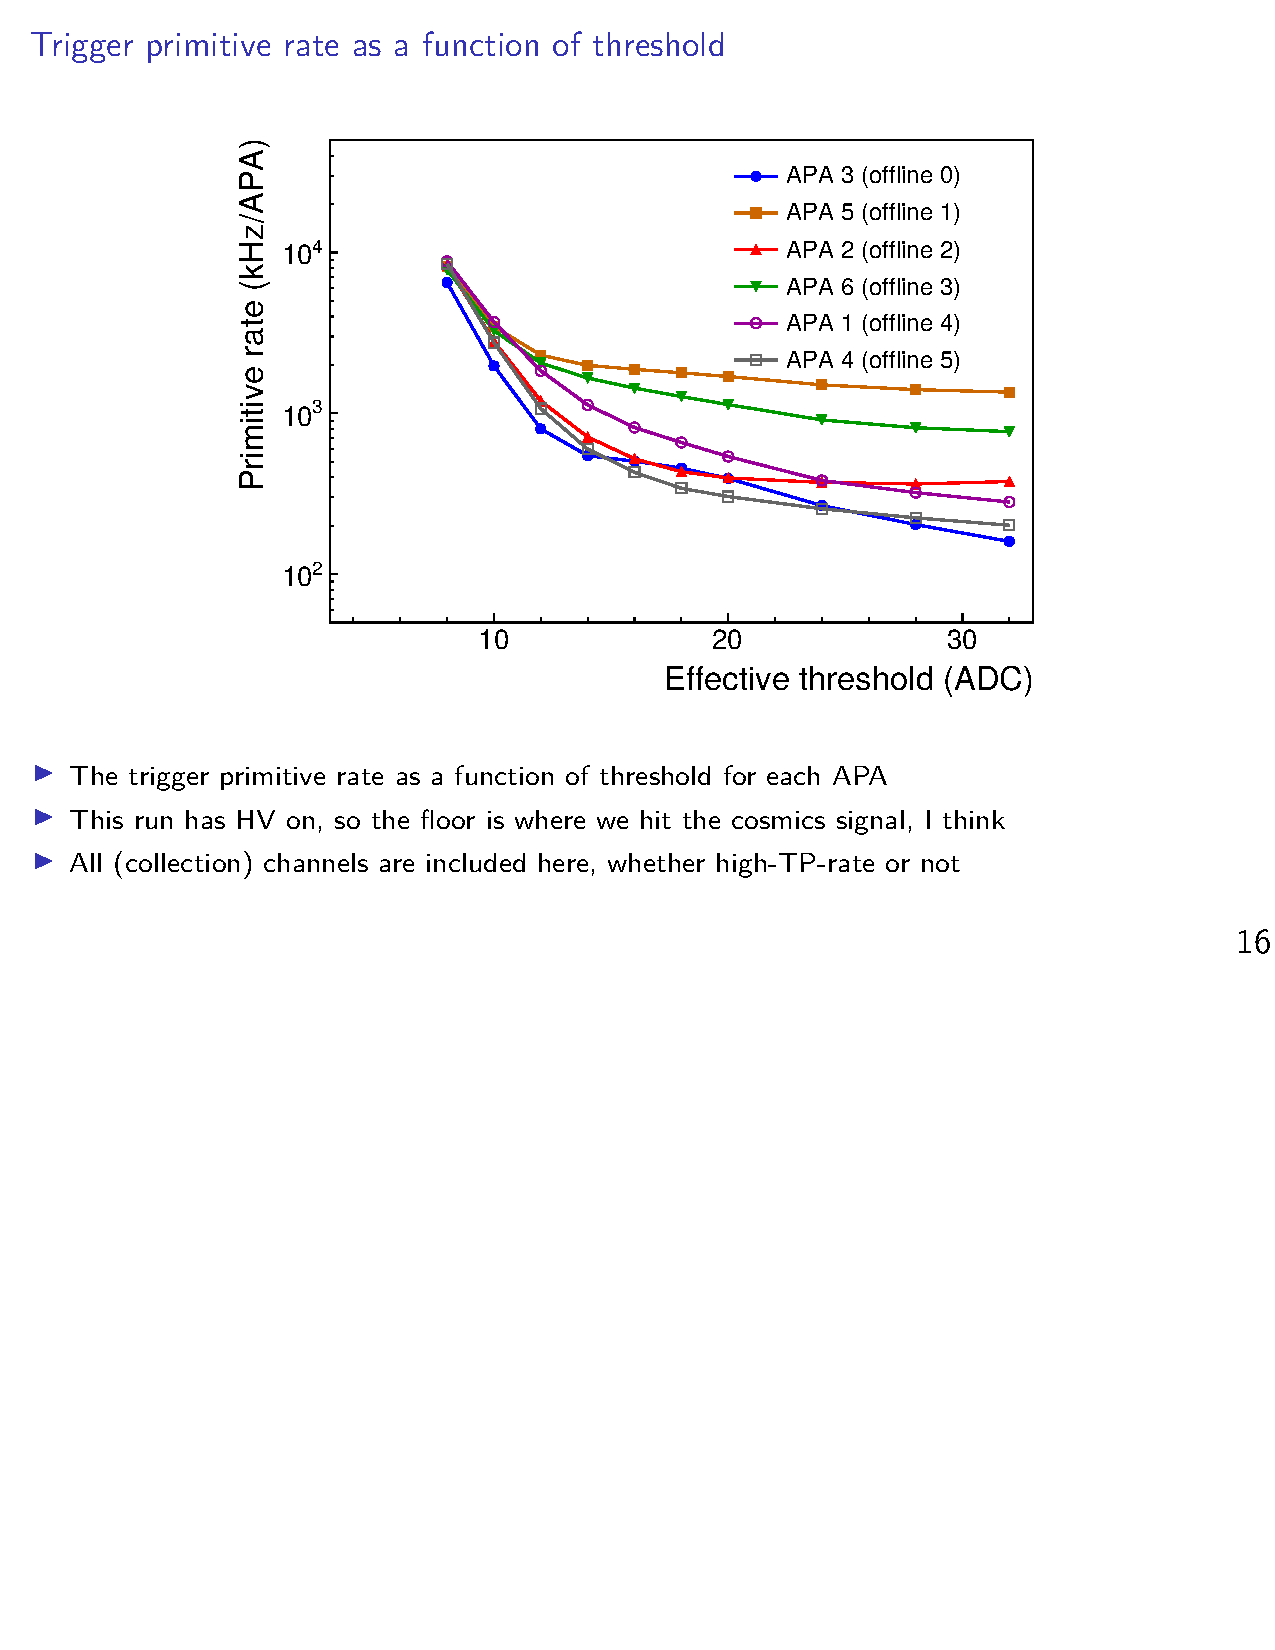
\includegraphics[page=1,width=0.8\textwidth,clip,trim=4cm 16cm 4cm 2cm]{daq-primitive-rates-thresholds.pdf}

      \includegraphics[page=2,width=0.8\textwidth,clip,trim=4cm 16cm 4cm 2cm]{daq-primitive-rates-thresholds.pdf}
    \end{center}
  \end{minipage}%
  \begin{minipage}[b]{0.5\linewidth}
    \begin{center}
      \includegraphics[page=3,width=0.8\textwidth,clip,trim=4cm 16cm 4cm 2cm]{daq-primitive-rates-thresholds.pdf}

      \includegraphics[page=4,width=0.8\textwidth,clip,trim=4cm 16cm 4cm 2cm]{daq-primitive-rates-thresholds.pdf}
    \end{center}
  \end{minipage}

\end{dunefigure}


During early stages of design, significant effort has been dedicated on
trigger primitive generation through simulations.
Specifically, charge collection efficiency and fake rates due to noise
and radiologicals have been studied as a function of hit threshold,
demonstrating that requirements can be met, given sufficiently low
electronics noise levels and radiological rates \cite{ref}.
Ongoing efforts within DUNE's Radiologicals Task force aim to validate
or provide more accurate background predictions, upon which this
performance will be validated.
In addition, offline studies demonstrate the performance of trigger
primitive generation algorithms as a function of number of CPU cores
used.  
The results are summarized in Figure~\ref{fig:daq-cpu-hf-speed} and show
that four cores as sufficient to keep up with 960 channels.
The test does not include reformatting of the data required to put it in
a form that allows hardware SIMD acceleration (AVX).  
In tests with live \dword{protodune} data, it is found that ten cores at
and average 65\% usage were enough to handle both reformatting and
trigger primitive selection. 
Effort on understanding and removing contribution from
cosmics/cosmogenics and (known) noisy channels is ongoing.
These results are summarized in Figure~\ref{fig:daq-tp-rates}

\begin{dunefigure}{fig:daq-tc-eff-vis}{Efficiency for forming trigger
    candidates as input trigger primitives from two algorithms, online
    (blue) and offline (red) applied to \dword{pdsp}. \fixme{These need
      to be redone for DP}}
  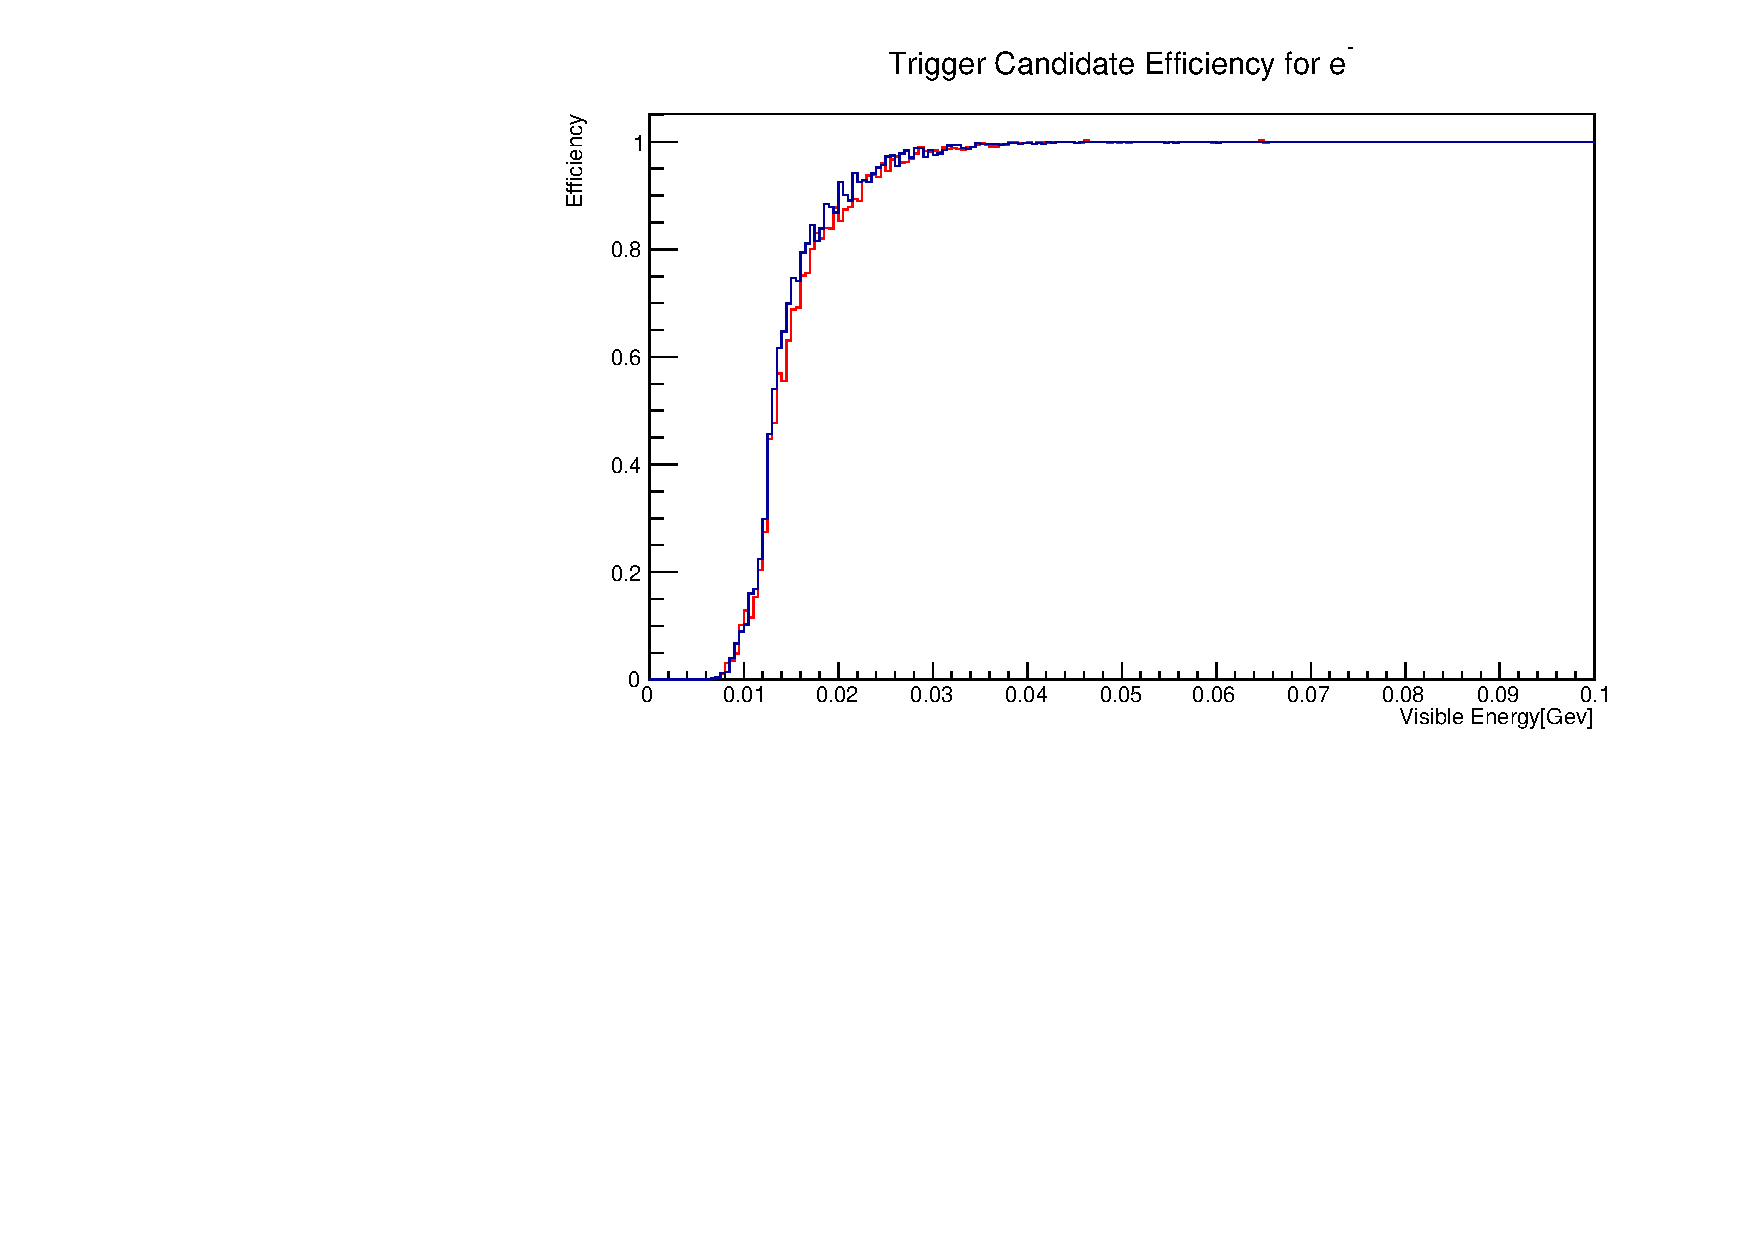
\includegraphics[width=0.7\textwidth]{Electron_Efficiency_Comparison.pdf}
\end{dunefigure}

\begin{dunefigure}{fig:daq-tc-eff-true}{All-inclusive, integrated
    efficiency for forming trigger candidates from ionization activity
    from beam $\nu_e$ (left) and beam $\nu_\mu$ (right) interactions at
    or above a given true neutrino energy. 
    The trigger candidate algorithm used is the offline version, see
    Figure~\ref{fig:daq-tc-eff-vis} for comparison with online version.  \fixme{These need
      to be redone for DP}}
  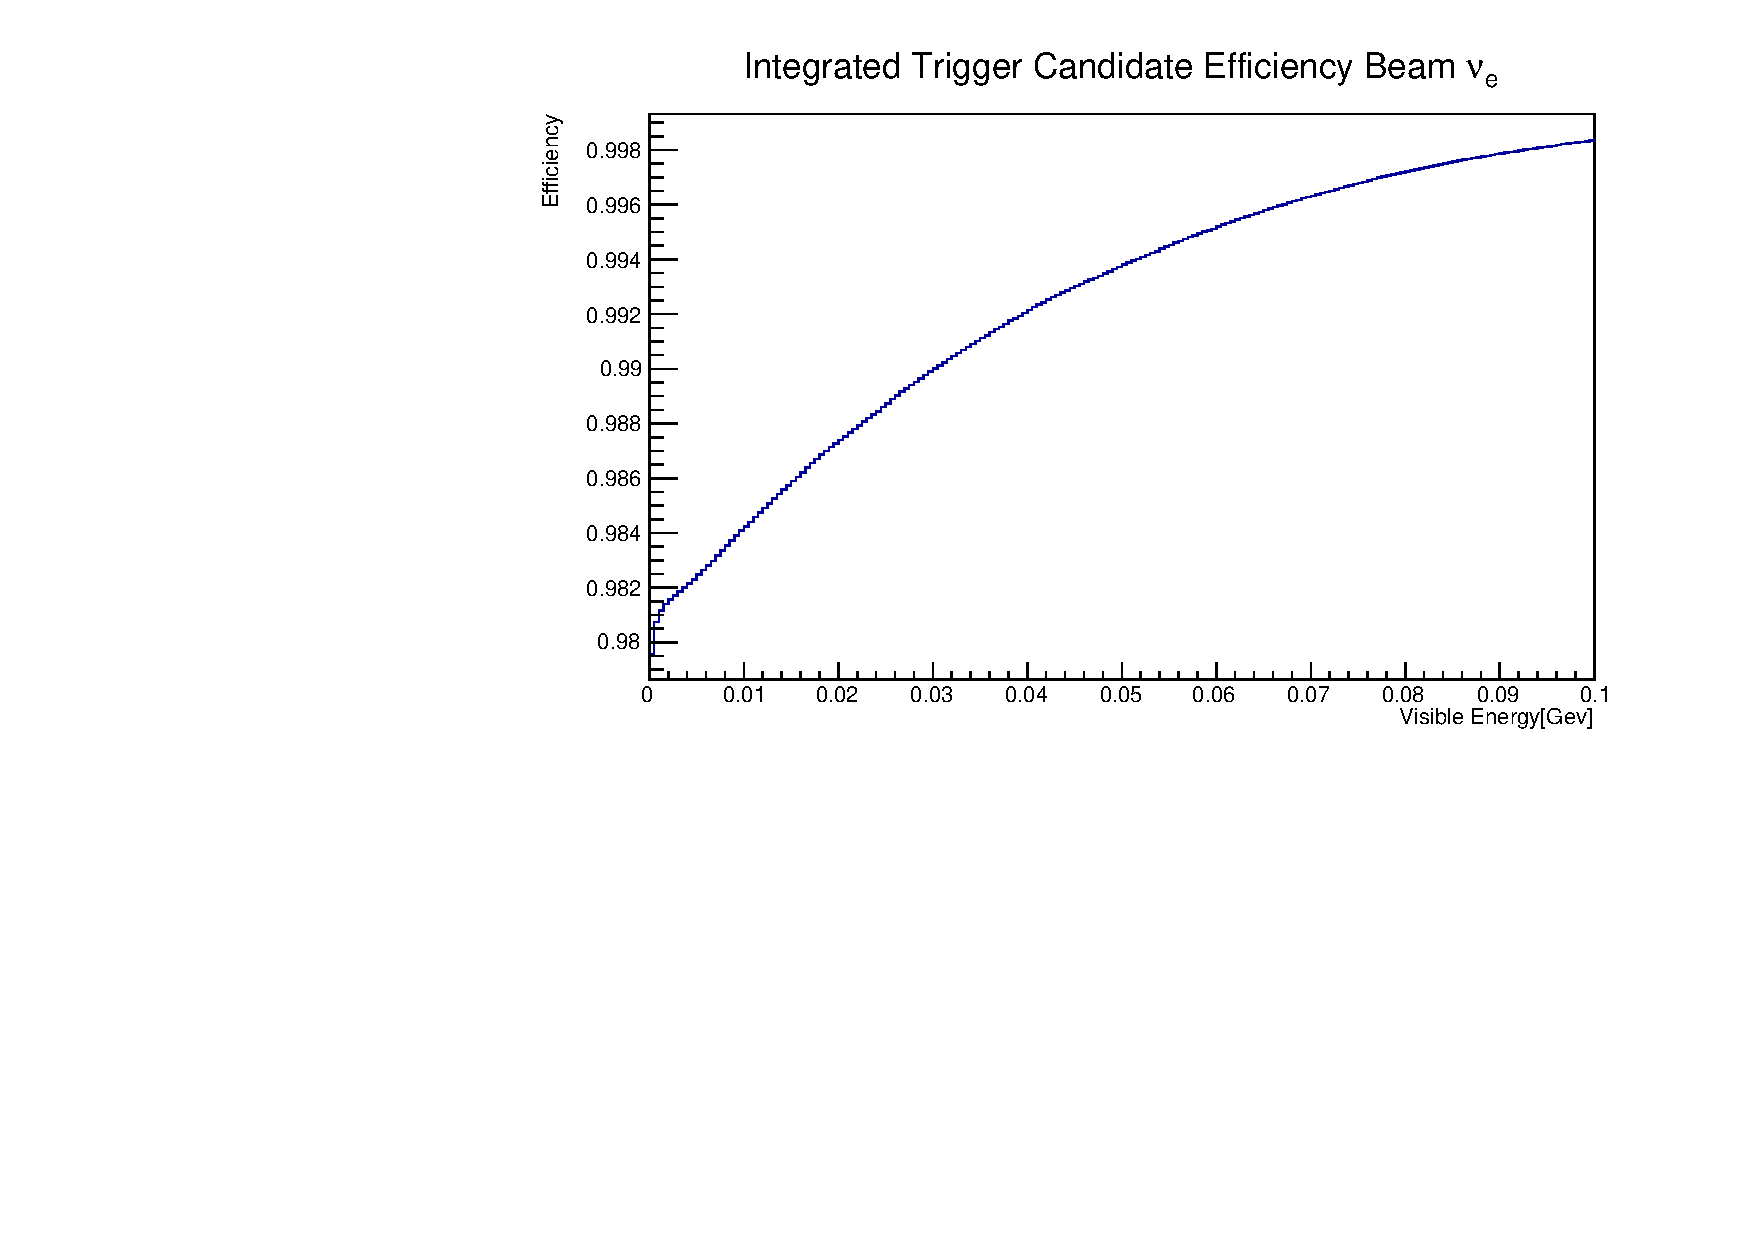
\includegraphics[width=0.45\textwidth]{Integrated_Nu_e_Efficiency_MCC10.pdf}%
  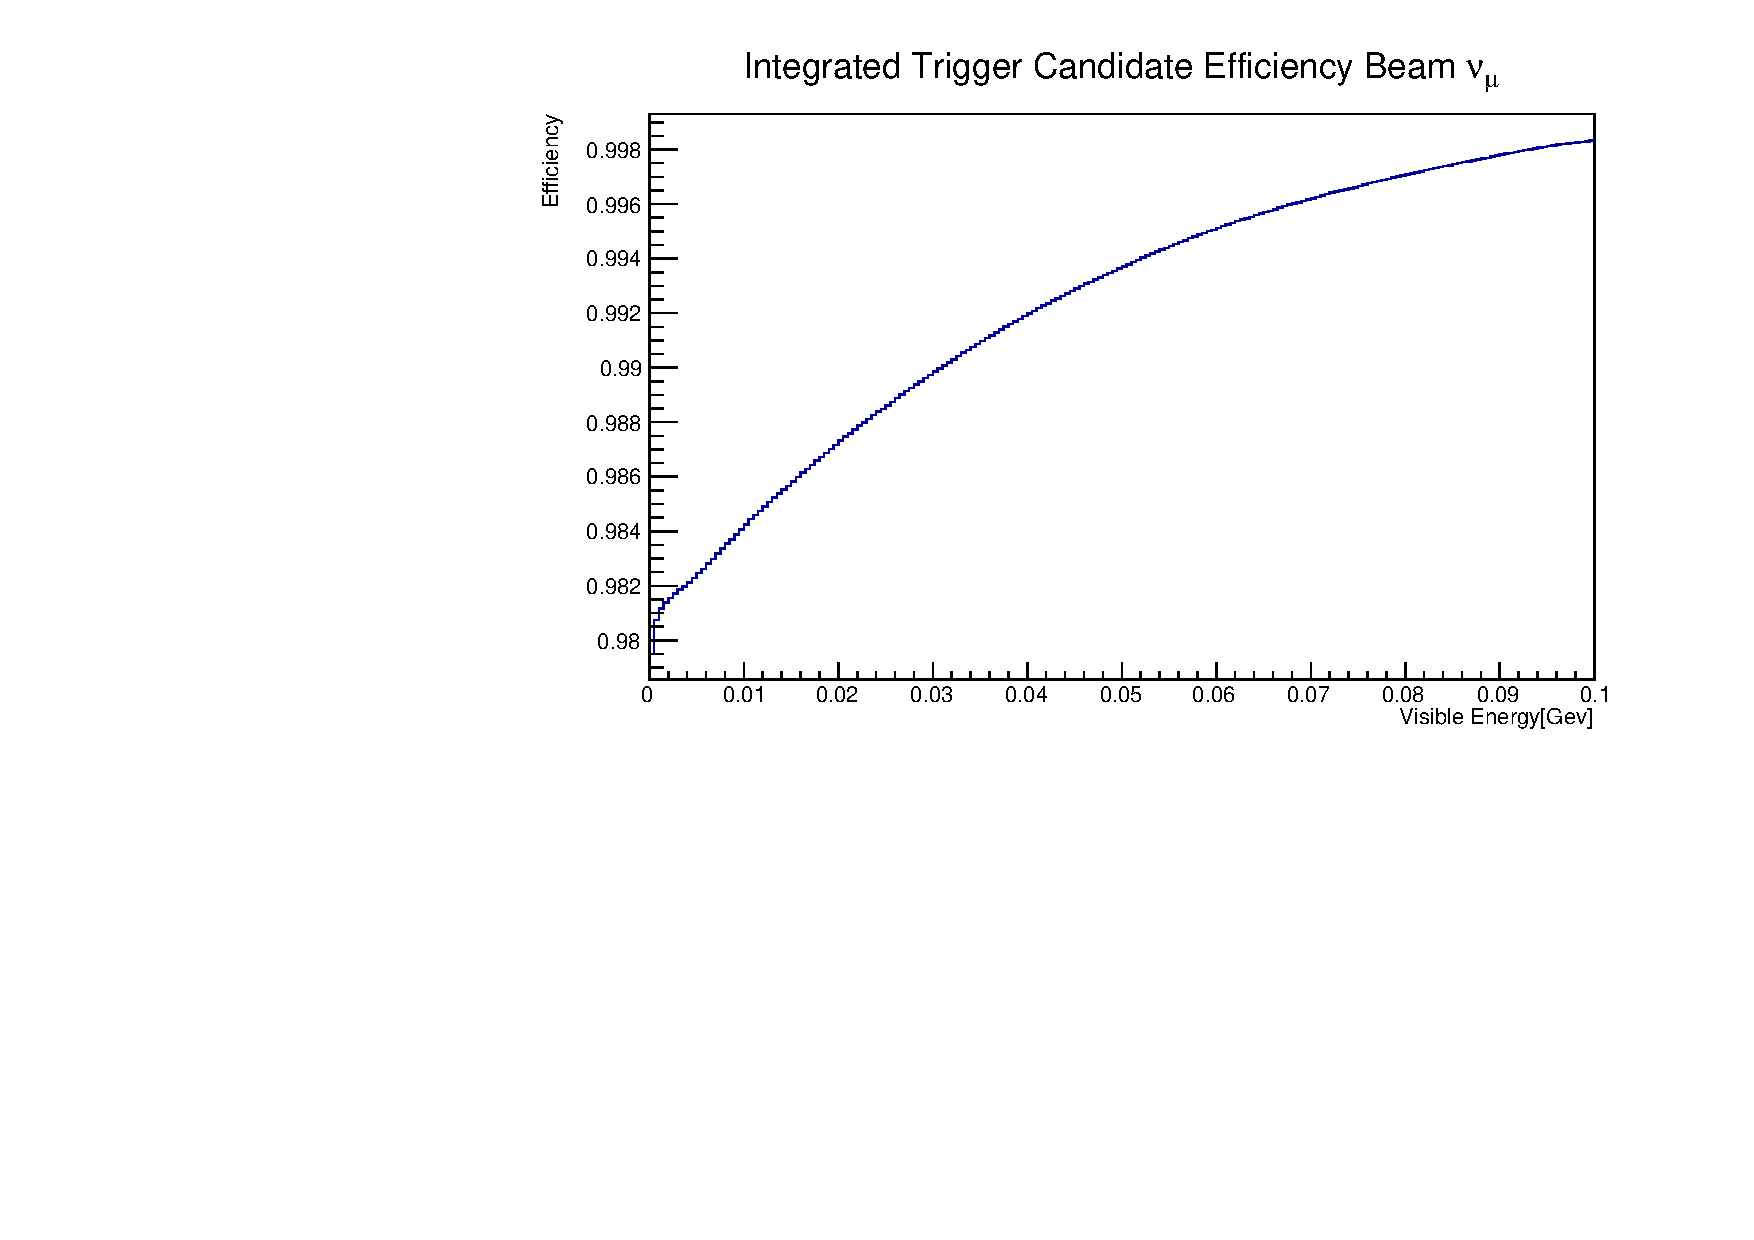
\includegraphics[width=0.45\textwidth]{Integrated_Nu_mu_Efficiency_MCC10.pdf}
\end{dunefigure}


Trigger candidate generation, building on trigger primitives and defined
as two consecutive trigger primitives in both channel and time space,
with a minimum hit threshold, have also been studied with MonteCarlo
simulations.
Trigger candidates with sufficient energy can be accepted to generate
corresponding Trigger Commands for localized high energy activity, such
as for beam, atmospheric neutrinos, baryon number violating signatures,
and cosmics.
Simulation studies demonstrate that this scheme meets efficiency
requirements for localized high energy triggers, as shown in
Figure~\ref{fig:daq-tc-eff-vis}.
Specifically, simulations demonstrate that $>99$\% \hlfix{efficiency is
  achievable}{This is for SP, needs redo with DP} for $>100$ MeV visible
energy, and that the effective threshold for localized triggers for the
system is at $\sim$10 MeV. 

Low-energy trigger candidates furthermore can serve as input to the SNB
trigger.
Simulation demonstrates that the trigger candidate efficiency for any
individual SN neutrino interaction is on the \hlfix{order of 20-30\%}{SP
  number}.
Simulations have further demonstrated that a multiplicity-based SNB
trigger decision which integrates low-energy trigger candidates over an
up to 10 seconds integration window yields high ($>90$\%) galactic
coverage while keeping fake SNB trigger rates to one per month, per
system requirements.
An energy-weighted multiplicity count scheme could be applied to further
increase efficiency and minimize background.
The dominant contributor to fake SNB triggers is radiological
backgrounds from neutrons, followed by Radon. It is crucial to continue
working closely with the Radiological Task force to validate
radiological simulation assumptions.

Given that simulation studies support requirements and rate assumptions,
the protoDUNE demonstration of ability to keep up with rates from
1/25$^{th}$ the size of a single DUNE FD SP module, for trigger rates up
to 40 Hz and 3 ms readout window allows confident scaling of the
protoDUNE back-end DAQ subsystem to that of DUNE.

The developments described above can be also naturally deploied at the level of ProtoDUNE dual-phase. In a second run of
protoDUNE dual-phase it will be possible to replace the Mellanox 10 Gbit ethernet cards in the level 1 event builders with Felix cards in order to fully
test the DUNE data acquisition mode and the on the fly decompression and generation of trigger primitives. The Felix cards can also operate as standard
network cards and should offer completely backward compatibility with the standard operation mode of protoDUNE-DP which is based on external triggers.
and the switch for dedicated tests, switch to the DUNE mode with  continuos data streaming,  on the fly data decompression + trigger primitives generation in the Felix card,  RAM buffering of the compressed data on the LV1 event builders, writing of the data on disk after receiving the trigger from the trigger filtering machine. A trigger filtering machine can be integrated in the 40 Gbit/s network architecture of protoDUNE dual-phase in order to control the persistent data writing. The EOS online storage system of protoDUNE dual-phase provides a bandwidth of 20GB/s and it would be sufficient to ensure the data storage for a 10 kton dual-phase module. This architecture offers also the possibility to test the SNa data buffering (for 10 seconds) and data writing in dedicated tests. This test phase where the entire protoDUNE dual-phase is switched to the DUNE online trigger mode can be anticipated by simpler tests at the level of a single crate where the development chain already operating in Lyon and described in Section~\ref{sec:daq:validation-demonstrators} could be transported to protoDUNE dual-phase for the readout of a single crate.


\subsubsection{Prototype Inter-process Communication System}

A prototype of the \dword{ipc} mechanism described in
Section~\ref{sec:daq:design-ipc} is currently under development and testing at
\dword{protodune}. 
Goals of this prototype include evaluating throughput and rate limitations,
understanding message schema and application level protocols, prototyping CCM
functionality including \dword{daqdispre}, investigating scaling and software
complexity management as well as providing functional support for other tests of
the DUNE FD DAQ design at \dword{protodune}.

Initial offline prototype tests have demonstrated ZeroMQ inter-thread transport
is more than sufficient for use in the highest rate \dword{daq} context (input
to \dword{trigprimitive} production).
Tests with small packets have demonstrated ZeroMQ's ability to handle the high
packet rate of \dword{trigprimitive} or trigger candidate data over all three of
the ZeroMQ transport mechanisms that are being considered for use (inter-thread,
inter-process and network).  

ZeroMQ IPC has been successfully exercised at \dword{protodune} as part of a
practical solution to transfer the full stream of trigger primitives out of one
process and in to another. 
This tests the eventual leg between producers of trigger primitives and their
consumers (trigger candidate processors). 
The merging of multiple, asynchronous trigger primitive streams into a single
ordered stream which is properly prepared for input to trigger candidate
processing has been developed and tested offline. 
Performance testing and integration into the self-triggering prototype at
\dword{protodune} is in progress.


\subsection{Additional Teststands}
\label{sec:daq:validation-demonstrators}

Concurrently with protodune operation and development, a number of
``vertical slice'' teststands will be built to allow 
development and testing of individual parts of the \dword{daq} system
as well as testing of key aspects of the design and overall
scalability. A data selection subsystem vertical slice teststand will be
constructed and operated on fake-generated data, to assist in the
development of data selection, exercise the system for a variety of
configurations, perform small-scale tests that stress the critical
parts of the corresponding infrastructure, 
and identify likely failure points and/or bottlenecks. The subsystem
will also be deployed and exercised on existing HPC clusters of
comparable resources and specifications as planned for the final
production system for ``horizontal slice'' tests of similar nature. The
back-end DAQ subsystem will be developed and tested in a similar way.

In addition to dedicated vertical and horizontal slice teststands, a number of
\dword{daq} ``development kits'' will be available for the consortium for
specific component testing, as well as to other detector and
calibration consortia to support their own development, production, and quality assurance programs. The \dword{daq} 
kit will also form the basis for testing at construction sites beginning in 2020. 

A complete demonstration system in order to test the DUNE dual-phase DAQ has been put in operation at IPNL. This system
includes a charge readout uTCA crate with 10 AMC cards and a DAQ server including a FPGA network card (Bittware A10P3S with Altera Arria 10 FPGA,
4 x 40 GbE QSFP interfaces which can support  x16 10 GbE channels). The purpose of this system is to test the firmware developments in the AMCs for the DUNE continous streaming DAQ operation and  to develop the backend firmware for data reception, decoding, decompression and generation of trigger primitives. The data reception and real time decompression have already been implemented with a high degree of parallelism in the Arria 10 FPGA and are already operational. The implementation of the generation of the trigger primitives at the FPGA level after decompression is in progress. The digital front-end electronics at the level of the AMCs can operate in both trigger based mode (ProtoDUNE-DP) or continous streaming mode (DUNE). This test chains allows performing all the demonstration and benchmarking steps without interferring with the ProtoDUNE-DP DAQ operation which is trigger based. This benchmarking phase is in particular useful in order to correctly dimension the DUNE DAQ for the dual-phase far detector module. The algorithms and the firmware developed on the Arria 10 FPGA could be then trasnported at the level of the Felix card or other DAQ elements of the DUNE DAQ. The Bittware A10P3S could also be at a certain point plugged in protoDUNE DP replacing one of the Mellanox ethernet cards of the level 1 event builders in order to provide a direct demonstration with real data.


\section{Production, Assembly, Installation and Integration}
\label{sec:daq:production}

\fixme{This will be completed at a later time.}

\subsection{Production and Assembly}
\metainfo{Describe how hardware, firmware and software will produced. }

\subsubsection{Computing Hardware}

\subsubsection{Custom Hardware Fabrication}

\subsubsection{Software and Firmware Development}
\metainfo{Processes and practices.}

\subsection{Installation and Integration}

\section{Organization and Project Management}
\label{sec:daq:organization}

\subsection{Consortium Organization}

The DAQ Consortium was formed in 2017 as a joint single and dual phase
consortium, with a Consortium Leader and a Technical Leader.
The organization of the consortium is shown in Figure~\ref{fig:daq-org}.
The DAQ consortium board currently comprises institutional representatives from
30 institutes as shown in Table~\ref{tab:daq-ib}.
The consortium leader is the spokesperson for the consortium and responsible for
the overall scientific program and management of the group.
The technical leader of the consortium is responsible for managing the project
for the group.

The consortium's initial mandate has been the design, construction, and
commissioning of the DUNE FD DAQ system.
To realize this, the consortium was initially organized in the form of five
working groups: (1) Architecture, (2) Hardware, (3) Data Selection, (4) Back-end
DAQ, and (5) Installation and Infrastructure.
This organization has seen the project through the conceptual design phase.  

A new organizational structure has been adopted to see the project through
engineering design and construction, and this structure is expected to evolve in
order to meet the needs of the consortium.
This is shown in Figure~\ref{fig:daq-org}.
Each working group has a designated working group leader.
In addition to the working group leads, technical design report editors are
responsible for the overall editing and delivery of the TDR document.

\fixme{This is DRAFT/IN DEVELOPMENT. From Giovanna; needs consortium input. }
\begin{dunefigure}{fig:daq-org}{Organizational chart for the \dword{daq} Consortium
 }
  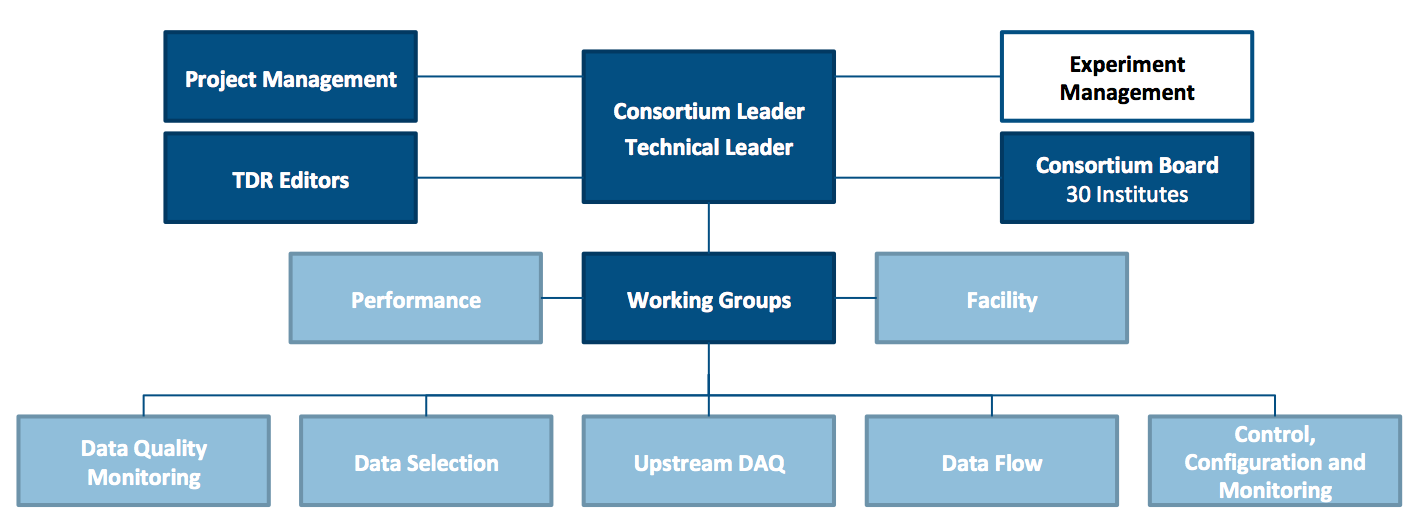
\includegraphics[width=0.8\textwidth]{daq-org.png}
\end{dunefigure}

\fixme{This is DRAFT. Needs consortium vetting. }
\begin{dunetable}
[DAQ Consortium Board institutional members and countries]
{p{0.65\textwidth}p{0.25\textwidth}}
{tab:daq-ib}
{DAQ Consortium Board institutional members and countries.}   
Member Institute & County  \\ \toprowrule
CERN & CERN     \\ \colhline
Universidad Sergio Arboleda (USA) & Colombia     \\ \colhline
APC Paris & France \\ \colhline
IPNL Lyon & France \\ \colhline
Iwate & Japan     \\ \colhline
KEK & Japan     \\ \colhline
NIT Kure & Japan     \\ \colhline
NIKHEF & Netherlands    \\ \colhline
University of Birmingham & UK     \\ \colhline
Bristol University & UK     \\ \colhline
University of Edinburgh & UK     \\ \colhline
Imperial College London & UK     \\ \colhline
University of Liverpool & UK     \\ \colhline
Oxford University & UK     \\ \colhline
Rutherford Appleton Lab (RAL) & UK     \\ \colhline
University of Sussex Sussex & UK     \\ \colhline
University College London (UCL) & UK     \\ \colhline
University of Warwick & UK     \\ \colhline
Brookhaven National Lab (BNL) & USA     \\ \colhline
Colorado State University (CSU) & USA     \\ \colhline
Columbia University  & USA     \\ \colhline
University of California, Davis (UCD) & USA     \\ \colhline
Duke University & USA     \\ \colhline
University of California, Irvine (UCI) & USA     \\ \colhline
Fermi National Lab (FNAL) & USA     \\ \colhline
Iowa State University & USA     \\ \colhline
University of Minnesota, Duluth (UMD) & USA     \\ \colhline
University of Notre Dame & USA     \\ \colhline
University of Pennsylvania (Penn) & USA     \\ \colhline
Pacific Northwest National Lab (PNNL) & USA     \\ \colhline
South Dakota School of Mines and Technology (SDSMT) & USA     \\ \colhline
Stanford Linear Accelerator Lab (SLAC) & USA     \\ \colhline
\end{dunetable}

\subsection{Cost and Labor}
\label{sec:daq:cost}

\fixme{Table~\ref{tab:Xsched} is a standard table template for the TDR
  schedules. 
  It contains overall FD dates from Eric James as of March 2019 (orange) that
  are held in macros in the common/defs.tex file so that the TDR team can change
  them if needed. Please do not edit these lines! Please add your milestone
  dates to fit in with the overall FD schedule. Please set captions and label
  appropriately. Anne}


Table~\ref{tab:daq-cost} shows the current cost estimates for the DAQ subsystems
major components necessary to serve the first DUNE FD module.
Costs are expected to be reduced for subsequent modules, since multiple
components are common across modules.
When appropriate, the quantities of components are shown, along with the total
cost and a brief description of what is included in the cost estimate.
The cost estimates include materials and supplies (M\&S) for construction, and
packing and shipping to SURF, but not labor and travel costs for construction,
or spares. 

Labor costs depend on personnel category (e.g., faculty, student,
technician, post-doc, engineer), and vary by region and
institution. As such, costs are quantified using labor hours needed to
fulfil a given task. Table~\ref{tab:daq-labor} provides estimates of
labor hours for each subsystem. Signficant physics and simulation
effort is needed in particular for data selection related studies; those
labor resources are listed separately.

\begin{dunetable}
[DAQ System Cost Summary]
{p{0.15\textwidth}p{0.1\textwidth}p{0.15\textwidth}p{0.4\textwidth}}
{tab:daq-cost}
{Cost estimates for different DAQ subsystems. All cost estimates
  include M\&S for construction only. Packing and shipping costs are
  included; spares are not included. \fixme{These are SP numbers.}}   
System & Quantity & Cost (under development) (k\$ US) & Description \\ \toprowrule
TPC Front-end Readout & 75 & - & Felix and co-processor, host server, and networking  \\ \colhline
PDS Front-end Readout & 6-8 & - & Felix, host server, and networking  \\ \colhline
Low-Level TPC Data Selection & 75 & -&  \\ \colhline
Low-Level PDS Data Selection & 6-8 & -&  \\ \colhline
High-Level PDS Data Selection & 1 & - & MLT, EXT and interface boards, High-Level Filter
Networking \\ \colhline
Back-end DAQ & & - & \\ \colhline 
\end{dunetable}

\begin{dunetable}
[DAQ System Labor]
{p{0.25\textwidth}p{0.15\textwidth}p{0.1\textwidth}p{0.08\textwidth}p{0.08\textwidth}p{0.1\textwidth}p{0.08\textwidth}}
{tab:daq-labor}
{Estimate of labor hours for each category of personnel for different DAQ subsystems.}
System  & Faculty/Scientist & Post-doc & Student & Engineer & Technician  &  \textbf{Total}\\ \toprowrule
& (hours) & (hours)& (hours)& (hours)& (hours)& (hours)\\ \toprowrule
Upstream DAQ & -& -& -& -& - & - \\ \colhline
Data Selection & -& -& -& -& - & - \\ \colhline
Back-end DAQ & -& -& -& -& - & - \\ \colhline
Software Infrastructure & -& -& -& -& - & - \\ \colhline
CCM & -& -& -& -& - & - \\ 
Physics \& Simulation & -& -& -& -& - & - \\ \colhline
\end{dunetable}

Following the funding model envisioned for the consortium, various
responsibilities have been distributed across institutions within the
consortium. At this stage of the project, these should be considered
as ``aspirational'' responsibilities until firm funding decisions are
made. Table~\ref{tab:daq-inst-resp} shows the current institutional
responsibilities for primary DAQ subsystems. Only lead institutes are
listed in the table for a given effort. For physics and simulation
studies, and validation efforts at ProtoDUNE, wider institutional effort is
involved. A detailed list of tasks and institutional responsibilities
are presented in \cite{WBS}.

\begin{dunetable}
[DAQ System Institutional Responsibilities]
{p{0.65\textwidth}p{0.25\textwidth}}
{tab:daq-inst-resp}
{Institutional responsibilities in the DAQ Consortium}
DAQ Sub-system  & Institutional Responsibility\\ \toprowrule
Front-end Readout & Institutes \\ \colhline
Data Selection & Institutes \\ \colhline
Back-end DAQ & Institutes\\ \colhline
IPC & Institutes \\ \colhline
CCM & Institutes \\ 
Physics \& Simulation & Institutes\\ \colhline
\end{dunetable}

\subsection{Schedule and Milestones}
\label{sec:daq:schedule}

\begin{dunetable}
[DAQ Consortium Schedule]
{p{0.65\textwidth}p{0.25\textwidth}}
{tab:DAQ-sched}
{DAQ Consortium Schedule}   
Milestone & Date (Month YYYY)   \\ \toprowrule
Technology Decision Dates &      \\ \colhline
Final Design Review Dates &      \\ \colhline
Start of module 0 component production for ProtoDUNE-II &      \\ \colhline
End of module 0 component production for ProtoDUNE-II &      \\ \colhline
\rowcolor{dunepeach} Start of \dword{pdsp}-II installation& \startpduneiispinstall      \\ \colhline
\rowcolor{dunepeach} Start of \dword{pddp}-II installation& \startpduneiidpinstall      \\ \colhline
 \dword{prr} dates &      \\ \colhline
Start of  (component 1) production  &      \\ \colhline
Start of (component 2) production  &      \\ \colhline
Start of  (component 3) production  &      \\ \colhline
\rowcolor{dunepeach}South Dakota Logistics Warehouse available& \sdlwavailable      \\ \colhline
\rowcolor{dunepeach}Beneficial occupancy of cavern 1 and \dword{cuc}& \cucbenocc      \\ \colhline
\rowcolor{dunepeach} \dword{cuc} counting room accessible& \accesscuccountrm      \\ \colhline
\rowcolor{dunepeach}Top of \dword{detmodule} \#1 cryostat accessible& \accesstopfirstcryo      \\ \colhline
End of  (component 1) production  &      \\ \colhline
... & ...                       \\ \colhline
\rowcolor{dunepeach}Start of \dword{detmodule} \#1 TPC installation& \startfirsttpcinstall      \\ \colhline
\rowcolor{dunepeach}End of \dword{detmodule} \#1 TPC installation& \firsttpcinstallend      \\ \colhline
\rowcolor{dunepeach}Top of \dword{detmodule} \#2 accessible& \accesstopsecondcryo      \\ \colhline
 \rowcolor{dunepeach}Start of \dword{detmodule} \#2 TPC installation& \startsecondtpcinstall      \\ \colhline
\rowcolor{dunepeach}End of \dword{detmodule} \#2 TPC installation& \secondtpcinstallend      \\ \colhline
last item & ...                         \\
\end{dunetable}

\subsection{Safety and Risks}

